\documentclass[10pt]{article}
%%%%%%%%%%%%%%%%%%%%%%%%%%%%%%%%%%%%%%%%%%
%	Included Packages
%%%%%%%%%%%%%%%%%%%%%%%%%%%%%%%%%%%%%%%%%%
\usepackage{times}
\usepackage{amsmath}
\usepackage{enumerate}

\usepackage{hyperref}
\usepackage[labelfont=bf]{subcaption}
\usepackage{graphicx,latexsym,float}
\usepackage{fancyhdr}
\usepackage{alltt}
\usepackage{listings}
\usepackage{epstopdf}
\usepackage{color}
\usepackage[labelfont=bf]{caption}
\usepackage{tabu}
\usepackage{xspace}
\usepackage{multicol}

%%%%%%%%%%%%%%%%%%%%%%%%%%%%%%%%%%%%%%%%%%
%	Document Formatting
%%%%%%%%%%%%%%%%%%%%%%%%%%%%%%%%%%%%%%%%%%
\tabulinesep=1.2mm 
\setlength{\textheight}{9.0in}
\setlength{\oddsidemargin}{0in}
\setlength{\evensidemargin}{0in}
\setlength{\topmargin}{-0.25in}
\setlength{\textwidth}{6.5in}

%\setlength{\textfloatsep}{0.1cm}
% add space between paragraphs
%\setlength{\parskip}{0.5em}

\pagestyle{fancy}
\fancyhead[L]{}
\fancyhead[R]{}
\fancyhead[C]{}
\fancyfoot[L]{}
\fancyfoot[R]{}
\fancyfoot[C]{}

\fancyhead[L]{\slshape \rightmark}
\fancyhead[R]{\thepage}

%%%%%%%%%%%%%%%%%%%%%%%%%%%%%%%%%%%%%%%%%%
%	Image Path
%%%%%%%%%%%%%%%%%%%%%%%%%%%%%%%%%%%%%%%%%%
\graphicspath{{./TechReportAndDocumentation_files/}}

%%%%%%%%%%%%%%%%%%%%%%%%%%%%%%%%%%%%%%%%%%%%%%%
%	New command definitions/redefinitions
%%%%%%%%%%%%%%%%%%%%%%%%%%%%%%%%%%%%%%%%%%%%%%%

% remake the texttt command so that line breaks will occur for certain
% characters
\renewcommand{\texttt}[1]{%
  \begingroup
  \ttfamily
  \begingroup\lccode`~=`/\lowercase{\endgroup\def~}{/\discretionary{}{}{}}%
  \begingroup\lccode`~=`[\lowercase{\endgroup\def~}{[\discretionary{}{}{}}%
  \begingroup\lccode`~=`.\lowercase{\endgroup\def~}{.\discretionary{}{}{}}%
  %\begingroup\lccode`~=`:\lowercase{\endgroup\def~}{:\discretionary{}{}{}}%
  \catcode`/=\active\catcode`[=\active\catcode`.=\active
  \scantokens{#1\noexpand}%
  \endgroup
}

% Colors used for Java code
\definecolor{dkgreen}{rgb}{0,0.6,0}
\definecolor{gray}{rgb}{0.5,0.5,0.5}
\definecolor{mauve}{rgb}{0.58,0,0.82}

\lstset{frame=tb,
  language=Java,
  aboveskip=3mm,
  belowskip=3mm,
  showstringspaces=false,
  columns=flexible,
  basicstyle={\small\ttfamily},
  numbers=left,
  numberstyle=\tiny\color{gray},
  keywordstyle=\color{blue},
  commentstyle=\color{dkgreen},
  stringstyle=\color{mauve},
  breaklines=true,
  breakatwhitespace=true,
  tabsize=3,
  escapeinside={||}
}

\newcommand{\env}[1]{{\texttt{#1}}}
\newcommand{\fil}[1]{{\em #1}}
\newcommand{\cls}[1]{{\texttt{#1}}}
\newcommand{\sig}[1]{{\em #1}}
\newcommand{\pkg}[1]{{\texttt{#1}}}
\newcommand{\opt}[1]{{\em #1}}
\newcommand{\pgm}[1]{{\textbf{#1}}}
\newcommand{\dir}[1]{{\em #1}}
\newcommand{\sbr}[1]{{\em #1}}
\newcommand{\MYhref}[3][blue]{\href{#2}{\color{#1}{#3}}}%

\newcommand{\state}[1]{{\bf #1}}
\newcommand{\AND}{\bullet}
\newcommand{\nnp}{\newpage}
\newcommand{\nni}{\noindent}
\newcommand{\nnpi}{\newpage \noindent}
\newcommand{\textQuote}[1]{\textquotedblright{#1}\textquotedblright}
\newcommand{\bel}{\cls{Bel}\xspace}
\newcommand{\bels}{\cls{Bel}s\xspace}
\newcommand{\site}{\cls{Site}\xspace}
\newcommand{\sites}{\cls{Site}s\xspace}
\newcommand{\cell}{\cls{Cell}\xspace}
\newcommand{\cells}{\cls{Cell}s\xspace}
\newcommand{\cellpin}{\cls{CellPin}\xspace}
\newcommand{\cellpins}{\cls{CellPin}s\xspace}
\newcommand{\belpin}{\cls{BelPin}\xspace}
\newcommand{\belpins}{\cls{BelPin}s\xspace}
\newcommand{\tile}{\cls{Tile}\xspace}
\newcommand{\tiles}{\cls{Tile}s\xspace}
\newcommand{\cellnet}{\cls{CellNet}\xspace}
\newcommand{\cellnets}{\cls{CellNet}s\xspace}
\newcommand{\net}{\cls{Net}\xspace}
\newcommand{\nets}{\cls{Net}s\xspace}
\newcommand{\port}{\cls{Port}\xspace}
\newcommand{\ports}{\cls{Port}s\xspace}
\newcommand{\celldesign}{\cls{CellDesign}\xspace}
\newcommand{\sitepin}{\cls{SitePin}\xspace}
\newcommand{\sitepins}{\cls{SitePin}s\xspace}
\newcommand{\routeTree}{\cls{RouteTree}\xspace}
\newcommand{\routeTrees}{\cls{RouteTree}s\xspace}
\newcommand{\pip}{\cls{PIP}\xspace}
\newcommand{\pips}{\cls{PIP}s\xspace}

\newenvironment{codei}{\vspace{-0.1in} \begin{center} \begin{minipage}{6in} \noindent \begin{alltt}}{\end{alltt} \end{minipage} \end{center}}
\newenvironment{code}{\begin{center} \begin{minipage}{6in} \noindent \begin{alltt}}{\end{alltt} \end{minipage} \end{center}}

\makeatletter

\newcommand\problem{\@startsection{problem}{3}{\z@}%
                                     {-3.25ex\@plus -1ex \@minus -.2ex}%
                                     {1.5ex \@plus .2ex}%
                                     {\normalfont\normalsize\bfseries}}
\makeatother

\makeindex
% show all sections (even subsections and subsubsections in the table of contents)
\setcounter{tocdepth}{3}

%%%%%%%%%%%%%%%%%%%%%%%%%%%%%%%%%%%%%%%%%%
%	Document Start
%%%%%%%%%%%%%%%%%%%%%%%%%%%%%%%%%%%%%%%%%%
\begin{document}

%%%%%%%%%%%%%%%%%%%%%%%%%%%%%%%%%%%%%%%%%%
%	Formatting
%%%%%%%%%%%%%%%%%%%%%%%%%%%%%%%%%%%%%%%%%%
\floatstyle{ruled}
\newfloat{Program}{thp}{loa}[section]

\date{}

%%%%%%%%%%%%%%%%%%%%%%%%%%%%%%%%%%%%%%%%%%
%	Title
%%%%%%%%%%%%%%%%%%%%%%%%%%%%%%%%%%%%%%%%%%
\title{{\bf \Huge \sc{RAPIDSMITH2}}\\[0.1in]
A Library for Low-level Manipulation 
of Vivado Designs at the Cell/BEL Level\\[0.3in]
Technical Report and Documentation\\[0.1in]
}
\author{\Large Brent Nelson, Thomas Townsend, and Travis Haroldsen\\[0.2in]
\large NSF Center for High Performance Reconfigurable Computing (CHREC) \thanks{This work was supported in part by the I/UCRC program of the National
 Science Foundation, grant numbers 0801876 and 1265957.}\\
\large Department of Electrical and Computer Engineering  \\
\large  Brigham Young University \\
\large  Provo, UT, 84602 \\[0.7in]
\large Last Modified: \today \\[0.05in]
}


\maketitle
\begin{figure}[H]
\centering
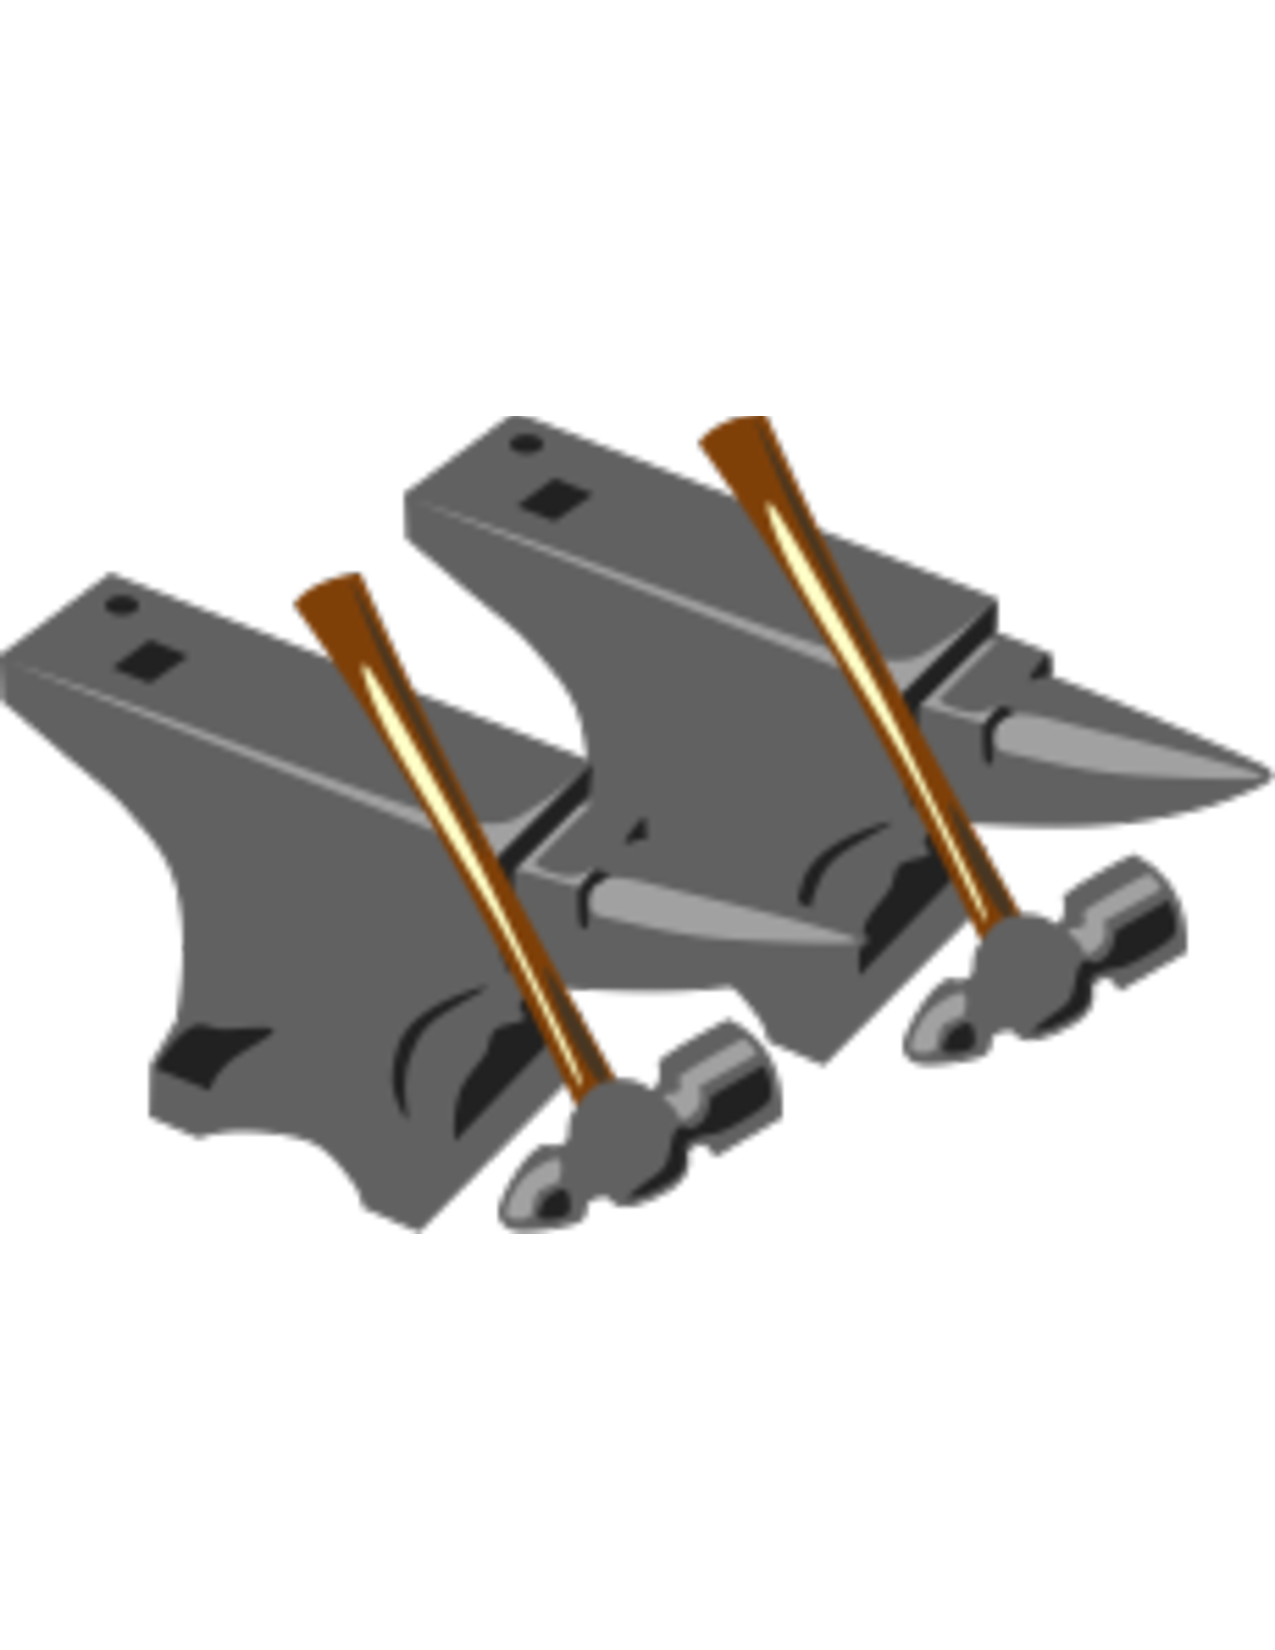
\includegraphics[width=0.4\columnwidth]{logo}
\end{figure}

%%%%%%%%%%%%%%%%%%%%%%%%%%%%%%%%%%%%%%%%%%
%	Table of Contents
%%%%%%%%%%%%%%%%%%%%%%%%%%%%%%%%%%%%%%%%%%
\newpage
\tableofcontents

%%%%%%%%%%%%%%%%%%%%%%%%%%%%%%%%%%%%%%%%%%
%	Tech Report Chapters
%%%%%%%%%%%%%%%%%%%%%%%%%%%%%%%%%%%%%%%%%%
%%%%%%%%%%%%%%%%%%%%%%%%%%%%%%%%%%%%%%%%%%%%%%%%%%%%%%%%%%%%%%%%
% Section 1: Introduction
%%%%%%%%%%%%%%%%%%%%%%%%%%%%%%%%%%%%%%%%%%%%%%%%%%%%%%%%%%%%%%%%
\newpage
\section{Introduction}
\subsection{What is RapidSmith2?}
The original BYU RapidSmith project began in 2010. Its goal was to develop
a set of tools and APIs which would provide academics with an
easy-to-use platform to implement experimental CAD ideas and algorithms on
modern Xilinx FPGAs. It integrated with Xilinx's old design suite, ISE.
RapidSmith2 represents a major addition to RapidSmith. Specifically, Vivado
designs are now supported. Using RapidSmith2 you can write custom CAD tools
which will:

\begin{itemize}
  \item Export designs from Vivado
  \item Perform analyses on those designs
  \item Make modifications to those designs
  \item Import those designs back into Vivado for further processing or
  bitstream generation
\end{itemize}
Futhermore, you need not start with a Vivado design --- 
you can create a new design from scratch in RapidSmith2 and then import it into Vivado
if desired.

The other new major capability of RapidSmith2 is that it changes RapidSmith's design
representation. Instead of using XDL's view of a design with Instances and
Sites, RapidSmith2 uses Vivado's representation of design with Cells and BELs. This
is a significant change as it exposes the actual design and device in a way
that RapidSmith never did, opening up new CAD research opportunities which were
difficult to perform using Rapidsmith.
       
\subsection{Who Should Use RapidSmith2?}
RapidSmith2 is aimed at anyone desiring to do FPGA CAD research on real Xilinx devices
available in Vivado. As such, users of RapidSmith2 should have some understanding of
Xilinx FPGA architecture, the Vivado design suite, and the Tcl programming
language. However, one goal of this documentation is to provide sufficient
background and detail to help bring developers up to speed on the needed
topics. RapidSmith2 is by no means a Xilinx Vivado replacement. It cannot be used
without a valid and current license to a Vivado installation (RapidSmith2
cannot generate bitstreams for example).

\subsection{Why RapidSmith2?}
The Xilinx-provided Tcl interface into Vivado is a great addition to the tool
suite. It can be used to do a variety of useful things including scripting
design flows, querying device and design data structures, and  modifying placed
and routed designs. In theory, the Tcl interface provides all of the
functionality needed in order to create any type of CAD tool as a plugin to the
normal Vivado tool flow. However, there are a few issues in TCL that motivate
the use of external CAD tool frameworks such as RapidSmith2. These include:
\begin{itemize}
  \item Tcl, being an interpreted language, is slow. It is far too slow to
  implement complex algorithms such as PathFinder. Compiled and
  managed runtime languages are a better option in terms of performance.
  \item Tcl is hard to program in. TCL is not an object oriented language, and
  so writing complex algorithms are difficult since Object-Oriented language
  constructs do not exist. That being said, TCL is great for writing automation
  scripts.
  \item There are some memory issues in Vivado's Tcl interface. In our
  experience, long-running scripts eventually cause the system to run out of
  memory even if they are not doing anything interesting.
  \item Vivado's TCL interface does not offer a complete device representation
  (determined by Brad White's MS work). Most notably, a user cannot gain
  access to sub-site wire objects through the Tcl interface. This limits the CAD
  tools that can be created in Tcl, but this additional information can be added
  to external tools with some manual work.
\end{itemize}

\noindent
In short, the ability to export designs out of Vivado, manipulate them with more
powerful languages such as Java, and then import the design back into Vivado
is a very useful capability.

RapidSmith2 (in conjunction with Tincr - see Section~\ref{sec:tincr}) abstracts
this process into a few easy-to-use function calls. Generating FPGA part information, importing and exporting \pgm{all aspects} of a design, and dealing with other fairly arcane details is made mostly transparent to the
user. RapidSmith2 and Tincr provide a nice API into equivalent Vivado device and design
data structures. All of this enables researchers to have more time to focus on what matters
most: the research of new ideas and algorithms.

\subsection{How is RapidSmith2 Different than VPR and VTR?}
VPR (Versatile Place and Route) has been an FPGA research tool for several years
and has led to many publications on new FPGA CAD research. It has been a
significant contribution to the FPGA research community and has grown to be a
complete FPGA CAD flow for research-based FPGAs. The main difference between
RapidSmith/RapidSmith2 and VPR is that the RapidSmith tools can target commercial Xilinx
FPGAs, providing the ability to exit and re-enter the standard Xilinx flow at
any point.  All features of commercial FPGAs which are accessible via XDL and
Vivado's Tcl interface are available in RapidSmith and RapidSmith2. VPR is currently
limited to FPGA features which can be described using VPR's architectural
description facilities.

\subsection{Why Java?}
RapidSmith2 is written in Java. We have found Java to be an excellent rapid prototyping
platform for FPGA CAD tools.  Java libraries are rich with useful data
structures, and garbage collection eliminates the need to clean up objects in
memory. This helps reduce the time spent debugging, leaving more
time for researchers to focus on the real research at hand.  Our experience over
the past decade is that for student research projects, Java has greatly improved
student productivity and led to far more stable CAD tools.

\subsection{Using This TechReport and Getting Started}
This technical report was written to serve two purposes.  The first is to
provide information for new users to get started using RapidSmith2.  The second
is that it also contains detailed reference information for both more advanced
users as well as for those who maintain RapidSmith2.  

If you are a new user we suggest you use this document in the following ways:

\begin{enumerate}
  \item Start by reading Sections 1-3 carefully.
  \item Experiment with the use of the example programs discussed in
  Section~\ref{examples}.  Then use those along with the example designs
  provided in the \dir{exampleVivadoDesigns} directory of the RapidSmith2
  repository.  Finally, move on to using your own designs.
  In particular, focus on learning to export/import designs to/from Vivado and
  how to use some the basic functions like the pretty printer and DOT file
  generator.
  \item Then, work your way through the tutorials in the file
  \dir{docs/Exercises/Exercises.pdf}.
  \item Finally, begin working on your own projects.
\end{enumerate}

As you read through this technical report initially, note the advanced topics
sections and skim or skip them entirely.  As you become more experienced and/or
have a need, those advanced sections will provide important reference material
for you to learn many of the important details associated with RapidSmith2.  As you
become more experienced, don't neglect to generate and read the JavaDoc
documentation for the actual source code.  Finally, the source code itself can
be an important way of understanding parts of  RapidSmith2's features and
functionality.

%%%%%%%%%%%%%%%%%%%%%%%%%%%%%%%%%%%%%%%%%%%%%%%%%%%%%%%%%%%%%%%%%%%%%%%%%%%%
% Section 2: Background Information of RapidSmith, RapidSmith2, and Tincr
%%%%%%%%%%%%%%%%%%%%%%%%%%%%%%%%%%%%%%%%%%%%%%%%%%%%%%%%%%%%%%%%%%%%%%%%%%%%
\newpage
\section{Background}

\graphicspath{{./techReportFigures/sec2_background/}}

RapidSmith2 is based on the original RapidSmith project written by Christopher
Lavin as a part of his PhD work at BYU.  It was based on the Xilinx Design
Language (XDL) which provides a human-readable file format equivalent to the
Xilinx proprietary Netlist Circuit Description (NCD) of \textbf{ISE}.  With
RapidSmith, researchers were able to import XDL, manipulate, place, route and export
designs among a variety of design transformations.  The RapidSmith project made
an excellent test bed to try out new ideas and algorithms for FPGA CAD research
because code could quickly be written to take advantage of the APIs available.
RapidSmith also contained packages which could parse/export bitstreams (at the
packet level) and represent the frames and configuration blocks in the provided
data structures. RapidSmith continues to be functional and is still available at
{\color{blue} http://rapidsmith.sourceforge.net/}. There, you will find
documentation, installation instructions, the RapidSmith code base, and a
collection of demo programs demonstrating example CAD tools.

RapidSmith is a great contribution to the FPGA community, but as previously
stated is built upon the XDL interface offered in Xilinx's ISE tools suite.
Unfortunately, Vivado (Xilinx's newest tool suite) does not support XDL. This
makes CAD tools based on XDL incompatible with next-generation Xilinx devices
such as UltraScale and UltraScale+. Instead, Vivado offers a Tcl interface
that can potentially be used to extract Xilinx device and design information.
The ultimate goal of RapidSmith2 is to update the original RapidSmith to support
implementing CAD tools with Vivado designs. The remainder of this section gives
an overview of the required components developed to support Vivado CAD tool
creation in RapidSmith2.

\subsection{Vivado Tool Suite}
In recent years, Xilinx released their new vendor tool for programming FPGAs:
Vivado. Vivado supersedes ISE (the previous tool), and is the only tool suite
that supports the latest Xilinx families such as UltraScale. The most
significant change with Vivado is the introduction of a Tcl interface. Using
Tcl commands, users of Vivado can write Tcl code to script design flows, set
constraints on a design, and perform low-level design modifications. There are
Tcl commands for a variety of useful functions including: finding all tiles in
a device, getting all of the used PIPs in a routed design, and grouping related
cells into a macro. For example, the Tcl command \texttt{[get\_sites -filter
(SITE\_TYPE==SLICEL \&\& !IS\_USED)]} will return a list of all unused SLICEL
sites in the current device. This list could potentially be used to add
additional logic to a design post-route. The Tcl interface is a powerful
addition to the Xilinx tool suite, but suffers some major drawbacks:

\begin {itemize}
  \item Tcl, being an interpreted language, is slow. Compiled or managed runtime
  systems are better options for performance.
  \item Vivado's Tcl interface does not manage memory well. A simple Tcl script
  can cause the memory usage of Vivado to grow indefinitely.
  \item Tcl does not natively support higher-level programming constructs,
  making it more difficult to implement complex algorithms (such as
  PathFinder).
\end{itemize}

\noindent These drawbacks largely motivate using the Tcl interface as an
\textit{extraction} tool, instead of a CAD framework itself. Vivado Tcl scripts
can be used for this purpose.

\subsection{Tincr}
\texttt{Tincr} is a Tcl plugin to Vivado created by
Brad White. It introduces two useful packages: \texttt{TincrCAD} and
\texttt{TincrIO}. These packages augment Vivado's native Tcl interface with a
set of high-level commands that (a) simplify a variety of Vivado tasks and (b)
add additional functionality to the Tcl interface in the form of new Tcl
commands. \texttt{TincrCAD} focuses on commands for implementing CAD tools
directly in Vivado, and \texttt{TincrIO} focuses on commands for extracting
device and design data from Vivado. \texttt{TincrIO} is especially important
for RapidSmith2 because it demonstrated the plausibility of using
Tcl commands to manipulate Vivado designs outside of Vivado.

\subsection{Vivado Design Interface}
\texttt{Tincr} design extraction was a good start for supporting Vivado designs
in external CAD tools, but it was far from complete and didn't represent several
important aspects of Vivado designs. The \textbf{Vivado Design Interface} (VDI),
a complete Vivado device and design extraction tool, was developed by Thomas
Townsend based on the intial work by Brad White. VDI is included with
\texttt{Tincr}, and is available at {\color{blue}
\url{https://github.com/byuccl/tincr}}. It is a  significant contribution for
two reasons in particular:

\begin{enumerate}
  \item VDI defines a set of file formats used to externally represent
  Vivado devices and designs in a general, open-source way.
  
  \item VDI includes Vivado Tcl code to parse and generate design and device
  files.
\end{enumerate}

\noindent VDI is meant to serve as a general-purpose interface into the Vivado
design suite which can be used with \textit{any} CAD tool or framework. It
provides an XDL-alternative for designs implemented in Vivado. Devices are
represented with a XDLRC file and a set of XML files. Designs are represented
with RSCP and TCP checkpoint files. RapidSmith2 uses VDI to interface desigs
with the Vivado tools suite.

\begin{figure}[h!]
 \centering
 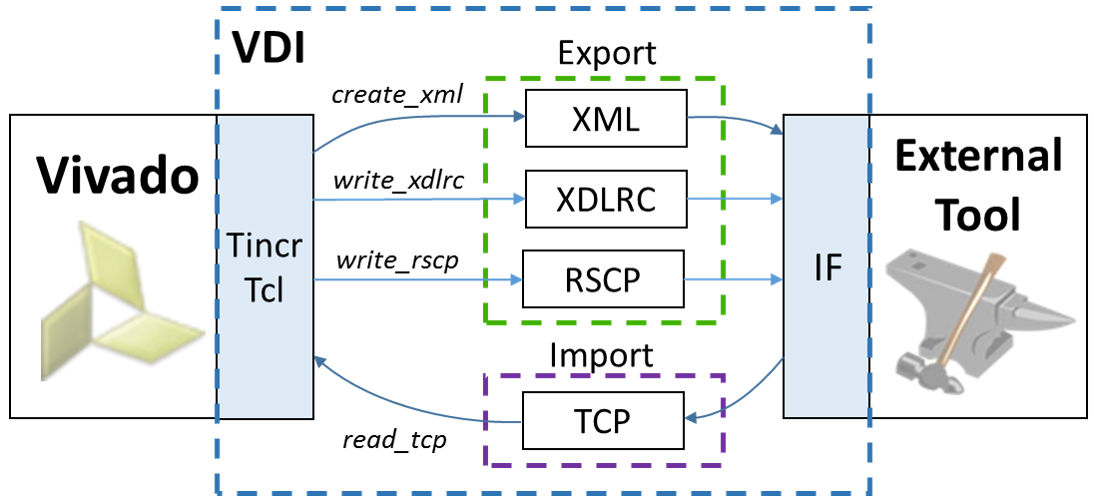
\includegraphics[width=.8\columnwidth]{vdi.png}
 \caption{Components of the Vivado Design Interface (VDI)}
 \label{fig:vdi}
\end{figure}

\subsection{RapidSmith2}

The RapidSmith framework has helped researchers create several different CAD
tools targeting Xilinx devices. Due to the format of XDL however, these CAD
tools always operate at site boundaries. This makes it difficult to explore sub-site CAD
algorithms that work explicitly with sub-site components (i.e. BELs, site PIPs,
etc.) such as packers. Travis Haroldsen was interested in exploring packing
algorithms for Virtex6 devices, and so created RapidSmith2. RapidSmith2 updated
the internal data structures of RapidSmith to the BEL and cell-level, allowing
algorithms to have finer grained control over sub-site placement and routing. 
Because it was originally targeting the Virtex6 architecture, the initial
version of RapidSmith2 took as input a XDL netlist, and \textbf{unpacks} the
netlist to its corresponding cells, nets, BELs, and wires. RapidSmith2 has
since been updated to support Vivado designs exported through VDI (achieving
the original goal of this work). The remainder of this document details
important aspects of RapidSmith2 to help researchers quickly develop
experimental CAD tools for their research.

\subsection{RapidSmith2 Usage Model and Structure}
The usage model for RapidSmith2 is shown in \autoref{fig:UsageModels}.  As can be
seen, a design can be exported from Vivado at multiple different points in the
Vivado design flow through VDI. In each case, Tincr is used to export a
RapidSmith Checkpoint (RSCP)) which can then be imported into RapidSmith2.  At
those same points in the design flow, RapidSmith2 can export a Tincr Checkpoint
(TCP) which can then be imported back into Vivado. Thus, a complete solution
involves Vivado, Tincr, and RapidSmith2.

\begin{figure}[htb]
\centering
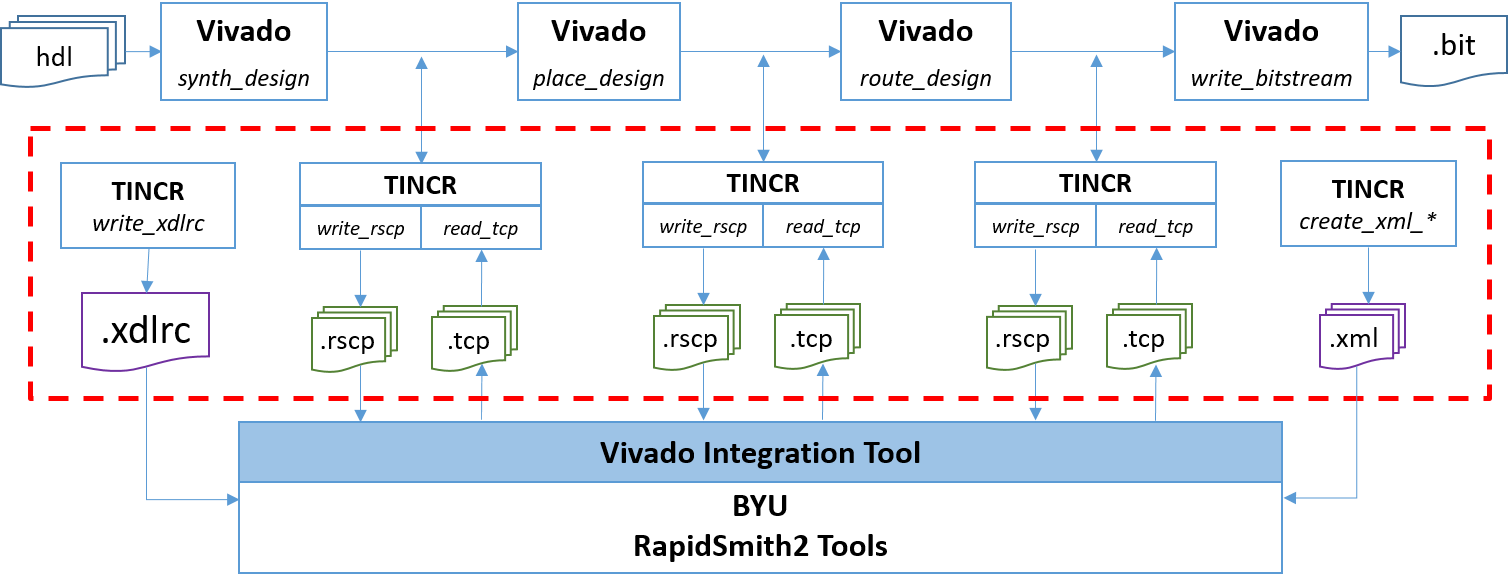
\includegraphics[width=\columnwidth]{usageModel.png}
\caption{Vivado and RapidSmith2 Usage Model}
\label{fig:UsageModels}
\end{figure}

\subsection{Publications and Theses}
Several publications and theses have been accepted as a result of this work.
They are listed here for those who are interested in learning more about RapidSmith2,
\texttt{Tincr}, and VDI.

\begin{enumerate}
  \item B. White. (2014) Tincr: Integrating custom cad tool frameworks with the
  xilinx vivado design suite. [Online]. Available:
  http://scholarsarchive.byu.edu/etd/4338/ ix, 6, 92
  
  \item B. White and B. Nelson, “Tincr A Custom CAD Tool Framework for Vivado,”
  in ReConFigurable Computing and FPGAs (ReConFig), 2014 International
  Conference on. IEEE, Dec. 2014. 3, 12 
   
  \item T. Haroldsen, B. Nelson, and B. Hutchings, “Rapidsmith 2: A framework
  for bel-level cad exploration on xilinx fpgas,” in Proceedings of the 2015
  ACM/SIGDA International Symposium on Field-Programmable Gate Arrays. ACM,
  2015, pp. 66–69. 3, 17
  
  \item  T. Haroldsen, B. Nelson, and B. Hutchings, “Packing a modern xilinx
  fpga using rapidsmith,” in ReConFigurable Computing and FPGAs (ReConFig),
  2016 International Conference on. IEEE, 2016, pp. 1–6. 17
  
  \item T. Townsend and B. Nelson, “Vivado Design Interface: An Export/Import
  Capability for Vivado FPGA Designs ” in Field Programmable Logic and
  Applications (FPL), 2017 27th International Conference.
  
  \item Townsend, Thomas James, "Vivado Design Interface: Enabling CAD-Tool
  Design for Next Generation Xilinx FPGA Devices" (2017). All Theses and
  Dissertations. 6492. http://scholarsarchive.byu.edu/etd/6492 
\end{enumerate}

% \subsection{RapidSmith vs. RapidSmith2}
% \subsubsection{What Was The Original RapidSmith?}
% The original RapidSmith was written by Christopher Lavin as a part of his PhD
% work at BYU.  It was based on the Xilinx Design Language (XDL) which provides a
% human-readable file format equivalent to the Xilinx proprietary Netlist Circuit
% Description (NCD) of ISE.  With RapidSmith, researchers were able to import
% XDL/NCD, manipulate, place, route and export designs among a variety of design
% transformations.  The RapidSmith project made an excellent test bed to try out
% new ideas and algorithms for FPGA CAD research because code could quickly be
% written to take advantage of the APIs available.
% 
% RapidSmith also contained packages which could parse/export bitstreams (at the
% packet level) and represent the frames and configuration blocks in the provided
% data structures.  In this regard, RapidSmith did not include any proprietary
% information about Xilinx FPGAs that is not publicly available.
% 
% RapidSmith continues to be functional and is still available at the
% SourceForge.net website.  There, you will find documentation, installation
% instructions, the RapidSmith code base, and a collection of demo programs based
% on it.
% 
% \subsubsection{What is RapidSmith2?}
% With the announced end of ISE (with the Virtex7 family of parts being the last
% family to be supported by ISE), there was no path forward to newer parts using
% RapidSmith.  This is because XDL is not available with Vivado. With
% Vivado, however, Xilinx has provided an extensive Tcl scripting capability which 
% initially looked as if it could provide a similar capability to that provided by
% XDL in terms of accessing both Vivado's design and device data and in terms of
% creating and modifying Vivado designs.  However, as described above, Vivado's
% Tcl is limited by speed and memory challenges.
% The development of RapidSmith2 consisted of three parts.
% 
% \subsubsection{Tincr: Integrating Custom CAD Tool Frameworks with the Xilinx 
% Vivado Design Suite} \label{sec:tincr}
% 
% In the first part, the Vivado Tcl capability was investigated to ensure that,
% indeed, it did provide the needed ability to access design and device data and
% export that to external tools such as RapidSmith.  This resulted in the Tincr
% project, led by Brad White as a part of his MS work at BYU, with Thomas
% Townsend making additions as a part of his research.
% 
% Tincr is a Tcl-based library of routines which (a) provide a variety of
% functions to simply make working with Vivado via Tcl easier, (b) provide a way
% to export all the data associated with a Vivado design into what is called a
% Tincr Checkpoint (TCP), (c) provide a way to reimport Tincr Checkpoints back
% into Vivado, and (d) access device data from Vivado and output that data in the
% form of XDLRC files (these are the files which XDL used to describe devices and
% are necessary for RapidSmith and RapidSmith2 to understand the structure of and the
% resources available for use in a given Xilinx part).  Tincr is available at 
% \href{https://github.com/byuccl/tincr}{\color{blue}https://github.com/byuccl/tincr}.
% Tincr is described in two publications:
% 
% \begin{quotation}B. White and B. Nelson, "Tincr � A custom CAD tool framework
% for Vivado," 2014 International Conference on ReConFigurable Computing and FPGAs (ReConFig14),
% Cancun, 2014, pp. 1-6, DOI: 10.1109/ReConFig.2014.7032560
% 
% White, Brad S., "Tincr: Integrating Custom CAD Tool Frameworks with
% the Xilinx Vivado Design Suite" (2014), BYU Scholars Archive, Paper 4338. 
% \\URL:http://scholarsarchive.byu.edu/etd/4338
% \end{quotation}
% 
% \subsubsection{RapidSmith2: A Framework for BEL-Level CAD Exploration on Xilinx FPGAs}
% The second part of the development of RapidSmith2 was to add a new layer of design
% representation to RapidSmith which more closely matches that of Vivado.  This
% was done as a part of his PhD work by Travis Haroldsen at BYU.  As of this
% writing, one paper on RapidSmith2 has appeared:
% 
% \begin{quotation}Travis Haroldsen, Brent Nelson, and Brad Hutchings, “RapidSmith
% 2:
% A Framework for BEL-Level CAD Exploration on Xilinx FPGAs�, Proceedings of the
% 2015 ACM/SIGDA International Symposium on Field-Programmable Gate Arrays,
% February 2015, Monterey CA, pp. 66-69, DOI: 10.1145/2684746.2689085.
% \end{quotation}
% 
% \subsubsection{Vivado and RapidSmith2 Integration}
% The third part of the development of RapidSmith2 was to create the ability to export
% designs from Vivado and into RapidSmith2 and, correspondingly, to import RapidSmith2 data back
% into Vivado.  This was completed during 2016, largely by Thomas Townsend
% as an MS student at Brigham Young University.  The initial
% public release of RapidSmith2 was made in January 2017 once that piece was in place.
% 
% \subsubsection{What is All This About XDL and XDLRC and How Does RapidSmith2 Fit Into
% That?} 
% The Xilinx ISE tools had the capability to export XDL and XDLRC files which
% RapidSmith used: 
% \begin{itemize}
%   \item An XDLRC file was a complete description of a given Xilinx FPGA,
%   describing every tile, every switchbox, every wire segment, and every PIP in
%   the part.  RapidSmith was able to process this information and create a device
%   representation for use in support of CAD tools such as placers and routers.
%   \item An XDL file was a textual representation of an NCD file (a user design).
%   It described the user design as a collection of \cls{Instances} and \cls{Nets}. Instances
%   correspond to things like {SLICEs}, {BRAMs}, {DSP48s}, and {IOBs}.  Instances could be
%   placed onto \cls{Sites}. Additionally, Nets in XDL consisted of a list of
%   \cls{Pins} (their logical connections) and an optional list of \cls{PIPs} (their physical
%   routing connections).
% \end{itemize}
% In Vivado, however, designs are described as a collection of \cls{Cells} where a Cell
% corresponds to things like LUTs, flip flops, etc.  A Cell may be placed
% onto a \cls{BEL} object such as an ALUT or a BFF.  RapidSmith2 contains a new layer of
% hierarchy in its design and device descriptions where Cells and BELs are first-class objects and
% design manipulation is all done at the Cell/BEL level.
% 
% Also, Vivado Nets are described using directed routing strings rather than lists
% of PIPs.  RapidSmith2 also contains a set of new classes to enable the representation
% and manipulation of Nets in a format compatible with these routing strings.
% 
% Thus, using RapidSmith2, design manipulation is now done at the level of Cells and BELs
% and importing/exporting designs to/from Vivado is now fully supported.
% 
% \subsection{RapidSmith2 Usage Model and Structure}
% The usage model for RapidSmith2 is shown in \autoref{fig:UsageModels}.  As can be
% seen, a design can be exported from Vivado at multiple different points in the
% Vivado design flow.  In each case, Tincr is used to export a RapidSmith
% Checkpoint (RSCP)) which can then be imported into RapidSmith2.  At those same points in
% the design flow, RapidSmith2 can export a Tincr Checkpoint (TCP) which can then be
% imported back into Vivado.
% Thus, a complete solution involves Vivado, Tincr, and RapidSmith2.
% 
% \begin{figure}[htb]
% \centering
% 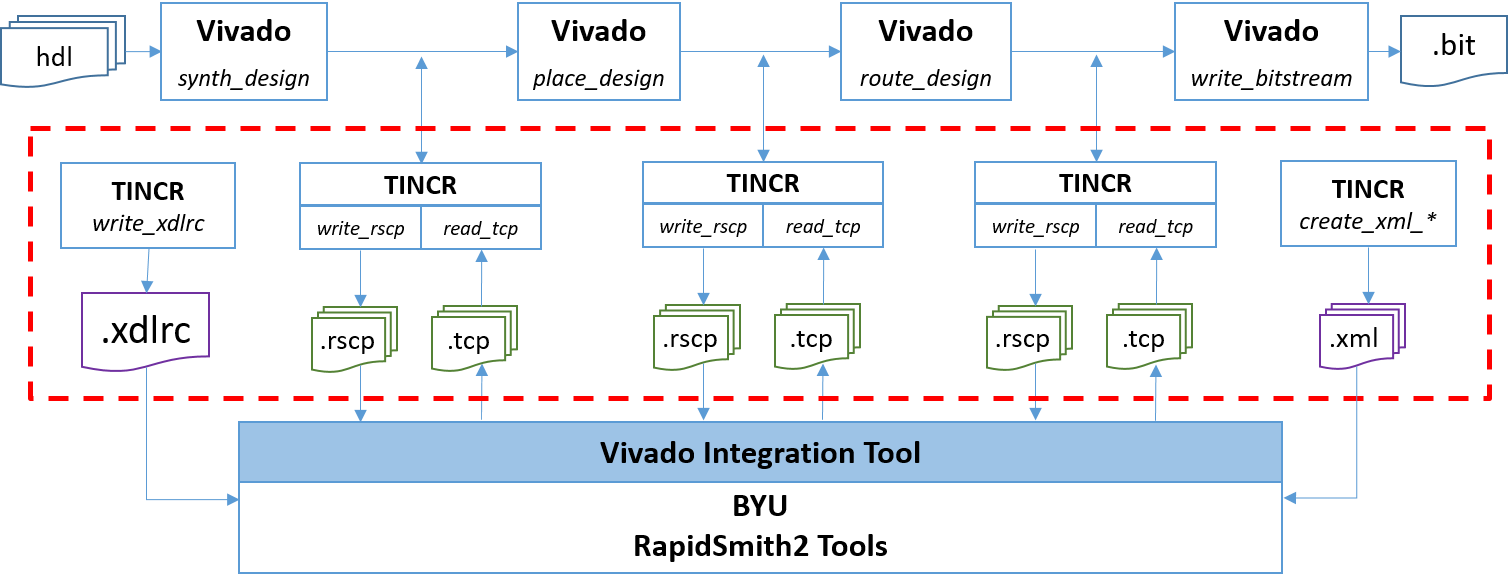
\includegraphics[width=\columnwidth]{usageModel.png}
% \caption{Vivado and RapidSmith2 Usage Model}
% \label{fig:UsageModels}
% \end{figure} 

%%%%%%%%%%%%%%%%%%%%%%%%%%%%%%%%%%%%%%%%%%%%%%%%%%%%%%%%%%%%%%%%%%%%%%%%%%%%
% Section 3: Getting Started
%	This section contains installation instructions for RapidSmith2, and
%	how to test the installation is correct. 
%%%%%%%%%%%%%%%%%%%%%%%%%%%%%%%%%%%%%%%%%%%%%%%%%%%%%%%%%%%%%%%%%%%%%%%%%%%%
\newpage
\section{Getting Started}

\subsection{Installation}

RS2 is available on Github at:
{\color{blue}{\url{https://github.com/byuccl/RapidSmith2}}}.
You can either build RS2 into .class and .jar files for use in any Java
environment, or configure RS2 to work in an IDE (recommended).

\subsubsection{Requirements for Installation and Use}
\begin{itemize}
  \item Windows, Linux or Mac OS X all will work (see additional notes below for
  Mac OS X)
  \item Vivado 2016.2. Later versions of Vivado may work, have not been tested
  yet. Earlier versions will not work.
  \item JDK 1.8 or later
  \item Tincr 
\end{itemize}

Tincr is a companion project
({\color{blue}{\url{https://github.com/byuccl/tincr}}}) which is used for
importing/exporting designs between Vivado and RS2.  For getting started (running the example programs on the provided sample designs) you will not need it installed.
Later, as you  actually start processing your own Vivado designs you will need
to obtain and install it. There are additional dependencies beyond these
required for installation, but they are either provided in the distribution
itself or are automatically retrieved for you as a part of the installation process. 
Examples of these additional dependencies include QT Jambi and the BYU Edif
Tools.
 
\subsubsection{Steps for Installation}

\begin{enumerate}
  \item Clone the RS2 repository at
  {\color{blue}{\url{https://github.com/byuccl/RapidSmith2}}}. If you are not
  familiar with GitHub, you will need to install Git on your computer, and run the
  following command in an open terminal: 
\vspace{-0.07in}
\begin{code}
git clone https://github.com/byuccl/RapidSmith2
\end{code} 
  \noindent This will copy the RS2 repository into a local directory.
  \item Create a new environment variable called RAPIDSMITH\_PATH, and point it
  to your local repository of RS2 that you setup in step (1). This is needed so
  RS2 can find required device files and other items at runtime.
  \item Build the  RS2 project. RS2 is managed using a gradle build system.
  To build the project, navigate to your local repository of RS2 and execute one
  of the following scripts in a terminal:
  \begin{code}
	gradlew build (unix)
	gradlew.bat build (windows)
  \end{code}
  The build process could take a few minutes.
  \item At this point, you have two choices: set up RS2 for use in an IDE, or
  run RS2 from the command line. Both choices are detailed below.
  \paragraph{Running from an IDE} The gradle scripts in RS2 currently support
  setup for both Eclipse and IDEA Java IDEs. This section will detail how to
  setup the Eclipse environment, but similar steps can be taken for IDEA. If
  using Eclipse, it is best to use version Eclipse Neon or later. To create a
  new eclipse project, execute one of the following in a terminal:
  \begin{code}
	gradlew antlr eclipse (unix)       
	gradlew.bat antlr eclipse (windows)
  \end{code}
  Executing these will create an Eclipse \fil{.project} file. After the project
  file has been created, you can import the project into Eclipse by opening
  Eclipse and selecting:
  \begin{code}
	File->Open Projects From File System 
  \end{code}
  and pointing it to your RS2 local repository. All Java source files
  will be found under \dir{src/main/java}. \pgm{NOTE:} Your RS2 git repository
  should not be put inside your eclipse workspace. It is better to put it
  elsewhere, and then import it into your workspace.
  \paragraph{Building on the Command Line} After step (3) in the installation
  process, gradlew produces everything that you will need to run RS2 from the
  command line. The following directories are created: 
  \begin{itemize}
    \item \fil{build/classes/main}: This folder contains the RS2 class file
    directory tree.
    \item \fil{build/libs}: This folder contains a Jar file of the RS2 class
    files.
    \item \fil{build/distributions}: This folder has both .zip and .tar files
    with contains all Jars needed to run RS2 from the command line. This
    includes a full jar of the RS2 build alond with copies of dependency Jars
    (such as QT-Jambi).
  \end{itemize} 
  After adding the appropriate .class files or Jars to your \texttt{CLASSPATH},
  you should be able to run RS2 tools from the command line. If you make any
  changes to the RS2 code, you will have to rebuild before running the program
  again (Step 3). \pgm{CAUTION:} An obvious thing to try is to mix and match
  developing in Eclipse but then running the resulting apps from the command
  line. Just be aware that Eclipse puts its compiled .class files in very
  different places than where the gradle build process puts its .class and
  .jar files. Make sure you understand that before you try to combine these two
  build/execution methods. Our suggested approach is to choose one or the
  other, but not both.
\end{enumerate}

\subsubsection{Alternative Installation and Use}

RS2 is also available as a Docker container. To painlessly set up a working RS2 environment, type:
\vspace{-0.05in}
\begin{code}
docker run -it byuccl/rapidsmith2
\end{code}
\vspace{0.04in}
For more information about Docker, see the \href{https://docs.docker.com/engine/getstarted/}{\color{blue}guide}.

\subsubsection{Additional Notes for Mac OS X Installation}

The instructions above require you to set the \env{RAPIDSMITH\_PATH}
environment variable.  If running from the command line, the environment
variables can be added to your \fil{.bash\_profile} file as in any other
UNIX-like system.  However, if using an IDE such as Eclipse you either need to
define the environment variable for every Run Configuration you create, or you
need to add the \env{RAPIDSMITH\_PATH} definition system-wide in OS X. This can
be done, but how to do so differs based on what OS X version you are running
(and seems to have changed a number of times over the years). Search the web for
instructions for how to do so if you desire. \pgm{Hint}: you will likely have
to edit some \fil{.plist} files.

\subsubsection{Running RS2 Programs}
Some points to keep in mind while configuring and running RS2 programs:
\begin{itemize}
  \item The RS2 code base contains a number of assertions which may be helpful  
  as you are developing code.  These are not enabled by default in Java.  To
  enable them, add \opt{-ea} as a VM argument.  This is highly recommended.
  \item If you are running on a Mac, when running RS2 programs that use Qt  (any
  of the built-in programs like \pgm{DeviceBrowser}) that are GUI-based, you
  will need to supply an extra JVM switch, \opt{-XstartOnFirstThread}.
  \item A common error when running RS2 programs is failing to have your
  \env{RAPIDSMITH\_PATH} defined.  If this is the case when you try to execute a
  program, an \texttt{EnvironmentException} will be thrown telling you that you
  forgot to set the variable.
  \item If you are running on Windows, only a 32-bit QT Jar file is included in
  the RS2 repository. This means that you will need to set your JRE to a 32-bit
  version when running the GUI programs. We are working on updating QT to the
  latest version, so this will no longer be an issue.
  \item For Linux command line usage, the \env{CLASSPATH} environment variable
  must point to both the full (uncompressed) RS2 jar in the \dir{build/distributions}
  folder as well as all the jar files in the \dir{/lib} subdirectory. An example
  \env{CLASSPATH} could look like this:
  \vspace{-0.15in}  \begin{code}
  �  �  � RAPIDSMITH2-SNAPSHOT/*:RAPIDSMITH2-SNAPSHOT/lib/*
  \end{code}
\end{itemize}

\subsubsection{Testing Your Installation}
\noindent At this point you can test your installation by executing the java
\pgm{DeviceBrowser} program: 
\begin{code}
java edu.byu.ece.rapidSmith.device.browser.DeviceBrowser
\end{code} \vspace{0.1in}    

\noindent This can be done either from within Eclipse or from the command line,
depending on how you are running RS2 (if running under OS X be sure to provide the
\opt{-XstartOnFirstThread JVM argument}. If all goes well you should see a
graphical representation showing the details of a physical FPGA device as shown
in \autoref{fig:deviceBrowser}.  You may initially be zoomed far in and might
want to zoom out to see the entire chip layout.

\begin{figure}[H]
\centering
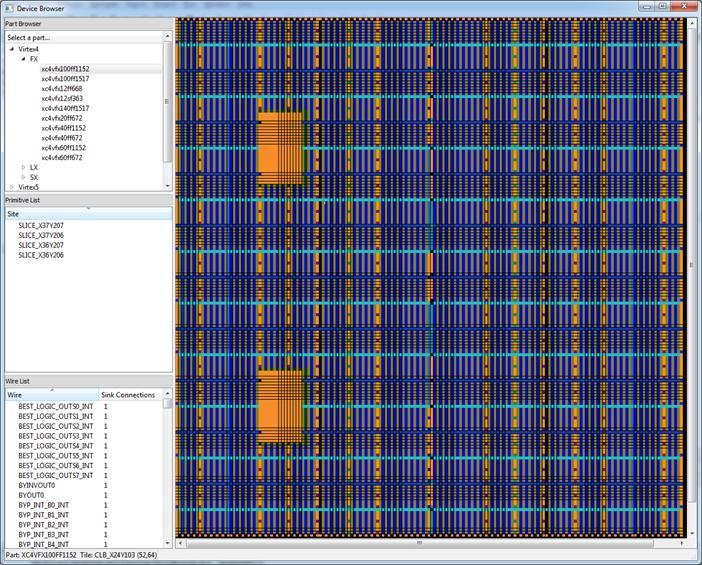
\includegraphics[width=0.8\columnwidth]{deviceBrowser}
\caption{\pgm{DeviceBrowser} Sample Display}
\label{fig:deviceBrowser}
\end{figure}

\subsection{Running Real Designs - An Overview}
This section will lead you through running an entire design from Vivado through
RS2 and back.  In this example you will fully synthesize and implement a
complete design in Vivado and then move it into RS2.  However, later as you gain
experience you may choose to only synthesize  designs before exporting
them to RS2 or you may choose to export and work with Vivado Out-Of-Context
(OOC) Checkpoints.

The steps to be covered include:

\begin{enumerate}
  \item Synthesize, place and route a design in Vivado
  \item  Export the design from Vivado in the form of an RSCP (RapidSmith
  Checkpoint)
  \item Import the RSCP  into RS2
  \item Run some analysis on the design
  \item Export the design from RS2 as a TCP (Tincr Checkpoint)
  \item Import the TCP back into Vivado
\end{enumerate}

In a real CAD flow you would likely do something more interesting
than the analysis in Step 4 above, but this overview is intended to help you
through the Vivado-to-RS2-back-to process so you can get started.

Note: the entire flow requires the installation of Tincr as well as RS2 so if
you skipped the Tincr installation above, go and install it now.

\subsubsection{Synthesize, Place, and Route a Design in Vivado and Then Export
It As a RSCP} If you desire, you may do this step any way you are used to using
Vivado (with or without using the Vivado GUI for example).  In this step, we
will do it using the Vivado Tcl interface.

First, start up Vivado in command line mode.  This can be done using the
``Vivado Tcl Shell'' program item or by executing ``vivado -mode tcl''.  Once
the shell has started up, you may execute the following:
                
\begin{lstlisting}
	Vivado\% cd <path to directory containing your HDL files>
	Vivado\% link_design -part xc7a100t-csg324-3
	Vivado\% read_verilog [glob *.v]
	Vivado\% synth_design -top myTopLevelEntityName -flatten_hierarchy full 
	Vivado\% place_design
	Vivado\% route_design
	Vivado\% package require tincr
	Vivado\% tincr::write_rscp myTopLevelEntityName
	Vivado\% close_project
\end{lstlisting}
Most of the above commands should be self-explanatory and can be adapted to
compile VHDL or SystemVerilog files.
Importantly,  you must flatten the design hierarchy when running
the synthesis step as shown above.  The result of executing this will be a new
directory which contains the RapidSmith Checkpoint.

As already mentioned, this shows how to create a fully placed and routed design
in Vivado prior to export.  There is no requirement, however, that the design is
either placed or routed prior to export.  You may choose to export it any time
after it has been synthesized.

Finally, note that a set of sample HDL designs are provided in the RS2
distribution (in \dir{exampleVivadoDesigns}) and which you could use for your
learning.
You can read about them as well as a script which implements a version of the
above compilation steps in Section~\ref{sampledesigns} of this report.  Note
that the compilation script described there expects a particular directory
structure to hold your source files.  Otherwise, the script implements 
essentially what is shown above.

\subsubsection{Import the RSCP into RS2}
Once you have a RSCP you are ready to create a Java program for RS2 that will be
able to import that RSCP into RS2 so you can do something with it.

As described in Section~\ref{examples} of this report (and
Section~\ref{sec:importExportExample} in particular) a sample import/export program
is provided in the RS2 distribution which illustrates how to import
and export designs from RS2.  This program, when run, will read in a
RapidSmith Checkpoint (RSCP), walk the resulting data structures and
then prettyprint the design contents, and then write out the
corresponding Tincr Checkpoint.   

You should examine the code for that
program to understand its operation and the subroutine calls that can
be used to do those steps.  The net result from running that program
is to export a Tincr Checkpoint, stored in a directory with a ``tcp'' extension.

\subsubsection{Importing a Tincr Checkpoint Back into Vivado}
At this point you can import the resulting Tincr Checkpoint back into Vivado. 
Assuming the original RSCP was ``add.rscp'', after running the import/export
example program  you will have a ``add.rscp.tcp'' directory.  After starting
Vivado up in Tcl mode (``vivado -mode tcl'') you can execute the following
commands to import the checkpoint:

\vspace{-0.15in}  \begin{code}
	Vivado\% cd <path to directory containing your add.rscp.tcp directory>
	Vivado\% package require tincr
	Vivado\% tincr::read_tcp add.rscp.tcp
	Vivado\% start_gui
\end{code}

At this point the Vivado GUI will open and you will see that there are cells and
nets associated with this design.  If you want to save the imported design for
later you could also do the following command:

\vspace{-0.15in}  \begin{code}
	Vivado\% write_checkpoint -force add.dcp
\end{code}

You could then later re-load that into Vivado using the following commands from
the Tcl window:

\vspace{-0.15in}  \begin{code}
	Vivado\% link_design -part xc7a100t-csg324-3
	Vivado\% open_checkpoint add.dcp
\end{code}

You will notice that these instructions focus on running Vivado in Tcl mode to
do all the commands given.  The Vivado GUI is then started once the
commands have executed.  Why not just always run in GUI mode since those same
commands could have been typed into the command window in the GUI? It turns out
that running commands such as these while the GUI window is open makes them run
many times slower than if they were run just in Tcl mode.  So, a typical use
case you might find helpful is to always start Vivado in Tcl mode, do the
commands needed to export or import things, and then open the GUI (using
``start\_gui'') and close the GUI (using ``stop\_gui'') as needed.



%%%%%%%%%%%%%%%%%%%%%%%%%%%%%%%%%%%%%%%%%%%%%%%%%%%%%%%%%%%%%%%%%%%%%%%%%%%%%%%%%%%%%%%%%
% Section 4: Xilinx Devices
%	This section contains a description of the following:
%	- Vivado FPGA devices (with terminology)
%	- Device data structures in RapidSmith, 
%	- Device files and XDLRC files  
%	- Step-by-step guide on how to intall new devices  
%%%%%%%%%%%%%%%%%%%%%%%%%%%%%%%%%%%%%%%%%%%%%%%%%%%%%%%%%%%%%%%%%%%%%%%%%%%%%%%%%%%%%%%%%
\newpage
\section{Devices}
\graphicspath{{./techReportFigures/sec4_devices/}}

%%%%%%%%%%%%%%%%%%%%%%%%%%%%%%%%%%%%%%%%%%%%%%%%%%%%
% 	Xilinx FPGA Architecture
%%%%%%%%%%%%%%%%%%%%%%%%%%%%%%%%%%%%%%%%%%%%%%%%%%%%
\subsection{Xilinx FPGA Architecture Overview} \label{fpgaArch}
This section is intended to give a brief introduction to Xilinx FPGA
architecture and terminology. The terminology introduced here is consistent
with the terminolgy used in the Vivado Design Suite. If you are already familiar
with Xilinx FPGA devices, then you can skip to \autoref{devicesRS2}. 
As you read through this section, it may be helpful to open a sample device in Vivado's
Device Browser. To do this, open a new command prompt and run Vivado in Tcl mode
(``vivado -mode tcl''). Then, run the following commands in the Vivado prompt:

\begin{lstlisting} [numbers=none,keywordstyle=\ttfamily]
Vivado% link_design -part xc7a100tcsg324-3 -quiet
Vivado% start_gui
\end{lstlisting}

\noindent
Replace ``xc7a100tcsg324-3" with any Xilinx part you are interested in looking
at. After these commands are run, a GUI view should pop up showing the
components of an Artix7 FPGA part. Use this to explore the Xilinx device 
architecture if needed.

% Device Hierarchy
\subsubsection{Device Hierarchy} \label{sec:deviceHierarchy}
Xilinx FPGAs can be broken down into \texttt{series},
\texttt{families}, and individual \texttt{parts}. At the highest level, a series
defines a unique FPGA architecture. Vivado currently supports three different
series: Series7, UltraScale, and UltraScale+. As shown in
\autoref{tab:vivadoFamilies}, each series can be broken down into a list of
families. These families all use the same series architecture, but are
optimized for cost, power, performance, size, or another metric.

\begin{table} [h!]
\caption{Vivado Device Families (organized by series)}
\label{tab:vivadoFamilies}
\vspace{-.15in}
\begin{center}
\begin{tabu}{ |c|c|c|c| }
\hline
\textbf{Series7} & \textbf{UltraScale} & \textbf{UltraScale+} \\
\hline
\hline
 Kintex & Kintex & Kintex \\
 Virtex & Virtex & Virtex \\
 Artix &  &  \\
 Spartan &  &  \\
 Zynq &  &  \\ 
\hline
\end{tabu}
\end{center}
\end{table}

\begin{figure}[b!]
 \centering
 \includegraphics[width=\columnwidth]{deviceHierarchy.png}
 \caption{Xilinx Device Hierarchy}
 \label{fig:deviceHierarchy}
\end{figure}

\noindent Families can further be broken down into one or more parts (actual
FPGA devices). A Xilinx part has a variety of attributes including its number,
package type, and speed-grade. Take the part ``xcku025-ffva1156-1-c'' as an
example. This part is within the Kintex UltraScale family, uses a ``ffva1156''
package type, and has a speed grade of ``1-c''. \autoref{fig:deviceHierarchy}
shows the device hierarchy of a Xilinx part . The following subsections describe
each internal component of a Xilinx FPGA as shown in the figure.

% Tiles
\subsubsection{Tiles}
A Xilinx FPGA is organized into a two-dimensional array of \texttt{Tile}s. Each
tile is a rectangular component of a device that performs a specific function
such as implementing digital logic or storing BRAM memory. Tiles are stamped
across a device  and wired together through the general routing fabric. All
copies of a tile type are identical or nearly identical (they may have minor
routing differences). \autoref{fig:tileExample} displays three types of tiles
in an Artix7 device. The \textbf{VBRK} tile on the left is used for wiring
signals between other tiles (these connections are not programmable). The 
\textbf{INT\_L} tile on the right is a switchbox tile. These are
reconfigurable routing tiles that allow a single wire to be routed to various
locations within the FPGA. The \textbf{CLBLL} tile in the middle is used
to implement combinational and sequential digital logic, and is the fundamental
component of Xilinx FPGAs. Other tile types include DSP, BRAM, FIFO, and IOB.

\begin{figure}[t!]
 \centering
 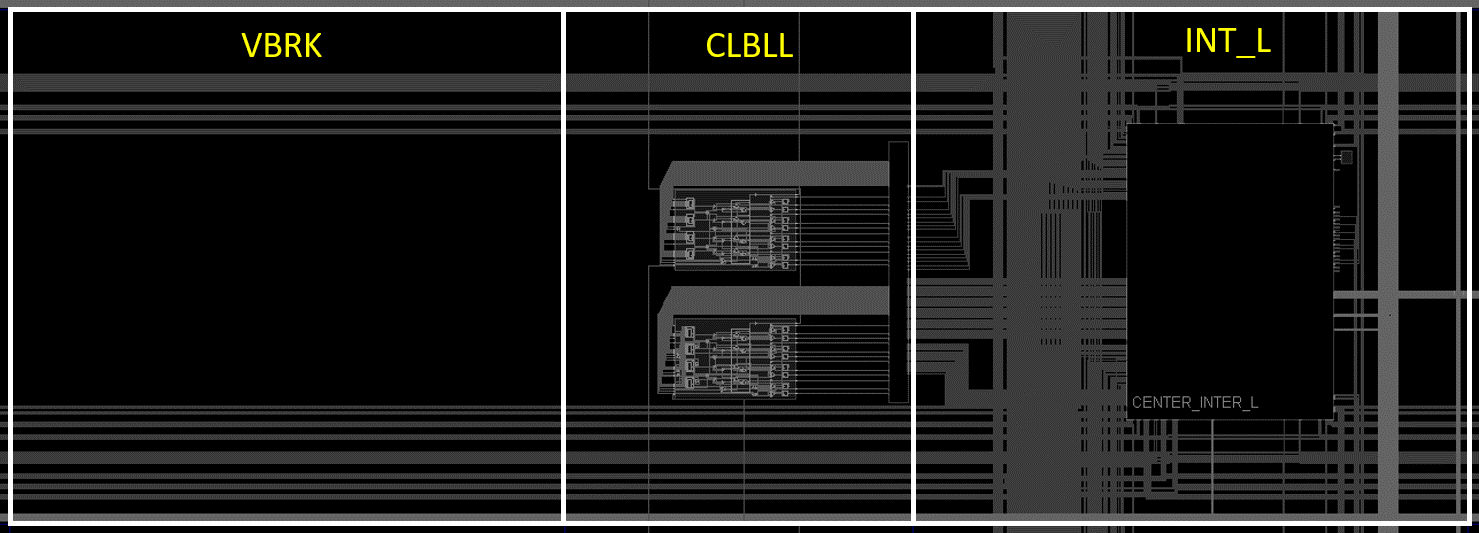
\includegraphics[width=\columnwidth]{tiles.png}
 \caption{Artix7 Tiles}
 \label{fig:tileExample}
\end{figure}

% Sites
\subsubsection{Sites}
Tiles generally consist of one or more \texttt{Site} objects, which organize
the hardware components of the tile into related groups. Specifically, sites are
the part of a tile which perform the tile's ``useful'' function. The remainder
of the tile is used to wire signals to and from its corresponding sites.
\autoref{fig:site} shows an example site of type SLICEL within a Series7 CLBLL
tile. As the figure shows, a site consists of three main components which are
connected through wires:

\begin{figure}[p!]
\centering
   \begin{subfigure}[h!]{0.85\textwidth}
   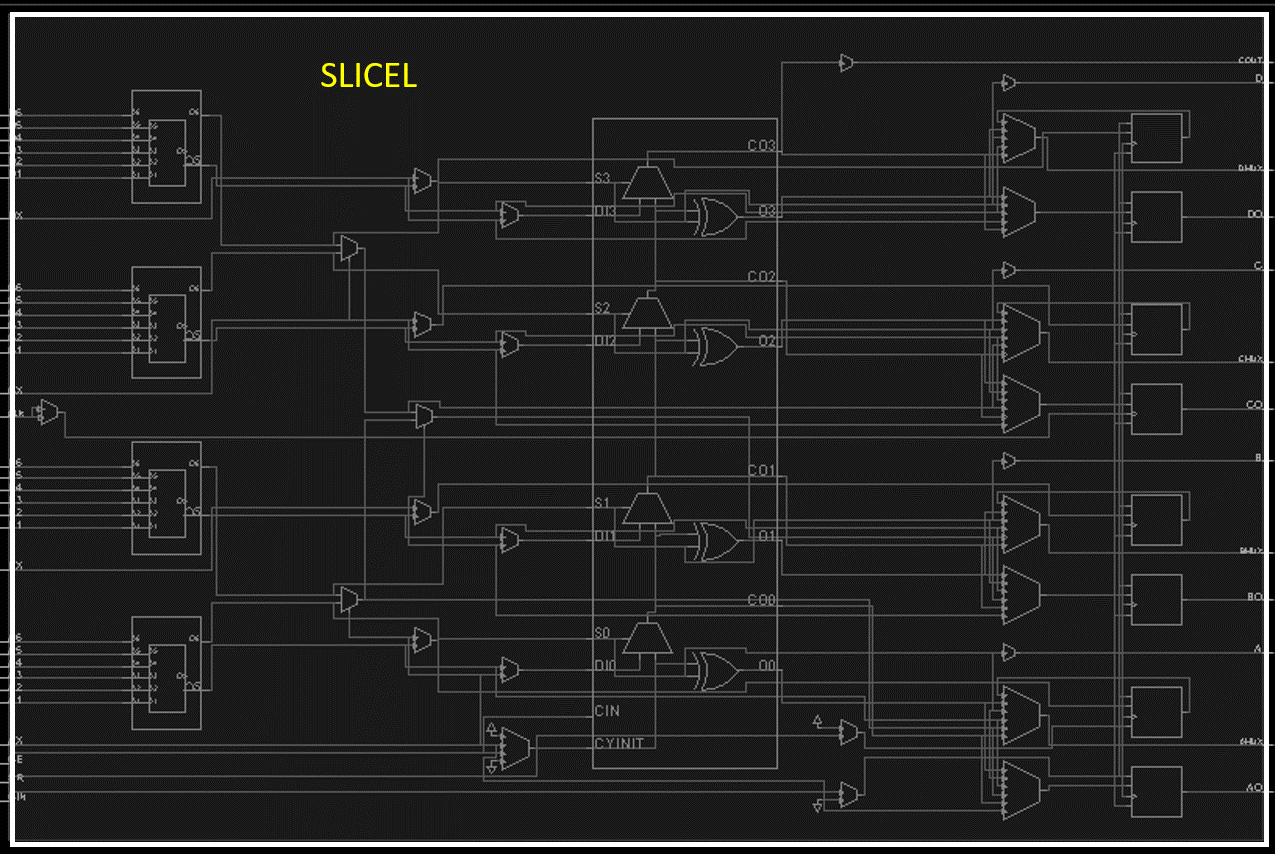
\includegraphics[width=\textwidth]{site.png}
   \caption{}
   \label{fig:site1}
\end{subfigure}

\begin{subfigure}[h!]{0.85\textwidth}
   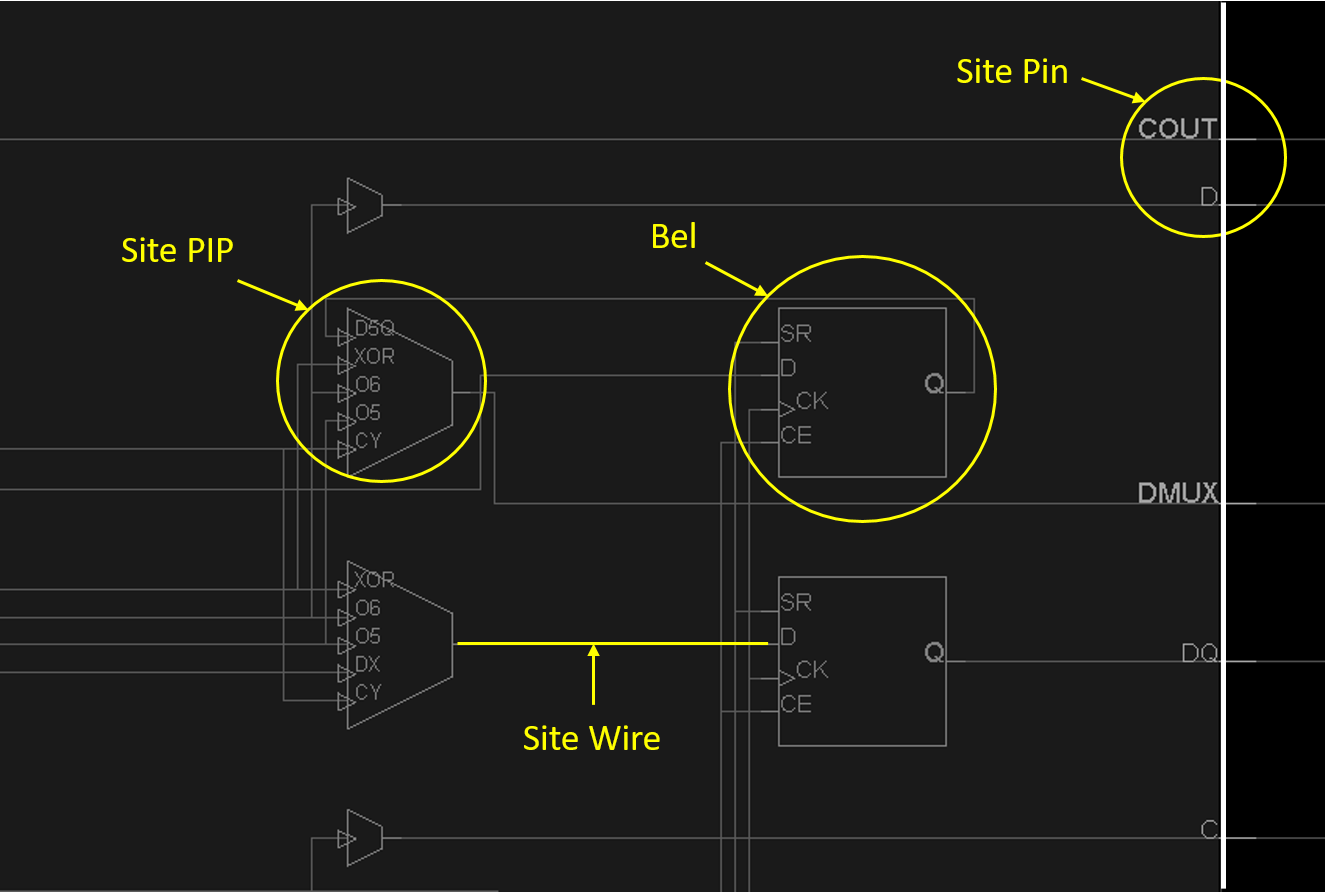
\includegraphics[width=\textwidth]{subsite2.png}
   \caption{}
   \label{fig:site2}
\end{subfigure}

\caption{Series7 SLICEL Site (a), and Highlighted Site Components (b)}
\label{fig:site}
\end{figure}

\begin{itemize}
  \item \textbf{Site} \textbf{PIP}s: Also called routing muxes, these are
  reconfigurable routing PIPs used to specify the internal routing of a site.
  In Vivado, site PIPs are usually configured automatically as cells in a
  design are placed (based on cell properties and placement locations).
  
  \item \textbf{BEL}s: \textbf{B}asic \textbf{EL}ements are hardware components
  within a site for implementing digital logic. For example, look-up-tables
  (LUT) within a SLICEL are used to implement logic equations, and flip-flops
  (FF) are used as storage. In a synthesized netlist, design elements are
  mapped to BELs during implementation.
   
  \item \textbf{Site Pin}s: These pins are connected to wires of the parent tile
  and typically drive/receive signals from the general fabric.
\end{itemize}

\subsubsection{Wires and PIPs} \label{wireSection}
 
\begin{figure}[t!]
	\centering
	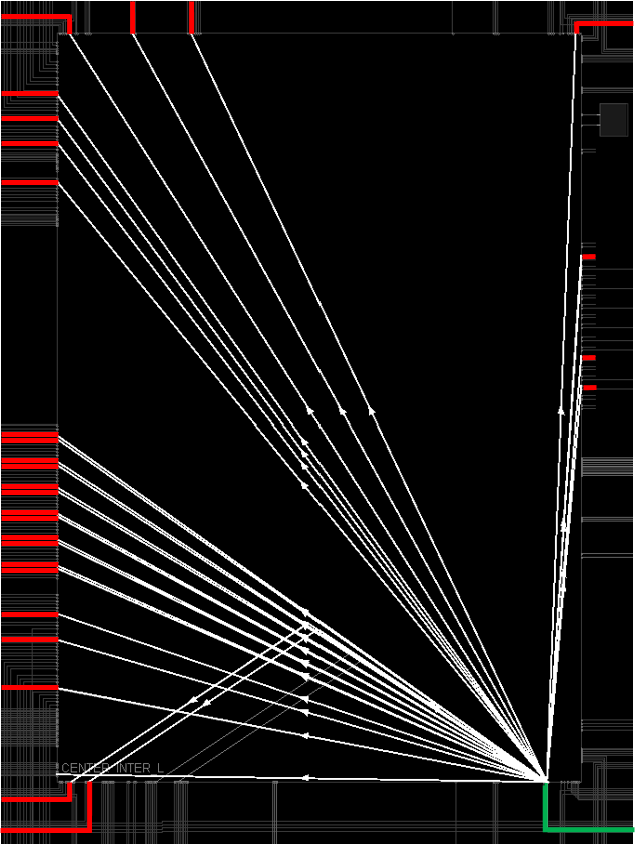
\includegraphics[width=0.65\columnwidth]{pipExample.pdf}
	\caption{An example switchbox tile. The green wire represents a source wire,
	and the red wires represent all possible sink wires in the switchbox. The
	highlighed white sections of the figure are PIP connections.}
	\label{fig:switchboxPIP}
\end{figure} 
 
FPGA components are connected together using metal \texttt{Wire}s (called
\texttt{Node}s in Vivado). To make the FPGA reconfigurable,
wires are connected through programmable interconnect points
(PIPs). Individual PIPs can be enabled or disabled as a design is
being routed, and a string of enabled PIPs uniquely identify the
used wires of a physical route. PIPs are most commonly
found in switchbox tiles, and enable a single wire to be
routed to several locations on the chip. \autoref{fig:switchboxPIP}
shows an example switchbox with its corresponding PIPs. The red wires
represent all downhill nodes that the green wire can connect to through a PIP
connection.

%%%%%%%%%%%%%%%%%%%%%%%%%%%%%%%%%%%%%%%%%%%%%%%%%%%%
% 	Device Data Structures
%%%%%%%%%%%%%%%%%%%%%%%%%%%%%%%%%%%%%%%%%%%%%%%%%%%% 
\subsection{Device Data Structures} \label{devicesRS2}
In the original RapidSmith, the device architecture stopped at the
site level. A site was considered a black box who could be
configured using string attributes, but the actual internal components were
unknown. RapidSmith2 extends the device architecture to include all
components \textbf{within} a site as well. \autoref{fig:deviceDataStructures}
shows the new data structure hierarchy, which can be found in the package \emph{
edu.byu.ece.rapidSmith.device}. The classes and interfaces within
\emph{edu.byu.ece.rapid\-Smith.device} are named to reflect the terminology
used by Xilinx. Many classes that exist in Vivado's Tcl interface have a direct map
to a class in RapidSmith2 (such as a \texttt{Tile}). Because of this, most
RapidSmith2 data structures represent a straightforward part of a Xilinx FPGA.
The \texttt{DeviceBrowser} and \texttt{DeviceAnalyzer} example programs
illustrate how to load and browse a device with \texttt{Tile} and \texttt{Site}
data structures, and \autoref{lst:deviceCalls} shows basic device usage in
RapidSmith2. The remainder of this section details important aspects of
RapidSmith2 devices.

% TODO: update this figure to include package pins
\begin{figure}[t]
	\centering
	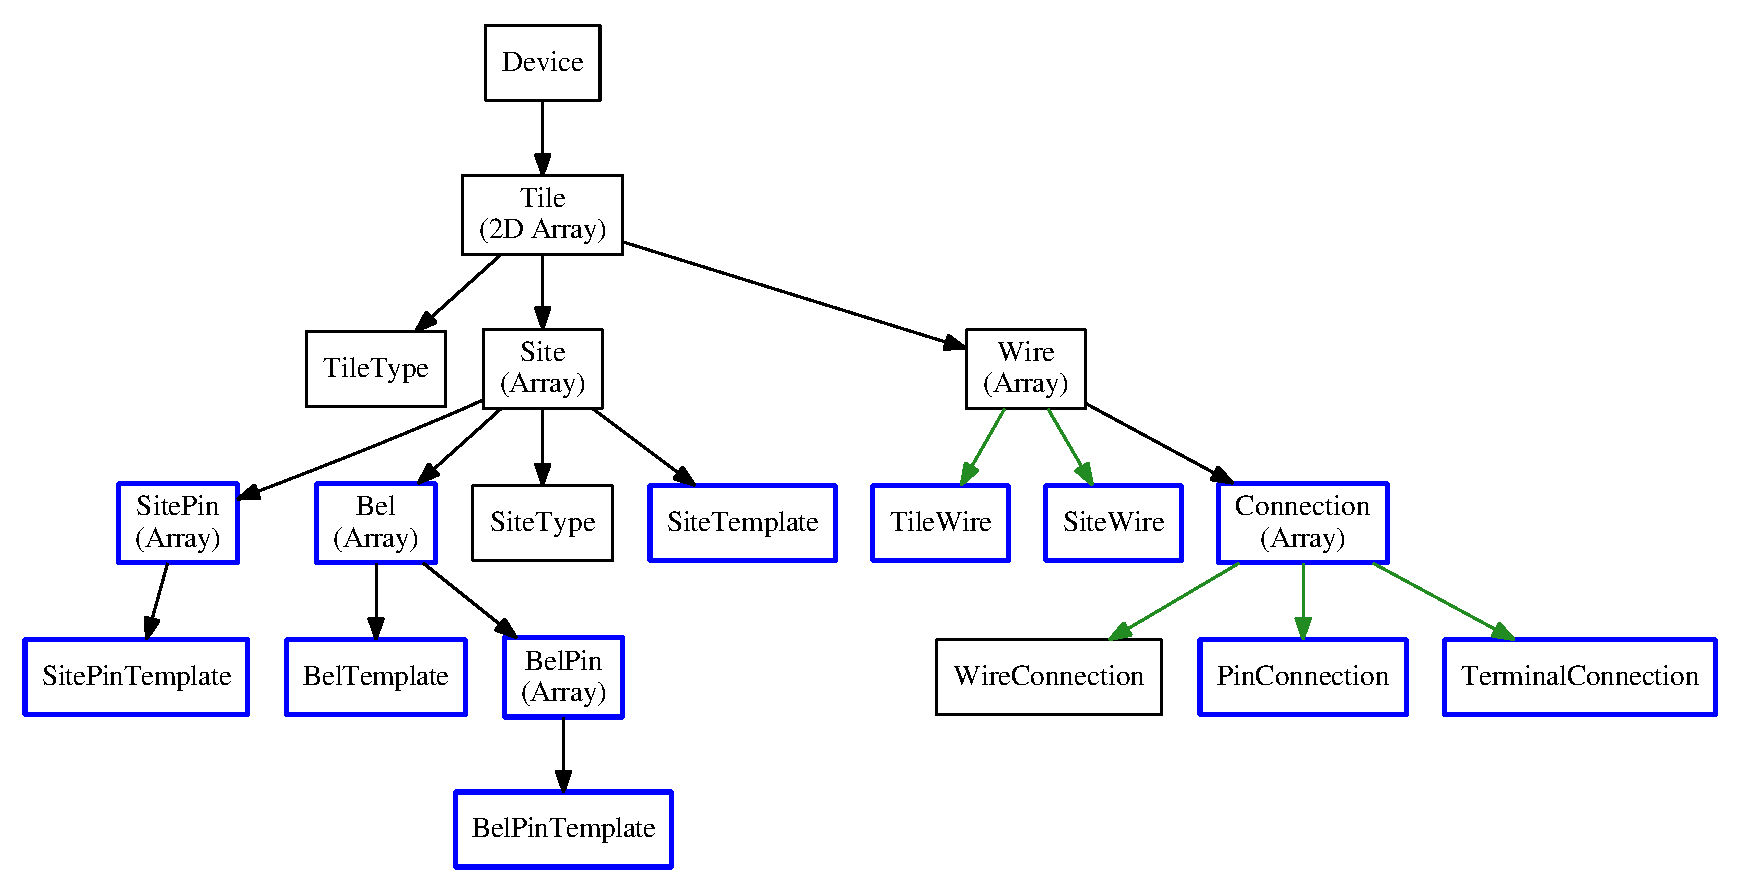
\includegraphics[width=1\columnwidth]{deviceDS.eps}
	\caption{RapidSmith2 Device data structure tree. Green arrows
	represent inheritance, and black arrows represent association. Classes and Interfaces
	bolded in blue are new to RapidSmith 2.}
	\label{fig:deviceDataStructures}
\end{figure}

\begin{lstlisting}[xleftmargin=1.5em, framexleftmargin=1.5em, caption=Basic
device function calls, label=lst:deviceCalls]
  // Get a handle to a device 
  Device device = Device.getInstance("xc7a100tcsg324-3");
	
  // Get device components by name
  Tile tile = device.getTile("CLBLL_R_X27Y130");
  Site site = tile.getSite("SLICE_X44Y130");
  Bel bel = site.getBel("D6LUT");
	
  // Get all device components
  device.getTiles();
  tile.getSites();
  site.getBels();
\end{lstlisting}

\subsubsection{Templates}
As \autoref{fig:deviceDataStructures} shows, there are several template
classes in RapidSmith2. Template classes are used to specify the configuration
of a device structure only once, where the configuration can be reused
across identical objects. The usefulness of templates is best shown with an
example. In an Artix-7 \emph{xc7a100tcsg324} part, there are 11,100 sites of
type SLICEL. Each of these SLICELs have 215 internal components (BELs, pins,
and PIPs). To save memory, RapidSmith2 lazily creates site objects
based on the template only when a handle to a SLICEL site is requested. The
alternative would be to create each of the objects when a device is loaded, but
this would require more memory. Template classes should generally not be
used by the regular user. When creating algorithms using RapidSmith's API, use
the non-template version of classes instead.

\subsubsection{WireEnumerator} \label{wireEnum}
Wires with the same name and function can occur several times throughout a
Xilinx FPGA. For example, the wire \texttt{CLBLL\-\_L\_C2} exists in every tile
of type \texttt{CLBLL\_L} in a Series7 device. To make RapidSmith2
device files small, each uniquely named wire is assigned an integer enumeration
and stored in a \texttt{WireEnumerator} class. The \texttt{WireEnum\-erator}
has methods to convert an integer to the corresponding string wire name and
vice versa.

In previous versions of RapidSmith, the \texttt{WireEnumerator} was used
extensively while building CAD tools. RapidSmith2 has changed this, largely
abstracting the \texttt{WireEnumerator} away in favor of more convenient
methods that return \texttt{Wire} objects which contain a wire's integer
enumeration and name. For example, the name or enumeration of a wire can now be
obtained with the function calls in the \texttt{Wire} interface
\texttt{getWireName()} and \texttt{getWireEnum()} respectively. A handle to the
\texttt{WireEnumerator} still exists in the \texttt{Device} class for those who
want to use it, but this is not recommended.

% TODO: add a code segment here showing the old way vs. new way?

\subsubsection{TileWire and SiteWire} \label{wires}
Wires in RapidSmith2 are uniquely identified not only by their name
(or enumeration), but also by the tile or site in which they exist.
RapidSmith2 introduces the \texttt{TileWire} and \texttt{SiteWire} classes to
encapsulate this information for the user. Many functions in RapidSmith2 now
return a \texttt{TileWire} or \texttt{SiteWire} object (wrapped in a generic
\texttt{Wire}) instead of an integer wire enumeration. \texttt{Wire}s are
connected through \texttt{Connection} objects as described in
\autoref{sec:routing}.

\subsubsection{Package Pins}

Vivado maps all \textit{bonded} IOB sites to corresponding package pins.
Top-level ports of a design can be mapped to these package pins to communicate
with external components. A RapidSmith2 \texttt{Device} object represents Vivado
package pins with \texttt{PackagePin} objects. Each \texttt{PackagePin} 
contains (1) the name of the package pin (i.e. M17), (2) the PAD BEL of the
package pin, and (3) a boolean flag to mark clock package pins. Clock
package pins are those that can access the global clock routing structure of
the FPGA for low skew signals. \autoref{lst:packagePins} shows some available
package pin method calls.

\begin{lstlisting}[xleftmargin=1.5em, framexleftmargin=1.5em,caption=RapidSmith2
package pin functions, label=lst:packagePins] 
  // Get a list of all package pins 
  device.getPackagePins();
	
  // Get a list of clock package pins
  device.getClockPads();
	
  // Get an individual package pin based on the BEL
  Bel bel = device.getSite("IOB_X0Y10").getBel("PAD");
  PackagePin pin = device.getPackagePin(bel);
	
  // Package pin functions
  pin.getName();
  pin.getSite();
  pin.getBel();
  pin.isClockPad();	
\end{lstlisting}

%%%%%%%%%%%%%%%%%%%%%%%%%%%%%%%%%%%%%%%%%%%%%%%%%%%%
% 	Loading a Device
%%%%%%%%%%%%%%%%%%%%%%%%%%%%%%%%%%%%%%%%%%%%%%%%%%%%
\subsection{Loading a Device} \label{sec:loadingDevice}
\autoref{code:loadDevice} below demonstrates how to load a supported device
into RapidSmith2.  The first function call will only load the device into memory
if it has not yet been loaded. If it has been loaded, then the cached
\texttt{Device} data structure will be returned. The second function call will
reload the device from disk, creating a separate \texttt{Device} data
structure. 

\begin{lstlisting}[xleftmargin=1.5em, framexleftmargin=1.5em, caption=Loading a
Device, label=code:loadDevice] 
Device device = RSEnvironment.defaultEnv().getDevice("xc7a100tcsg324");
//or
Device reload = RSEnvironment.defaultEnv().getDevice("xc7a100tcsg324", true);
\end{lstlisting}

\noindent This is useful when implementing multi-threaded code that targets
the same part. \textbf{NOTE:} When a Vivado design is loaded into RapidSmith2
via a RSCP, the corresponding device is also loaded.


%%%%%%%%%%%%%%%%%%%%%%%%%%%%%%%%%%%%%%%%%%%%%%%%%%%%
% 	Supported Device Files
%%%%%%%%%%%%%%%%%%%%%%%%%%%%%%%%%%%%%%%%%%%%%%%%%%%%
\subsection{Supported Device Files} \label{sec:supportedDevices}
RapidSmith2 includes two device files on installation: (1) an Artix7
\texttt{xc7a100tcsg324}, and (2) a Kintex UltraScale \texttt{xcku025-ffva1156}.
These device files have been well tested and are a good starting point for new
users looking to implement Vivado CAD algorithms. However, RapidSmith2 has
general support for the following families:

\begin{multicols}{2}
	\begin{itemize}
	  \item Artix7
	  \item Virtex7
	  \item Kintex7
	  \item Zynq
	  \item Kintex UltraScale
	  \item Virtex UltraScale
 	\end{itemize}
\end{multicols}

\noindent Section \ref{sec:installingNewDevices} describes how to create new
device files for these families and add them to RapidSmith2.
;%%%%%%%%%%%%%%%%%%%%%%%%%%%%%%%%%%%%%%%%%%%%%%%%%%%%%%%%%%%%%%%%%%%%%%%%%%%%%%%%%%%%%%%%%
% Section 5: Xilinx Designs
%	This section contains a description of the following:
%	- Vivado FPGA designs and netlists (with terminology)
%	- Design data structures in RapidSmith2, 
%	- Cell Libraries and how to generate new cell libraries  
%%%%%%%%%%%%%%%%%%%%%%%%%%%%%%%%%%%%%%%%%%%%%%%%%%%%%%%%%%%%%%%%%%%%%%%%%%%%%%%%%%%%%%%%%
\newpage
\section{Designs}
\graphicspath{{./techReportFigures/sec5_designs/}}

%%%%%%%%%%%%%%%%%%%%%%%%%%%%%%%%%%%%%%%%%%%%%%%%%%%
% Xilinx Netlist Structure
%%%%%%%%%%%%%%%%%%%%%%%%%%%%%%%%%%%%%%%%%%%%%%%%%%%
\subsection{Xilinx Netlist Structure} \label{sec:xilinxNetlist}
During the synthesis stage of implementation, a digital circuit expressed using
RTL (VHDL, Verilog, or SystemVerilog) is translated to a lower-level Xilinx
netlist. This netlist describes a digital circuit in terms of primitive elements
that can directly target hardware on a Xilinx FPGA. In terms of granularity, a
Xilinx netlist is more abstract than gates and transistors, but more detailed
than RTL. A list of valid primitives that can be used within a Xilinx netlist
can be found
\href{http://www.xilinx.com/support/documentation/sw_manuals/xilinx2016_2/ug953-vivado-7series-libraries.pdf}{\color{blue}{here}}
for Series7 devices and
\href{http://www.xilinx.com/support/documentation/sw_manuals/xilinx2014_1/ug974-vivado-ultrascale-libraries.pdf}{\color{blue}{here}}
for Ultrascale devices. The primitives of a Xilinx netlist are wired together to
create a digital circuit capable of being implemented on a FPGA.
\autoref{fig:schematic} shows an example netlist for a 3-bit counter created in Vivado.

\begin{figure}[h!]
 \centering
 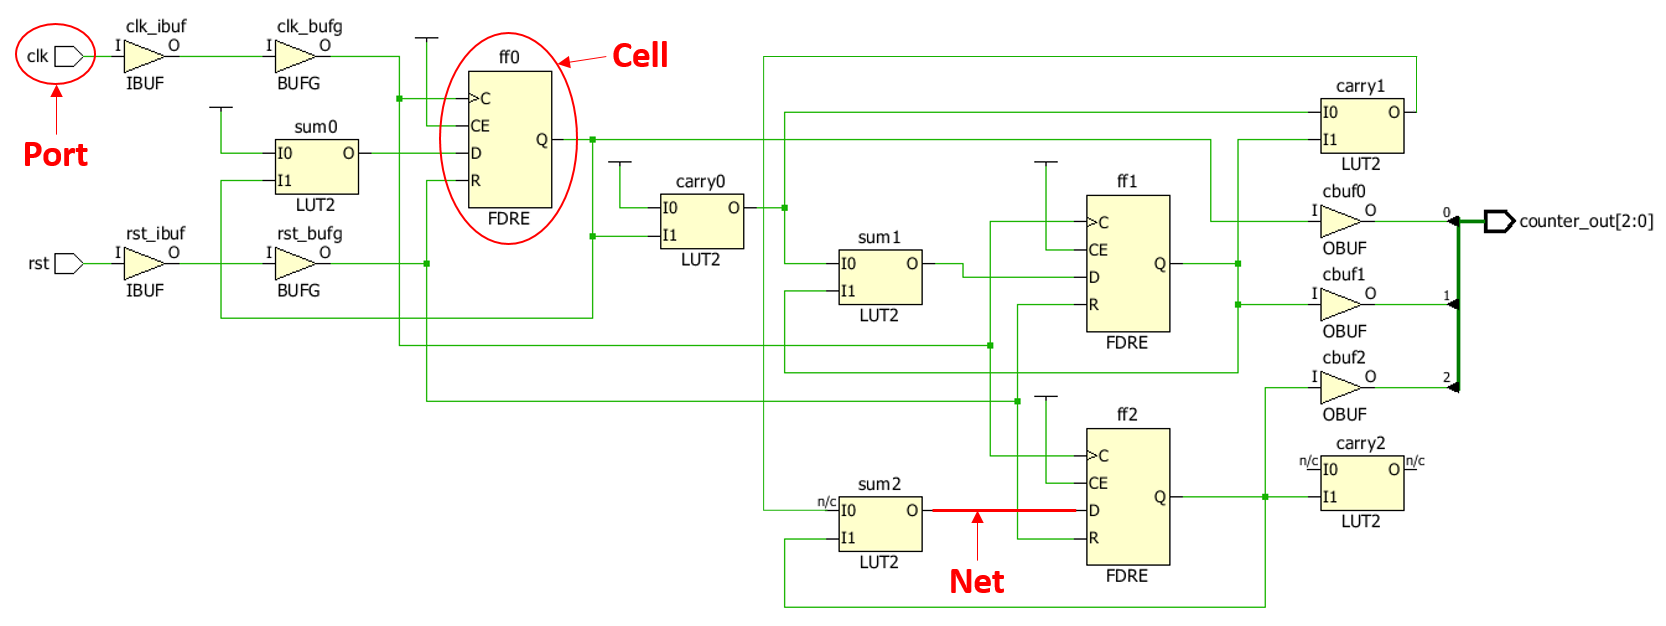
\includegraphics[width=1\columnwidth]{schematic.png}
 \caption{Schematic of a 3-bit counter in Vivado using LUT and FDRE cells.
 The yellow boxes are cells, the green lines are nets, and and the
 white figures on the edge of the diagram are ports.}
 \label{fig:schematic}
\end{figure}

As the figure shows, Vivado netlists are composed of three primary components:
\texttt{Cell}s, \texttt{Net}s, and \texttt{Port}s. Cells are \textbf{instances} of
Xilinx primitives. They are the basic building blocks of a Xilinx netlist and
implement the actual logic of a digital design. The most commonly used
cells include:

\begin{itemize}
  \item \textbf{Look Up Tables} (LUTs): Implement logic equations such as
  $O6 = (A1 + A2) \oplus A3$.
  \item \textbf{Flip-Flops} (FDxx): Single-bit storage elements.
  \autoref{fig:schematic} uses a FDRE cell which specifies a rising-edge
  flip-flop with a reset port, but ties the clock enable port high. Other
  types of FDxx cells can be used to include a clock enable port.
  \item \textbf{Block Ram} (BRAMs): On-chip FPGA memory.
  \item \textbf{Digital Signal Processing Units} (DSPs): Perform complex arithmetic
  functions efficiently.
  \item \textbf{Buffers} (BUF): IO, clock, and other types of signal buffers. 
\end{itemize}

\noindent
Several other types of cells can be used, but the ones in the list above
are the most common. Nets connect cells together. In
other words, the output of one cell is wired to the input of another
cell using a net. Ports are simply design input/output (IO). In terms of a FPGA
design, ports are mapped to specific peripheral pins of the FPGA
for chip IO. It is important to note that a Xilinx netlist is purely logical.
There is no physical information within the netlist (i.e. there is no information about
where the cells have been placed, or how the nets have been routed). When
exporting a design from Vivado, the Xilinx netlist representation is converted
to an electronic design interchange format (EDIF).

%%%%%%%%%%%%%%%%%%%%%%%%%%%%%%%%%%%%%%%%%%%%%%%%%%%
% RapidSmith2 Netlist Data Structures
%%%%%%%%%%%%%%%%%%%%%%%%%%%%%%%%%%%%%%%%%%%%%%%%%%%
\subsection {RapidSmith2 Netlist Data Structures} \label{sec:designDS}
RapidSmith2 netlists are modeled closely after Xilinx netlists. In fact,
much of the terminology between the two are identical or very similar. For those
that are familiar with Vivado designs, this should make the transition to
RapidSmith2 straightforward. The data structures that constitute a RapidSmith2
netlist can be found in the package
\textit{byu.edu.ece.rapidSmith.design.subsite}.
The package hierarchy is shown in \autoref{fig:designDS}.

\begin{figure}[H]
 \centering
 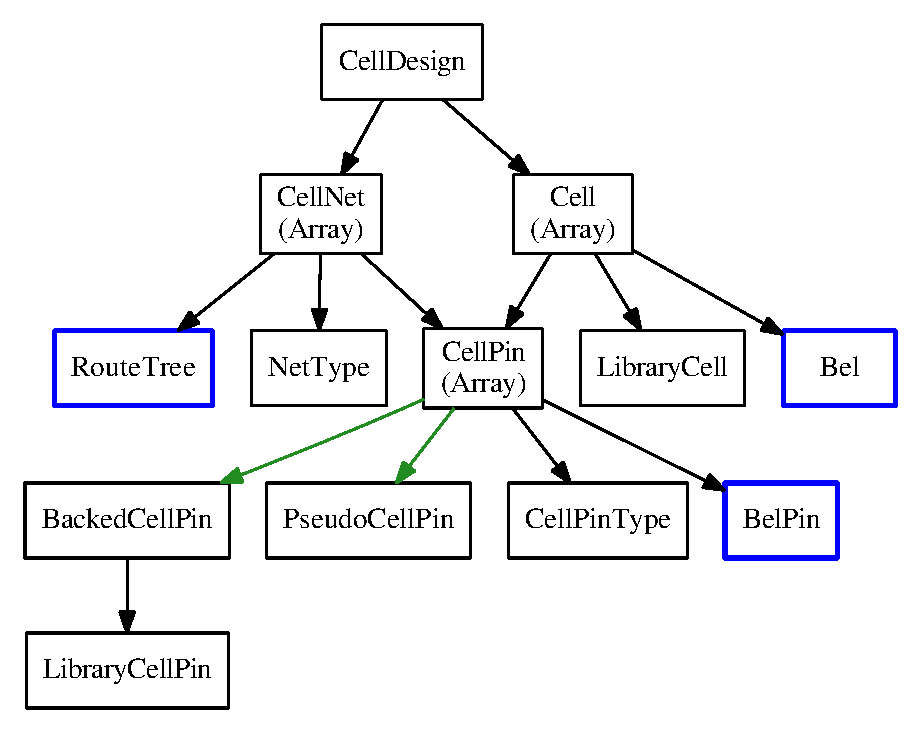
\includegraphics[width=.6\columnwidth]{designDS.eps}
 \caption{RapidSmith2 design data structure tree. Black arrows represent
 composition, green arrows represent inheritance, and blue boxes are physical
 implementation components of the netlist.}
 \label{fig:designDS}
\end{figure}

As can be seen, a \texttt{CellDesign} is the top-level design object in
RapidSmith2. It consists of a collection of \texttt{Cell} objects,
interconnected by \texttt{CellNet}s. RapidSmith2 \texttt{Cell}s are equivalent
to Xilinx cells and RapidSmith2 \texttt{CellNet}s are equivalent to Xilinx nets.
Each \texttt{Cell} has a template \texttt{LibraryCell}, which represents
a Xilinx library primitive (i.e. a LUT). They also have a collection of
connected \texttt{CellPin} objects. Placing and routing these logical design
elements is described in \autoref{sec:placement} and \ref{sec:routing}
respectively. The best way to learn how to utilize the classes shown in
\autoref{fig:designDS} is to generate and read through the
JavaDocs, but important aspects of each class is included in the
following subsections.


\subsubsection{CellDesign} \label{sec:cellDesignDS}
As previously mentioned, the \texttt{CellDesign} class is the top-level netlist
object in RapidSmith2. An instance of a \texttt{CellDesign} contains the
following:

\begin{itemize}
  \item A list of cells
  \item A list of nets 
  \item Global GND and VCC nets
  \item Cell placement information (i.e. where each cell is placed)
  \item The used site PIPs of each site
  \item A list of XDC constraints imported from Vivado. See \autoref{sec:import}
  for more information about XDC constraints and how they are represented in
  RapidSmith2.
  \item The design mode. Possible options include OUT\_OF\_CONTEXT and REGULAR.
  OUT\_OF\_CONTEXT designs are those that have been implemented in Vivado
  ``out-of-context'', meaning that the top-level ports are not placed or routed.
  Most designs are implemented in REGULAR mode.
\end{itemize}

\noindent
The \texttt{CellDesign} class has a variety of methods to retrieve and manipulate
the cells and nets of a design, place cells onto physical BELs, configure
sub-site routing, and perform several other tasks.
 
\subsubsection{Cell}
\texttt{Cell} objects are the building blocks of RapidSmith2 netlists. This
section details some important aspects of \texttt{Cell}s.

\begin {itemize}
  \item A \texttt{Cell} always contains a reference to a backing
  \texttt{LibraryCell} object. A \texttt{LibraryCell} is equivalent to a Xilinx
  primitive cell (described in \autoref{sec:xilinxNetlist}), and serves as a
  template for instantiated \texttt{Cell} objects. The template is used to save
  memory when creating several \texttt{Cell}s of the same type. Whenever a new
  \texttt{Cell} object is created, a corresponding \texttt{LibraryCell} must be
  specified in the constructor. \autoref{code:cells} demonstrates how to create
  new cells in RapidSmith2 and filter cells based on their type.
\end {itemize}  

\begin{lstlisting}[xleftmargin=1.5em, framexleftmargin=1.5em, caption=How to
create new cells in RapidSmith2, label=code:cells] 
// You need to have a cell library to create a cell
CellLibrary libCells = new CellLibrary(RSEnvironment.defaultEnv()
				.getPartFolderPath("xc7a100t-csg324")
				.resolve("cell_library.xml"));

// How to create a new cell. The first argument is the name of the cell, the
// second argument is the library cell
Cell cell = new Cell("myCell", libCells.get("LUT6"));

// Get all cells in a design of a certain type
CellDesign design = getCellDesign();
Stream<Cell> cells = design.getCellsOfType(libCells.get("FDRE"));
\end{lstlisting}

\begin {itemize}
  \item The method call \texttt{CellDesign::getCellsOfType(String,CellLibrary)}
  can be used to get all cells in the current design with a specific type.
  
  \item The methods \texttt{Cell::getPins()},
  \texttt{Cell::getInputPins()}, and \texttt{Cell::getOutputPins()} can be used
  to get a handle to the pins of a \texttt{Cell}. If more pins are
  needed on a \texttt{Cell}, \texttt{PseudoCellPin} objects can be attached (see
  \autoref{sec:pseudoCellPin}). 
  
  \item \texttt{Cell}s can be placed onto \texttt{Bel} objects of the
  current \texttt{Device}. See \autoref{sec:placement} for more information about
  cell placement.
  
  \item Top-level \texttt{Port}s in Vivado (design input/output) are represented as
  Port \texttt{Cell}s in RapidSmith2. Specifically, there are three types of
  port cells: IPORT, OPORT, and IOPORT. The method \texttt{CellDesign::getPorts()} can
  be used to iterate through the ports in a design, and 
  \texttt{Cell::isPort()} can be used to determine if a given \texttt{Cell} is
  actually a port.
  
  \item RapidSmith2 supports both Xilinx macro and leaf cells. More information
  about these is given in \autoref{sec:xilinxNetlist}.
\end{itemize}

\subsubsection{CellPin} \label{sec:cellPin}

\texttt{CellPin}s in RapidSmith2 are attached to \texttt{Cell} objects
and are equivalent to the cell pins found in Vivado. Each \texttt{CellPin}
has an associated \texttt{CellPinType} and \texttt{PinDirection}.
\autoref{tab:pinEnums} displays the possible values for both of these
properties. The \texttt{CellPinType} can be used to find all \texttt{RESET}
pins in a design, determine if a net is a clock net (it connects to pins of type
\texttt{CLOCK}), and help with other useful functions. Cell pins of type
\texttt{PSEUDO} are a special case, and described in \autoref{sec:pseudoCellPin}.
The \texttt{PinDirection} field is typically used to filter a list of
pins on a cell by their direction. It is especially useful for finding INOUT
pins.

\begin{table} [t!]
\caption{Cell Pin Types and Directions}
\begin{center}
\begin{tabu}{ |c|l| }
\hline
\textbf{Property} & \multicolumn{1}{|c|}{\textbf{Values}}\\
\hline
\hline
 & CLEAR \\ 
 & CLOCK  \\
 & ENABLE \\      
 & PRESET \\ 
 & RESET \\
\texttt{CellPinType} & REUSED \\
 & SET \\
 & SETRESET \\
 & WRITE\_ENABLE \\
 & DATA \\
 & PSEUDO \\
\hline
 & IN \\
\texttt{PinDirection} & OUT \\ 
 & INOUT\\ 
\hline
\end{tabu}
\label{tab:pinEnums}
\end{center}
\end{table}

\subsubsection{CellNet}
\texttt{CellNet}s are used to wire components of a logical netlist
together. Specifically, a \texttt{CellNet} connects an output \texttt{CellPin}
to several input \texttt{CellPin}s with the purpose of transferring a signal
from one \texttt{Cell} to another. \autoref{lst:cellNet} shows the basic usage
of \texttt{CellNet} objects in RapidSmith2, and the remainder of this section
details other important aspects about \texttt{CellNet}s.

\newpage
\begin{lstlisting}[xleftmargin=1.5em, framexleftmargin=1.5em, caption=Basic
CellNet functions, label=lst:cellNet] 
  // get a handle to a design
  CellDesign design = getCellDesign();
	
  // creating a new net
  CellNet net = new CellNet("myNet", NetType.Wire);
  design.addNet(net); 
	
  Cell cell1 = design.getCell("cell1");
  Cell cell2 = design.getCell"cell2");
	
  // connecting nets to cell pins
  net.connectToPin(cell1.getSourcePin());
  net.connectToPin(cell2.getpin("a"));
\end{lstlisting}

\begin{itemize}
  \item \texttt{CellNet}s are routed using \texttt{RouteTree} data structures.
  RapidSmith2 routing is described in more detail in \autoref{sec:routing}.
  
  \item All \texttt{CellNet}s have a \texttt{NetType} enumeration. Possible values for
  \texttt{NetType} include VCC, GND, and WIRE. VCC is reserved for power nets, GND
  is reserved for ground nets, and WIRE represents all other nets in the design.
  
  \begin{figure}[t!]
   \centering
   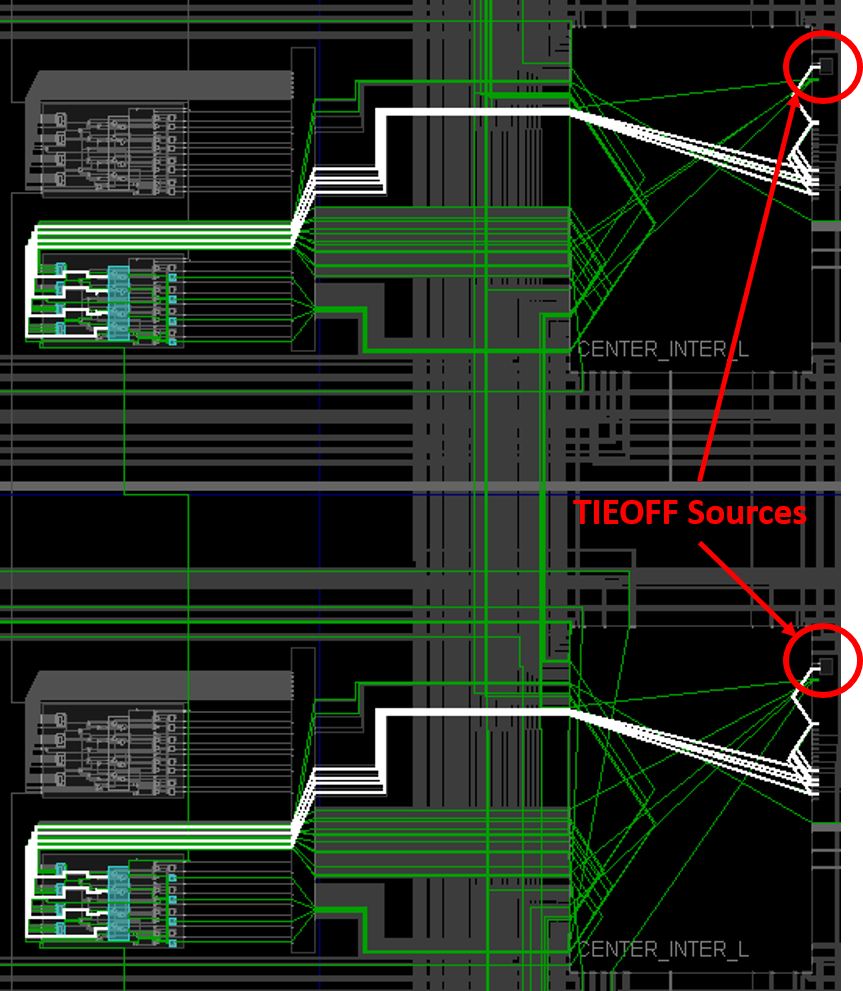
\includegraphics[width=.49\columnwidth]{staticNetSources.png}
   \caption{Example of a Vivado net with multiple sources. The highlighted
   wires in white are all part of the same net.}
   \label{fig:staticNetSources}
  \end{figure}
  
  \item The suggested approach to working with static nets in RapidSmith2 is to
  have only one VCC and GND net in a \texttt{CellDesign}. In general, this
  representation is much easier to work with and the special nets
  can be obtained with the functions \texttt{CellDesign::getVccNet()}
  and \texttt{CellDesign::getGndNet()}. When a design is imported from Vivado
  through a RSCP, all VCC and GND nets are collapsed automatically. Having
  multiple VCC and GND nets, however, is still supported if desired.
  
  \item Most nets have a single driver, but some can be sourced in multiple
  locations. \autoref{fig:staticNetSources} shows an example for a GND
  net. RapidSmith2 handles this oddity by allowing \texttt{CellNet}s to have
  more than one \texttt{RouteTree} object associated with it. In the case of
  \autoref{fig:staticNetSources} the net would have two \texttt{RouteTree}s,
  one for each source TIEOFF.
  
  \item \autoref{fig:iobNet} shows a bidirectional net in Vivado. As can be
  seen, the highlighted net can be driven by both the OBUF output, and from an
  external source via the PAD BEL. RapidSmith2 supports bidirectional nets, 
  and a list of possible drivers can be obtained with the function call
  \texttt{CellNet::getAllSources()}.
  
  \begin{figure}[H]
   \centering
   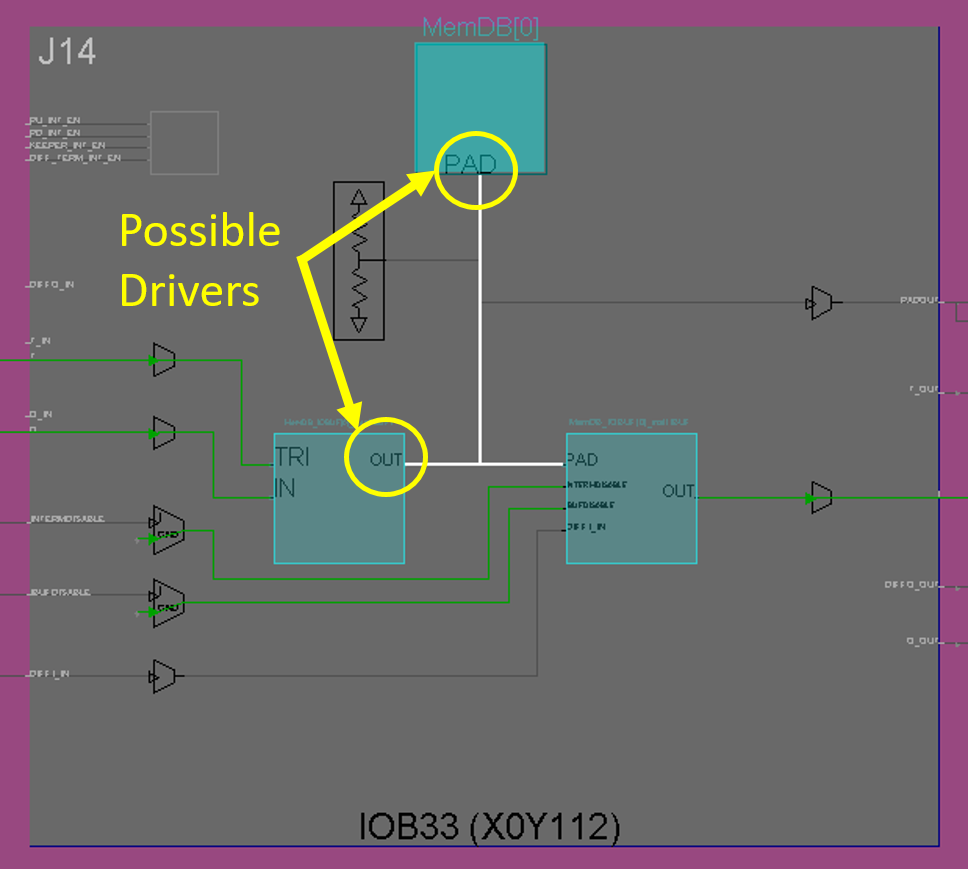
\includegraphics[width=.4\columnwidth]{iobNet.png}
   \caption{Bidirectional Net}
   \label{fig:iobNet}
  \end{figure}

 \begin{figure}[t!]
   \centering
   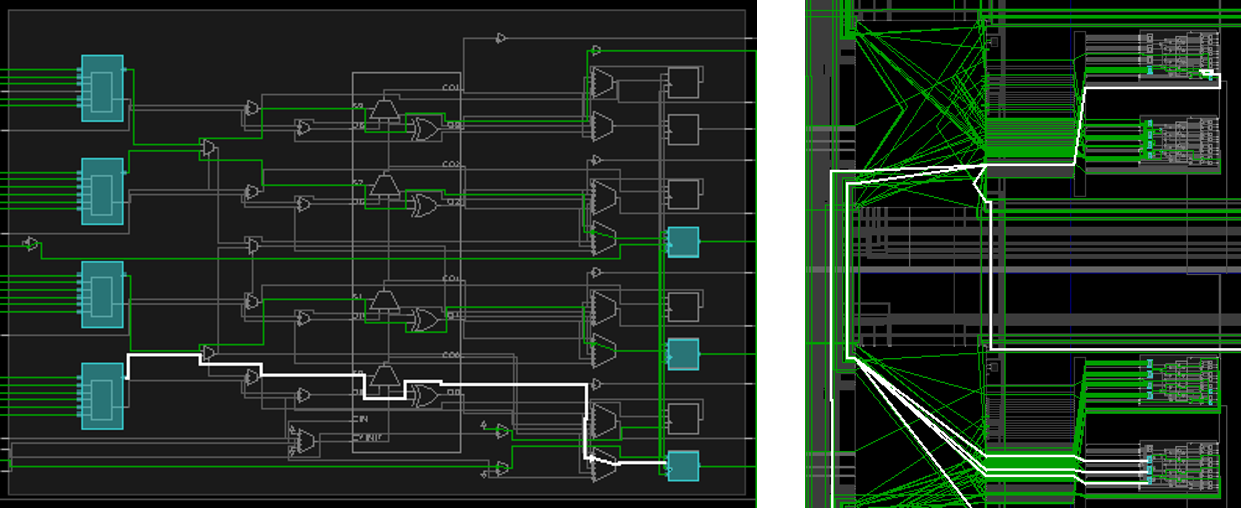
\includegraphics[width=.9\columnwidth]{interVsIntra.png}
   \caption{Example INTRASITE Net (left) and INTERSITE Net (right)}
   \label{fig:interVsIntra}
  \end{figure}
  
  \item After a design has been placed, \texttt{CellNet}s fall into one of two
  categories: \textbf{intrasite} vs. \textbf{intersite}.
  \autoref{fig:interVsIntra} shows an example of both types of nets. As can be
  seen, intrasite nets do not cross site boundaries while intersite nets stretch
  across multiple sites. To determine if a \texttt{CellNet} is an intrasite
  net, the method \texttt{CellNet::isIntrasite()} can be used. 
 
\end{itemize}

\subsubsection{Macro Cells} \label{sec:macros}

Most cells in RapidSmith2 or Vivado designs are leaf cells (LUTs, Flip Flops,
etc.), but Xilinx also supports \textbf{macro} primitives. A macro is a
hierarchical cell that groups one or more leaf cells together to perform a
specific function. An example macro is shown in \autoref{fig:macroCell} for an
IOBUF cell. An IOBUF macro cell contains two \textbf{internal} cells: one of
type OBUFT and the other of type IBUF. It also contains one internal net that
connects the two internal cells together. External cell pins of the macro
connect to one or more internal cell pins.

\begin{figure}[H]
  \centering
  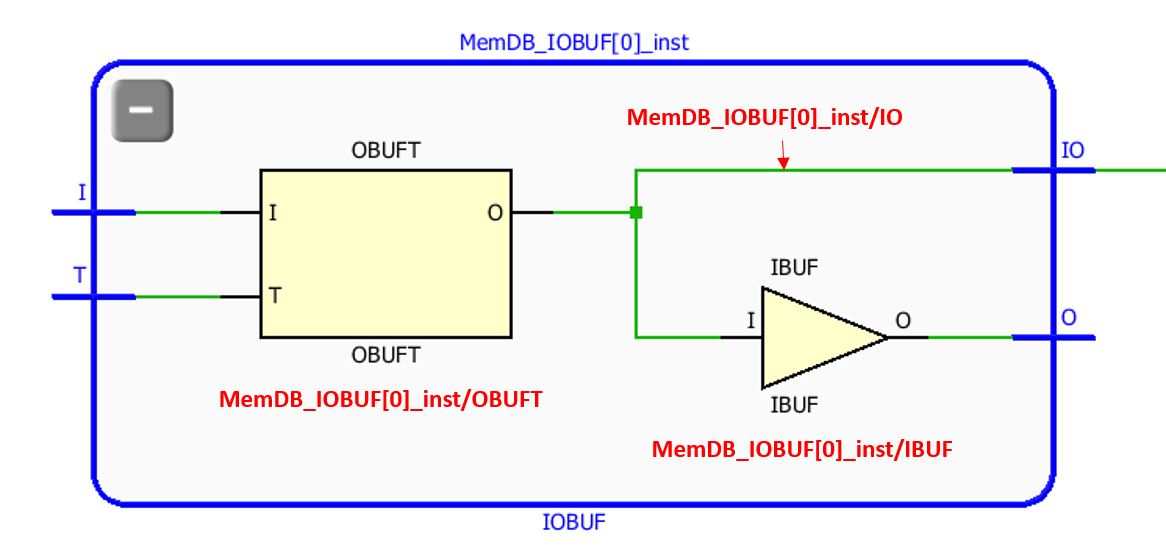
\includegraphics[width=.7\columnwidth]{macroCell.png}
  \caption{Vivado Macro Cell}
  \label{fig:macroCell}
\end{figure}

RapidSmith2 now supports importing macro cells from Vivado and adding them to a
\texttt{CellDesign}. \autoref{code:macros} gives a brief introduction to using
macros in RapidSmith2.

\begin{lstlisting}[xleftmargin=1.5em, framexleftmargin=1.5em, caption=How to use
macros in RapidSmith, label=code:macros] 
// Get a handle to a design and cell library
CellDesign design = getCellDesign();
CellLibrary libCells = getCellLibrary();

// Create a new macro cell and add it to a design
Cell macro = new Cell("myMacro", libCells.get("IOBUF"));
design.addCell(macro);

// Connect the macro cell to a net 
CellPin pin = macro.getPin("IO");
design.getNet("TmpNet").connectToPin(pin);

// Iterate through a list of all cells (macro and leaf cells) of a design
for (Cell cell : design.getCells) {
	if ( cell.isMacro() ) {
		List<Cell> internalCells = cell.getInternalCells();
		List<CellNet> internalNets = cell.getInternalNets();
		List<CellPin> externalPins = cell.getPins();
		// do something with the macro info
	}
	else {
		// do something with a regular leaf cell 
	}
}

\end{lstlisting}

\noindent
As the code example above shows, macro cells are generally used
exactly like regular leaf cells. However, there are a few distinctions
between macro cells and leaf cells.

\begin{itemize}
  \item When a macro cell is added to a design, all internal
  cells and nets are automatically added to the design as well. Users do
  not have to worry about adding these themselves. Similarly, when a macro cell
  is removed from a design, the internal cells and nets are also removed.
  
  \item When a macro cell pin is connected to a \texttt{CellNet}, RapidSmith2
  automatically connects the net to the corresponding internal pins. When a
  macro cell pin is disconnected from a \texttt{CellNet}, the internal cell pins are
  disconnected. Nets in RapidSmith2 only connect to leaf cell pins (i.e. it is
  essentially a flattened netlist with macros cell ``wrappers'').
  
  \item Internal cells and nets within a macro cannot be individually added or
  removed from a design. If this is attempted, an exception will be
  thrown. Instead, the entire macro cell must be added or removed.
  
  \item Macros cannot be placed. Rather, the internal cells of a macro should be
  placed instead.
  
  \item When a \texttt{CellDesign} is exported from RapidSmith, macro cells are not
  exported. The design is first flattened, and only the internal cells and nets
  are exported. This means the macro will not be rebuilt in Vivado, but the
  design will still be functionally equivalent.
\end{itemize}

\subsubsection {PropertyList}

\begin{figure}[b!]
 \centering
 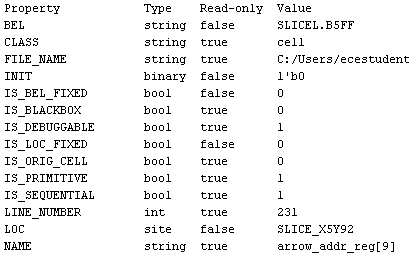
\includegraphics[width=.5\columnwidth]{vivadoProperties.png}
 \caption{Properties of a Vivado FDCE Cell}
 \label{fig:properties}
\end{figure}


Most objects in Vivado's Tcl interface have attached properties. These
properties can be used to describe attributes of the object (such as name,
type, etc.), but they can also be used for configuring the object.
\autoref{fig:properties} shows a list of properties for a FDCE flip flop
cell in Vivado. The Tcl command \texttt{[report\_property \$object]} can be used to
list all properties for a given Vivado object (cell, BEL, etc.). Cells
are the most interesting objects in terms of properties because the function
of a \texttt{Cell} is determined by how it is configured. For example, the
memory width of a BRAM cell in Vivado is configured by setting the
\texttt{READ\_WIDTH} and \texttt{WRITE\_WIDTH} properties of the cell. Possible
values include 1, 2, 4, 9, 18, 36 and 72. The operation of the BRAM is different
depending on how this property is set. Another example is a D flip flop cell
(FDRE) and its \texttt{IS\_C\_INVERTED} property. This property indicates if
the flip flop will be rising-edge or falling-edge triggered. The properties of
cells, nets, and the top-level design are included in the output EDIF netlist
of a RSCP for non-default values only.

When RapidSmith2 parses the EDIF file of a RSCP, the properties
within are stored in a data structure called a \texttt{PropertyList}. Each
\texttt{CellDesign}, \texttt{Cell}, and \texttt{CellNet} in RapidSmith has an
associated \texttt{PropertyList} object. The \texttt{PropertyList} for each
cell in the design also has a list of default configuration properties.
Configuration properties for cells are always included in the
\texttt{PropertyList} even if they are not explicitly set by the user because
the functionality of the cell is dependent on how it is configured.
\autoref{code:properties} shows some basic property usage.

\begin{lstlisting}[xleftmargin=1.5em, framexleftmargin=1.5em, caption=Using
PropertyLists in RapidSmith, label=code:properties] 
// Create a new FF cell with default properties
CellLibrary libCells = getCellLibrary();
LibraryCell libCell = libCells.get("FDRE");
Cell cell = new Cell("myCell", libCell);

// Get a handle to the cells properties
PropertyList properties = cell.getProperties();

// Print the configurable properties of the cell 
for(String propName : libCell.getConfigurableProperties()) {
	Property prop = properties.get(propName);
	System.out.println(propName + ":");
	System.out.println("\tDefault -> " + prop.getStringValue());
	System.out.println("\tPossible -> " + libCell.getPossibleValues(propName)); 
}

// Iterating over a PropertyList
for (Property prop : properties) {
	System.out.println(prop.getKey() " -> " + prop.getStringValue());
}

// Change the FF to be falling edge triggered...this will override the default
property properties.update("IS_C_INVERTED", PropertyType.EDIF, "1'b1");


\end{lstlisting}

\noindent Some additional notes about properties are given below. 

\begin{itemize}
  \item In Vivado, the configurable properties on a cell can be determined by
  using the Tcl command \texttt{[report\_prope\-rty [get\_lib\_cells \$cell]]}.
  All properties that start with ``CONFIG'' are configurable properties that
  can be modified.
  
  \item Because EDIF properties only support String, Integer, and Boolean types,
  any properties imported from the EDIF file will be one of these types.
  It seems, however, that Vivado always exports its properties as strings
  \footnote{RapidSmith makes no attempt to parse the Vivado properties into
  their corresponding data structures. All Vivado properties are represented using
  Strings, and it is currently up to the user to parse the properties if they
  need to}.
 
  \item Only properties of type \texttt{PropertyType.EDIF} will be exported from
  RapidSmith2. When using properties, make sure to mark the type of the property
  as EDIF if you want to export the property to Vivado. All other properties
  will be ignored during design export.
    
\end{itemize}

\subsubsection{Xdc Constraints}
In Vivado, XDC constraint files are used to set the target clock frequency of a
design, constrain a top-level port to a specific package pin on the device, or
specify other physical implementation details. A RapidSmith2 \texttt{CellDesign}
represents these constraints with \texttt{XdcConstraint} objects. Currently,
\texttt{XdcConstraint}s only contain two fields: (1) a command name
(such as \textit{set\_property}) and (2) the command arguments (combined into a
single string). It is the responsibility of the user to parse these XDC
constraints if they need to use them in their CAD tool. The function
\texttt{CellDesign::getVivadoConstraints()} returns a list of constraints
currently attached to a design and \texttt{CellDesign::addVivadoConstraint()}
can be used to add new constraints to a design.

\subsection{Vivado Design Considerations / Advanced Topics}
The previous section detailed the most important aspects of a Vivado 
netlist, and how they are represented in RapidSmith2. However, there are some
subtle considerations for Vivado implemented designs that you need to
understand in order to fully utilize RapidSmith2 as a CAD tool. These design
aspects, and how RapidSmith2 chooses to handle them is described in the
following subsections.

\subsubsection{Pseudo Cell Pins} \label{sec:pseudoCellPin}
Most nets in a Vivado design connect to a set of cell pins, and are routed to
the corresponding BEL pins of those cell pins. VCC and GND nets,
however, can route directly to BEL pins that don't have a connecting cell pin.
An example is shown in \autoref{fig:pseudoCellPin}. As the figure shows, VCC is
routed to the \texttt{A6} pin of the \texttt{D6LUT}, but there is no cell pin
mapped to \texttt{A6} (the input pins of the cell placed at the LUT have
been mapped to \texttt{A1} and \texttt{A4}). The fact that VCC connects to the
\texttt{A6} pin of this LUT is not represented in the logical netlist, and is purely an
implementation detail of the design. Lacking this information is particularly
challenging when developing routing algorithms in external tools. How will the
algorithm know to route to VCC/GND BEL pins when they are not explicitly
represented in the netlist?

\begin{figure}[h!]
  \centering
  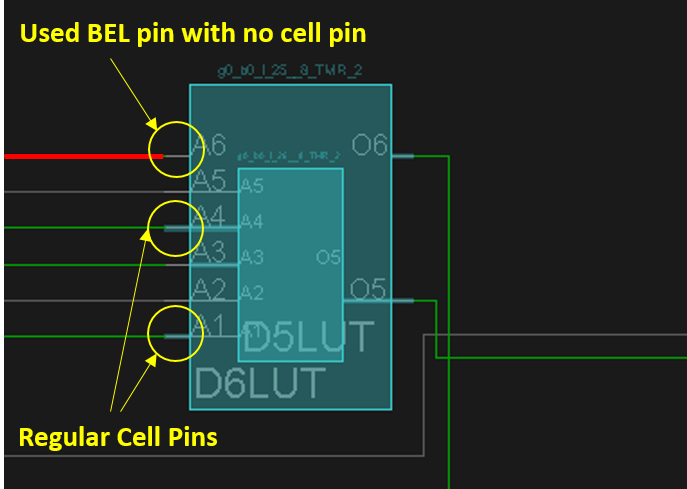
\includegraphics[width=.6\columnwidth]{pseudoCellPin.png}
  \caption{An example of VCC routing to an unused BEL pin (A6)}
  \label{fig:pseudoCellPin}
\end{figure}

To address this issue, RapidSmith2 allows users to create and attach
\texttt{PseudoCellPin}s to an existing cell. A \texttt{PseudoCellPin} is a
``fake'' cell pin that can be attached to a cell (after the cell has been
created), and then attached to a net to create a more complete view of the 
netlist. For example, a \texttt{PseudoCellPin} can be attached to the cell shown
in \autoref{fig:pseudoCellPin}, attached to the VCC net of the design, and then
mapped to the \texttt{A6} pin. Assuming the cell in the figure has the name of
``foo'', \autoref{lst:pseudoPin} demonstrates how to create and attach a new
\texttt{PseudoCellPin}.

\begin{lstlisting}[xleftmargin=1.5em, framexleftmargin=1.5em, caption=Required
function calls to attach a PseudoPin to a Cell, label=lst:pseudoPin] 
  // get a handle to a device and design
  CellDesign design = loadDesign();
  Device device = loadDevice();
  
  // get a handle to the appropriate cells, nets, and bel pins
  Cell cell = design.getCell("foo");
  CellNet vcc = design.getVccNet();
  BelPin bp = device.getSite("SLICE_X0Y179").getBel("D6LUT").getBelPin("A6");
  
  // create and attach the psuedo cell pin, and map it to the BelPin
  CellPin pseudo = cell.attachPseudoPin("VccTmpPin");
  vcc.connectToPin(pseudo);
  pseudo.mapToBelPin(bp);
\end{lstlisting}

\subsubsection {LUT Routethroughs} \label{sec:belRoutethroughs}
Besides their use in implementing logic equations, LUT BELs can also be
configured as PIPs in a fully-routed FPGA design (known as a routethrough). A
LUT is marked as a routethrough when its configuration equation,
\texttt{CONFIG.EQN}, maps the value of a single input pin directly to the
output pin. For timing, the A6 pin is the most preferable option for
a routethrough since it is the fastest, but pins A1-A5 can also be
used in cases of routing congestion. Routethrough LUTs are not explicitly
represented in a design netlist since there is no cell placed on the
corresponding BEL. Figure \ref{fig:routethroughs} shows two example routethrough
LUTs in Vivado. As described in \autoref{sec:routing}, routethroughs are
represented in RapidSmith2 with specific \texttt{Connection} objects, and can be
used when routing a net.

\begin{figure}[h]
  \centering
  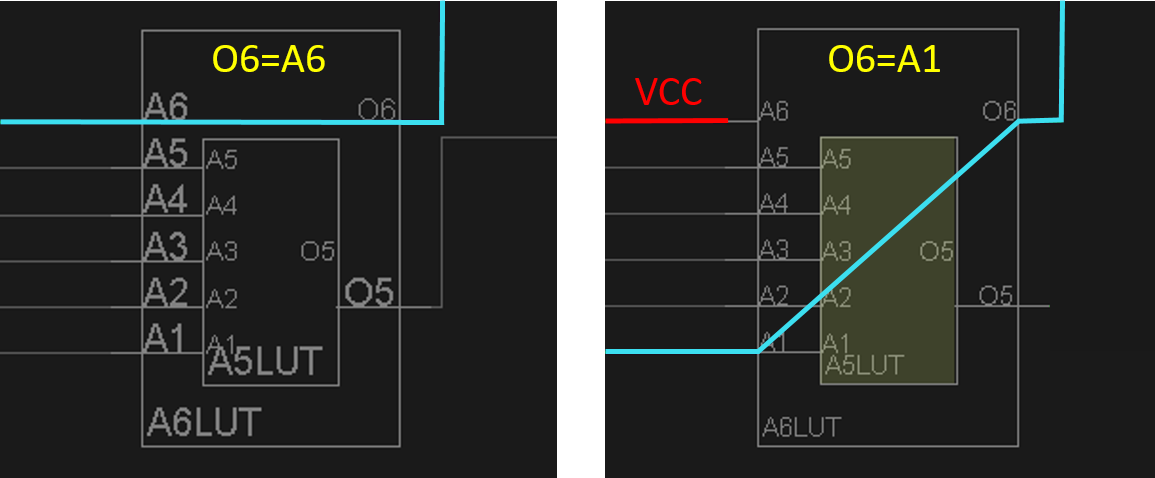
\includegraphics[width=5in]{routethroughs2.png}
  \caption{Two examples of LUTs configured as routethroughs in Vivado. The net
  highlighted in red represents VCC.}
  \label{fig:routethroughs}
\end{figure}

\subsubsection {Permanent Latches}

\begin{figure}[b!]
  \centering
  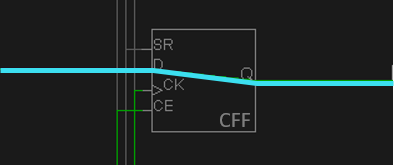
\includegraphics[width=.5\columnwidth]{ffRoutethrough.png}
  \caption{Flip-Flop BEL Configured as a Permanent Latch in Vivado}
  \label{fig:ffRoutethrough}
\end{figure}

A \textbf{permanent latch} in Vivado is a Flip Flop (FF) BEL which has been
configured as a latch with its ``set'' signal tied to VCC. This means that the
data pin of the latch always passes its value to the output pin of the latch,
and no state is retained. An example is shown in \autoref{fig:ffRoutethrough}.
As the figure shows, permanent latches look very similar to LUT routethroughs
described in the previous section. Because of this similarity, RapidSmith2
treates permanent latches the same as LUT routethroughs.

\subsubsection{Static Source LUTs}
Similar to their use as routethroughs, LUT BELs can also be configured as GND or
VCC signal sources. Examples of both are shown in
\autoref{fig:lutStaticSources}. The LUT on the left of the figure drives a VCC
signal and the LUT on the right drives GND. In both cases, the logical
netlist of a design does not represent the use of these LUTs in any way.
RapidSmith2 does explicitly represent static source LUTs. Like other VCC and GND
sources, they are implied based on where a VCC/GND route begins.

\begin{figure}[h]
  \centering
  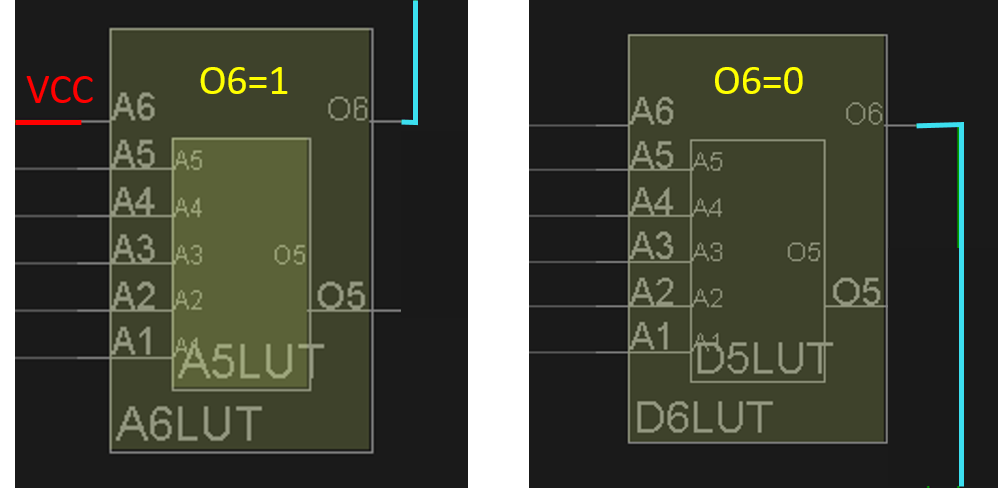
\includegraphics[width=.7\columnwidth]{lutStaticSources.png}
  \caption{Two LUTs Configured as Static Sources in Vivado}
  \label{fig:lutStaticSources}
\end{figure}

\subsubsection{Site PIPs}
\begin{figure}[b!]
  \centering
  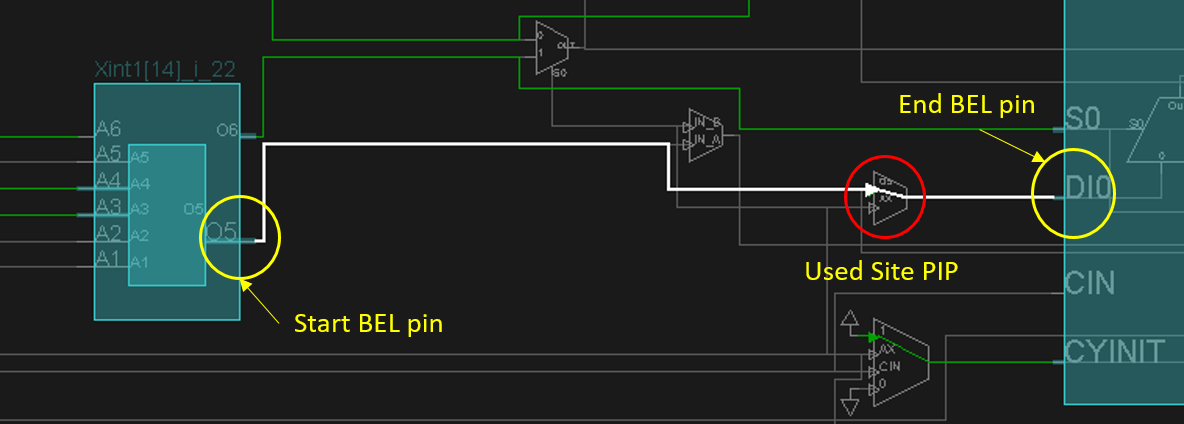
\includegraphics[width=\columnwidth]{sitePips.png}
  \caption{Site PIP Usage}
  \label{fig:sitePips}
\end{figure}

The internal routing structure of nets inside Vivado sites are represented by
a set of used site PIPs. A string of site PIPs enables a connection between site
components. An example is shown in \autoref{fig:sitePips} where the used site
PIPs are circled in red. As can be seen, the \texttt{ACY0:05} site PIP is
enabled and connects the \texttt{05} pin of the \texttt{A5LUT} BEL to the
\texttt{DI0} pin of the \texttt{CARRY4} BEL. Site PIPs can also be used to 
connect site pins to BEL pins. In RapidSmith2, a list of used site PIPs is
stored for each site on design import. The function call
\texttt{CellDesign::getUsedSitePipsAtSite(Site)} can be used to obtain the used
site PIPs at a given site location. After design import, it is the user's
responsibility to update this data structure accordingly.

\subsubsection{Site Properties}
Some properties not only affect how a Cell is configured, but they can also
affect how a Site is configured. For example, on SLICEL sites there exists a
clock routing mux that chooses between a regular clock signal and an inverted
signal (\autoref{fig:clkInv}). The output of this inverter is connected to all
flip flops of the SLICEL, and decides whether \textit{all} flip flops are
rising or falling-edge triggered. The clock that is selected is determined
by the property �IS C INVERTED� \textbf{of the flip flops cells that have been
placed onto the SLICEL}. The clock inverter is programmed automatically based on
the cell properties. There are other such properties, but they will not be listed
here. When creating designs in RapidSmith2, it is important to not place cells
together that may have conflicting properties. RapidSmith2 does not perform any
error checking, and so an error in Vivado will be thrown if you violate
property restrictions.

\begin{figure}[h!]
  \centering
  \includegraphics[width=.8\columnwidth]{clkInv.png}
  \caption{SLICEL clock inverter mux.}
  \label{fig:clkInv}
\end{figure}

%%%%%%%%%%%%%%%%%%%%%%%%%%%%%%%%%%%%%%%%%%%%%%%%%%%
% 	The Cell Library
%%%%%%%%%%%%%%%%%%%%%%%%%%%%%%%%%%%%%%%%%%%%%%%%%%%
\subsection{The Cell Library} \label{sec:cellLibraryinDesignSection}
As described in \autoref{sec:xilinxNetlist}, Xilinx netlists are composed of
cell objects which are instanced from backing library primitives. The most
common library primitives used in a Xilinx netlist include LUT (LUT1,
LUT2, etc) and Flip-Flop (FDRE, FDCE, etc.) cells. A detailed knowledge of the
available library cells for a device is required to perform any useful netlist
modification in external tools. To provide this information, \texttt{Tincr}
defines a \textbf{cell library XML}. A cell library contains the
following information for each library cell that can target a specific device:

\begin {itemize}
  \item Type
  \item Group (i.e. SLICE, DSP, IOB, BRAM, etc.) 
  \item Name, direction, and type for each library cell pin
  \item Valid placement locations for instances of the library cell
  \item Default logical-to-physical pin mappings for each cell pin
  \item Configurable properties with default values
  \item Macro templates 
\end{itemize}

RapidSmith2 parses the cell library XML file described above into a
\texttt{CellLibrary} data structure. This data structure is very useful when
performing any type of netlist manipulation or addition. Currently, each \texttt{CellLibrary}
corresponds to a specific Xilinx part. This means that for each device file in
RapidSmith2, a new \texttt{CellLibrary} needs to be generated \footnote{This may
change to be family-specific in the future, but usually, parts in the same
family can use the same \texttt{CellLibrary}.}. \autoref{code:cellLibrary}
shows two ways to load a \texttt{CellLibrary} in RapidSmith2. The following
subsections detail important aspects of a cell library.

\begin{lstlisting}[xleftmargin=1.5em, framexleftmargin=1.5em, caption=
Loading a CellLibrary in RapidSmith2, label=code:cellLibrary] 
// First way, load a Tincr Checkpoint
VivadoCheckpoint vcp = VivadoInterface.loadRSCP("checkpoint.rscp");
CellLibrary libCells1 = vcp.getLibCells();

// Second way, directly load the cell library from disk
CellLibrary libCells2 = new CellLibrary(RSEnvironment.defaultEnv()
                       .getPartFolderPath("xc7a100t-csg324-3")
                       .resolve("cellLibrary.xml");
\end{lstlisting} 

\subsubsection{Generating A New Cell Library} \label{sec:cellLibraryGeneration}
The \texttt{Tincr} command \texttt{[tincr::create\_xml\_cell\_library]} can be
used to generate a new cell library for a device. Specifically, follow the steps
listed below to create a new cell library (the items marked with
\textbf{SERIES7} only need to be done for series7 families).

\begin{enumerate}
  \item Open Vivado in Tcl mode, and run the command shown in the listing below.
  Replace ``xc7a100tcsg324-3'' with the part you want to generate and
  ``mycellLibrary.xml'' with the location where you want to store the generated
  cell library XML. This will generate most of what you need in the cell
  library XML automatically.
\end{enumerate}

  \begin{lstlisting} [numbers=none,keywordstyle=\ttfamily]
  Vivado% ::tincr::create_xml_cell_library xc7a100tcsg324-3 mycellLibrary.xml
  \end{lstlisting}

\begin{enumerate}
 \setcounter{enumi}{1} 
  \item \textbf{SERIES7}: Open the generated XML file in a text editor and
  search for the ``CARRY4'' cell. Scroll down to the ``bels'' XML element within
  the CARRY4 cell, and add the following lines to each pin that is named ``CI'':
  
  \begin{figure}[H]
   \centering
   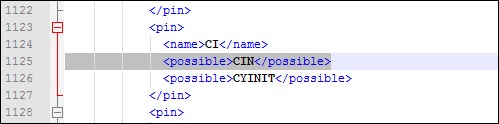
\includegraphics[width=.9\columnwidth]{cellLibHandEdit.png}
  \end{figure}
  
  You should have to insert this line in two places only.
  \item \textbf{SERIES7}: Save your changes and exit the text editor
  \item Copy the XML file to \textit{RapidSmithPath/device/family}
  directory where ``family'' is replaced by the family of your part (such as
  artix7), and ``RapidSmithPath'' is the location of your RapidSmith repository.
  Once this is complete the new \cls{CellLibrary} should be ready to use. 
\end{enumerate}

\subsubsection{Adding Custom Macros to a Cell Library} \label{sec:customMacros}
Customized, user-defined macros can be added to a RapidSmith2 \cls{CellLibrary}
if desired. This can be accomplished in two easy steps. 

\begin {enumerate}
  \item Create an XML specification
  of your macro that follows the format laid out below: 
\end {enumerate}

\begin{lstlisting}[language=XML, numbers=none, keywordstyle=, stringstyle=,
label=lst:macroXml, caption=Sample Macro XML for a CellLibrary] 
<?xml version="1.0" encoding="UTF-8"?> <root>	
  <macros>    
		<macro>
        <type>RAM128X1D</type>
        <!-- List of internal cells with name and leaf type of each -->
        <cells>
            <internal>
                <name>DP.HIGH</name>
                <type>RAMD64E</type>
            </internal>
            <internal>
                <name>DP.LOW</name>
                <type>RAMD64E</type>
            </internal>
            <internal>
                <name>F7.DP</name>
                <type>MUXF7</type>
            </internal>
			...
        </cells>
        <!-- List of macro pins with name, direction, pin type, and internal connections --> 
        <pins>
            <pin>
                <name>DPO</name>
                <direction>output</direction>
                <type>MACRO</type>
                <internalConnections>
                    <pinname>F7.DP/O</pinname>
                </internalConnections>
            </pin>
            <pin>
                <name>SPO</name>
                <direction>output</direction>
                <type>MACRO</type>
                <internalConnections>
                    <pinname>F7.SP/O</pinname>
                </internalConnections>
            </pin>
            <pin>
                <name>A[6]</name>
                <direction>input</direction>
                <type>MACRO</type>
                <internalConnections>
                    <pinname>F7.SP/S</pinname>
                    <pinname>DP.HIGH/WADR6</pinname>
                    <pinname>DP.LOW/WADR6</pinname>
                    <pinname>SP.HIGH/WADR6</pinname>
                    <pinname>SP.LOW/WADR6</pinname>
                </internalConnections>
            </pin>
            ...
        </pins>
        <!-- List of internal nets, and the internal cell pins they connect to --> 
        <internalNets>
            <internalNet>
                <name>DPO0</name>
                <pins>
                    <pinname>F7.DP/I0</pinname>
                    <pinname>DP.LOW/O</pinname>
                </pins>
            </internalNet>
            ...
        </internalNets>
    </macro>
	...
  </macros>
</root>
\end{lstlisting}

\begin{enumerate}
 \setcounter{enumi}{1} 
  \item Import the macro into the \cls{CellLibrary} using the API call shown in
  \autoref{code:macroImport}.

\end{enumerate}

\begin{lstlisting}[caption=Adding new macros to the Cell Library,
label=code:macroImport] 
// Get a handle to a CellLibrary
CellLibrary libCells = getCellLibrary();

// Add the macros in an XML file.
libCells.loadMacroXML(Paths.get("myMacro.xml"); 
\end{lstlisting}

\noindent
Once this is complete, you can use your custom macro in a \cls{CellDesign} like
a normal cell.


%%%%%%%%%%%%%%%%%%%%%%%%%%%%%%%%%%%%%%%%%%%%%%%%%%%%%%%%%%%%%%%%%%%%%%%%%%%%%%%%%%%%%%%%%
% Section 6: Placement in RapidSmith2
%	This section contains a description of the following:
%	- How to place cells onto BELs and map cell-pins to bel-pins in RS2
%	- How to get a list of valid placement locations for a cell  
%	- Placement special cases
%%%%%%%%%%%%%%%%%%%%%%%%%%%%%%%%%%%%%%%%%%%%%%%%%%%%%%%%%%%%%%%%%%%%%%%%%%%%%%%%%%%%%%%%%
\newpage
\section{Placement} \label{sec:placement}

In the original RapidSmith, placement occurred at the \cls{Site} level. A
collection of \cls{Cell}s were grouped together in what was called an
\cls{Instance}, and the \cls{Instance} was assigned to a compatible site type.
Where the individual \cls{Cell}s were actually placed within the \cls{Site}
was a blackbox. Because RapidSmith 2 breaks up a \cls{Site} into its
individual components, \cls{Cell}s can now be placed directly onto
physical \cls{BEL}s within a \cls{Site}. This gives Xilinx FPGA CAD developers
finer grain control during the placement of a design, and allows sub-site
algorithms (such as packing algorithms) to be explored. \autoref{code:place}
demonstrates the basic steps to placing a \cls{Cell} in RapidSmith.

\begin{lstlisting} [caption=Steps for placing a Cell in RapidSmith,label=code:place]
// Load the device and design
TincrCheckpoint tcp = VivadoInterface.loadTcp("myCheckpoint.tcp"); 
Device device = tcp.getDevice();
CellDesign design = tcp.getDesign();

// Get a handle to a Cell and Bel. The cell is of type LUT2 
Cell cell = design.getCell("MyCell"); 
Bel bel = device.getSite("SLICE_X40Y137").getBel("D6LUT");

// Place the cell onto the bel
design.placeCell(cell,bel);

// Two ways to map bel pins
CellPin pin1 = cell.getPin("I0");
CellPin pin2 = cell.getPin("I1");
CellPin pin3 = cell.getPin("O")

// First way
pin1.mapToBelPin(bel.getPin("A1"));
pin2.mapToBelPin(bel.getPin("A2"));

// Second way
List<BelPin> possible = pin3.getPossibleBelPins(bel);
pin3.mapToBelPin( possible.get(0) );
\end{lstlisting}

\noindent
As the code listing shows, there are two steps to placing a RapidSmith
\cell. The first is straightforward: get a handle to a \bel object,
and use the method call \texttt{CellDesign.placeCell(Cell, Bel)} (line 11). This
will map a logical \cell onto a physical \bel. Once a \bel has been
used, no other \cells can be mapped to it. No error checking is performed to
ensure that a \cell is compatible with the \bel it is being placed on, that is
up to the user. The second step is more complicated: each logical \cellpin of
the \cell needs to be mapped to a physical \belpin. This can be done by
either (a) specifying the \belpin name (lines 19-20), or (b) using
the function call \texttt{CellPin.getPossibleBelPins(Bel)} (line 23) to
get a list of valid \belpin mappings. For most \cells each \cellpin only
maps to a single \belpin, and so option (b) is preferable. However, there are two
noticable exceptions to this rule.

\begin {enumerate}
  \item LUT input pins are permutable. This means that an input \cellpin 
  attached to a LUT \cell can be mapped to any input pin of a LUT \bel.
  \autoref{fig:lutPins} shows an example of this functionality in Vivado. Once
  the input pins have been mapped, a configuration equation is created for and
  applied to the LUT \bel using the appropriate \belpin inputs.
  In order for a LUT \cell to be physically implemented, these pins need to be
  mapped. The function call \texttt{CellPin.getPossibleBelPins(Bel)} in this
  case will return all of the input \belpins of the LUT and the user can decide
  which ones to use.
  
  \begin{figure}[t]
	\centering
	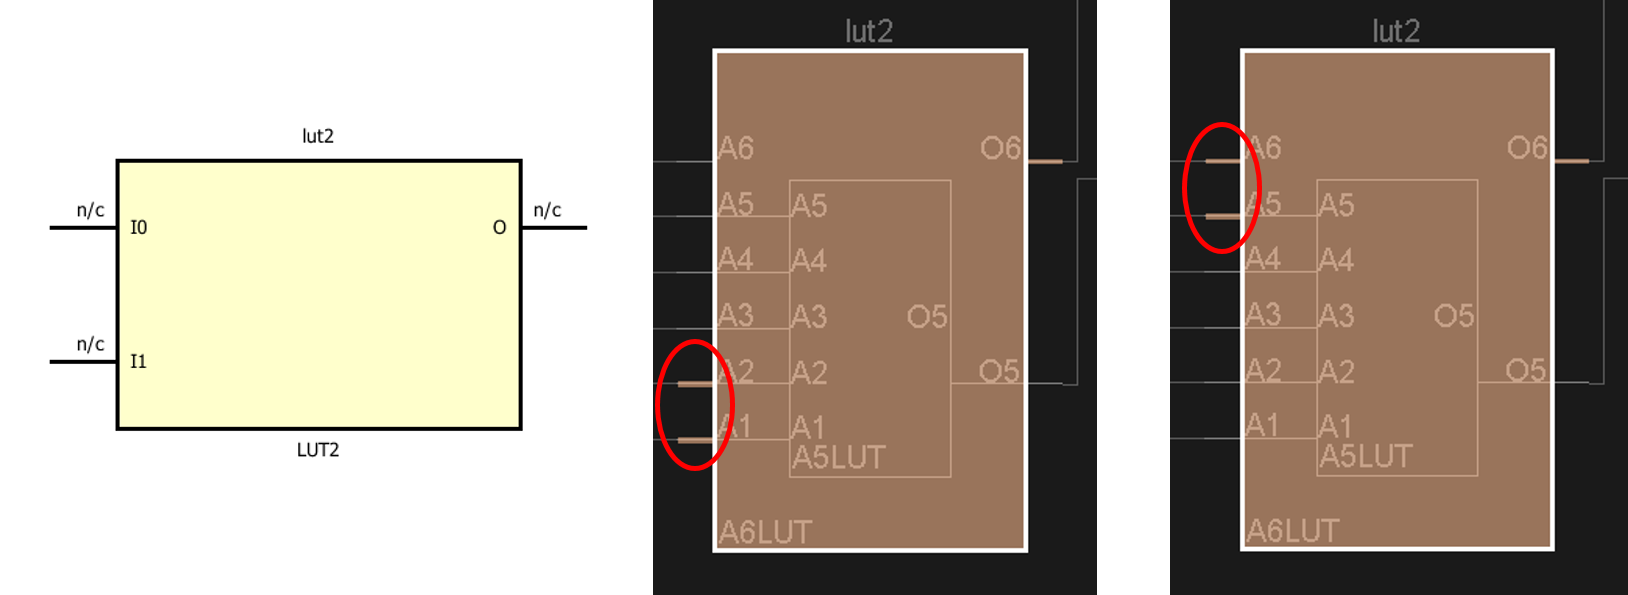
\includegraphics[width=1\columnwidth]{lutPins.png}
	\caption{An example of LUT pin permutations. The left figure shows the
	schematic of a LUT2 cell. The middle figure shows the two input pins of the LUT
	cell being mapped to the A1 and A2 pins of a LUT6 bel. The right figure shows
	the same input pins being mapped to the A6 and A5 pins instead.}
	\label{fig:lutPins}
  \end{figure}
  
  \item Logical-to-physical pin mappings can change \pgm{based on how a cell is
  configured}. For example, on a RAMB36E1 \cell, the least-significant data
  input pins map to different physical \belpins when the width of the BRAM is
  set to 72. This is an important concept when performing netlist modifications
  in RapidSmith. The function call \texttt{CellPin.getPossibleBelPins(Bel)} only
  returns the pin mappings for the \pgm{default} \cell configuration. The
  correct pin mappings are always used when a Tincr checkpoint is imported into
  RapidSmith, but if new logic is being added to a design it is up to the
  user to determine the proper pin mappings. Adding support for
  automatically determining a \cells pin mappings based on a its
  configuration is currently being worked on, but is not yet ready. For now,
  users can configure a cell in Vivado, place it, and use the TCL function shown
  in \autoref{code:tclPinMap} to determine the correct pin mappings for a \cell.

\end{enumerate}

\begin{lstlisting}[language=tcl, caption=TCL script to print all
logical-to-physical pin mappings of a cell,label=code:tclPinMap]

proc print_pin_mappings{cell} {

	foreach cell_pin [get_pins -of $cell] {
		puts "$cell_pin -> [get_bel_pins -of $cell_pin]" 
	}
}

\end{lstlisting}
 
\vspace{.2cm}
\noindent
Some additional points about placement to be aware of include: 

\begin {itemize}
  \item VCC and GND \cells are not placed when implementing a design in Vivado.
  This distinction is applied to RapidSmith 2 as well. Rather than placing VCC
  or GND explictly, \cls{RouteTree}s that are sourced by switchbox TIEOFFs are
  used to express their placement implicitly (VCC/GND is ``placed'' on the
  TIEOFF).
  \item A list of valid placement options for a \cell can be obtained with the
  function call \texttt{Cell.getPossible\-Anchors()}. The sample program
  \pgm{CreateDesignExample} (described in \autoref{sec:createDesignExample})
  gives a good example of how to use this function. The reader is referred to
  the source code and Javadocs for more details.
  \item If you plan on writing a placer in RapidSmith, there are several
  placement rules for a given device. A few examples include (a) CARRY4 \cells
  that are connected through the carry chain need to placed vertically to one
  another so they can use the dedicated carry wires, and (b) A RAMB36E1 cell
  cannot be placed in the same tile as a RAMB18E1 cell. If either of these
  rules are violated, an error will be thrown in Vivado. It is the
  responsibility of the user to determine all relevant placement rules
  because error checking is not performed on design export. The source code for
  a sample simulated annealing placer for the Artix-7 part {\em
  xc7a100tcsg324} can be found in the package
  \pkg{edu.byu.ece.rapidSmith.examples.placerDemo}.
  \item Macro cells in RapidSmith cannot be placed. The internal cells of a
  macro should be placed instead.
\end{itemize}

%%%%%%%%%%%%%%%%%%%%%%%%%%%%%%%%%%%%%%%%%%%%%%%%%%%%%%%%%%%%%%%%%%%%%%%%%%%%%%%%%%%%%%%%%
% Section 7: Routing in RapidSmith2
%	This section contains a description of the following:
%	- Wires and connection types in RapidSmith2 (wire connections, routethroughs, etc.)
%	- How to route nets in RapidSmith2 using RouteTrees
%	- Three-part routing structure for nets.
%	- Vivado ROUTE strings and intrasite routing.
%%%%%%%%%%%%%%%%%%%%%%%%%%%%%%%%%%%%%%%%%%%%%%%%%%%%%%%%%%%%%%%%%%%%%%%%%%%%%%%%%%%%%%%%%
\newpage
\section{Routing} \label{sec:routing}
\graphicspath{{./techReportFigures/sec7_routing/}}

During placement, all cells of a design are mapped to BELs, and all
cell pins are mapped to BEL pins. The next (and final) step of the
FPGA implementation flow is to physically wire together the used BEL pins. This
is known as routing. Routing involves taking each logical net of a design,
determining the BEL pins they are connected to (based on the cell pins), and
finding a list of physical wires that electrically connect the pins together.
This section details how routing algorithms can be implemented in RapidSmith2.

\subsection{Wires and Wire Connections} \label{wireConnSection}
Routing in RapidSmith2 is done using \texttt{Wire} objects, which are described
in subsection \ref{wireSection}. \texttt{Wire}s are uniquely identified by
their corresponding tile and wire name (i.e. ``tileName/wireName''), and are connected
through \texttt{Connec\-tion} objects. There are two types of wire connections:

\begin {enumerate}
  \item \textbf{PIP Connections}: Connect two different wires through a
  Programmable Interconnect Point. Most PIP connections are found in
  switchbox tiles of a FPGA part (as shown in \autoref{fig:switchboxPIP}).
  These types of connections are important to FPGA routing, because they
  dynamically configure the routing network for a given design.
   
  \item \textbf{Non-PIP Connections}: Connect the same physical wire across two
  different tiles. In general, wires stretch across multiple tiles in a device, having
  a different name in each tile. This is demonstrated in
  \autoref{fig:wireFigure}. The example wire shown in the figure spans 5
  tiles, but has a different name in each. To save space, only the
  source and sink wire segments are kept in RapidSmith2 data structures
  (i.e. \texttt{INT\_X1Y1/E2BEG4}, \texttt{INT\_X2Y1/E2MID4}, and
  \texttt{INT\_X3Y1/E2END4}). The source segment is connected to each sink
  segment through a non-PIP wire connection. It is also possible to have non-PIP
  connections within a tile, but this is rare.
\end{enumerate} 

\begin{figure}[h!]
\centering
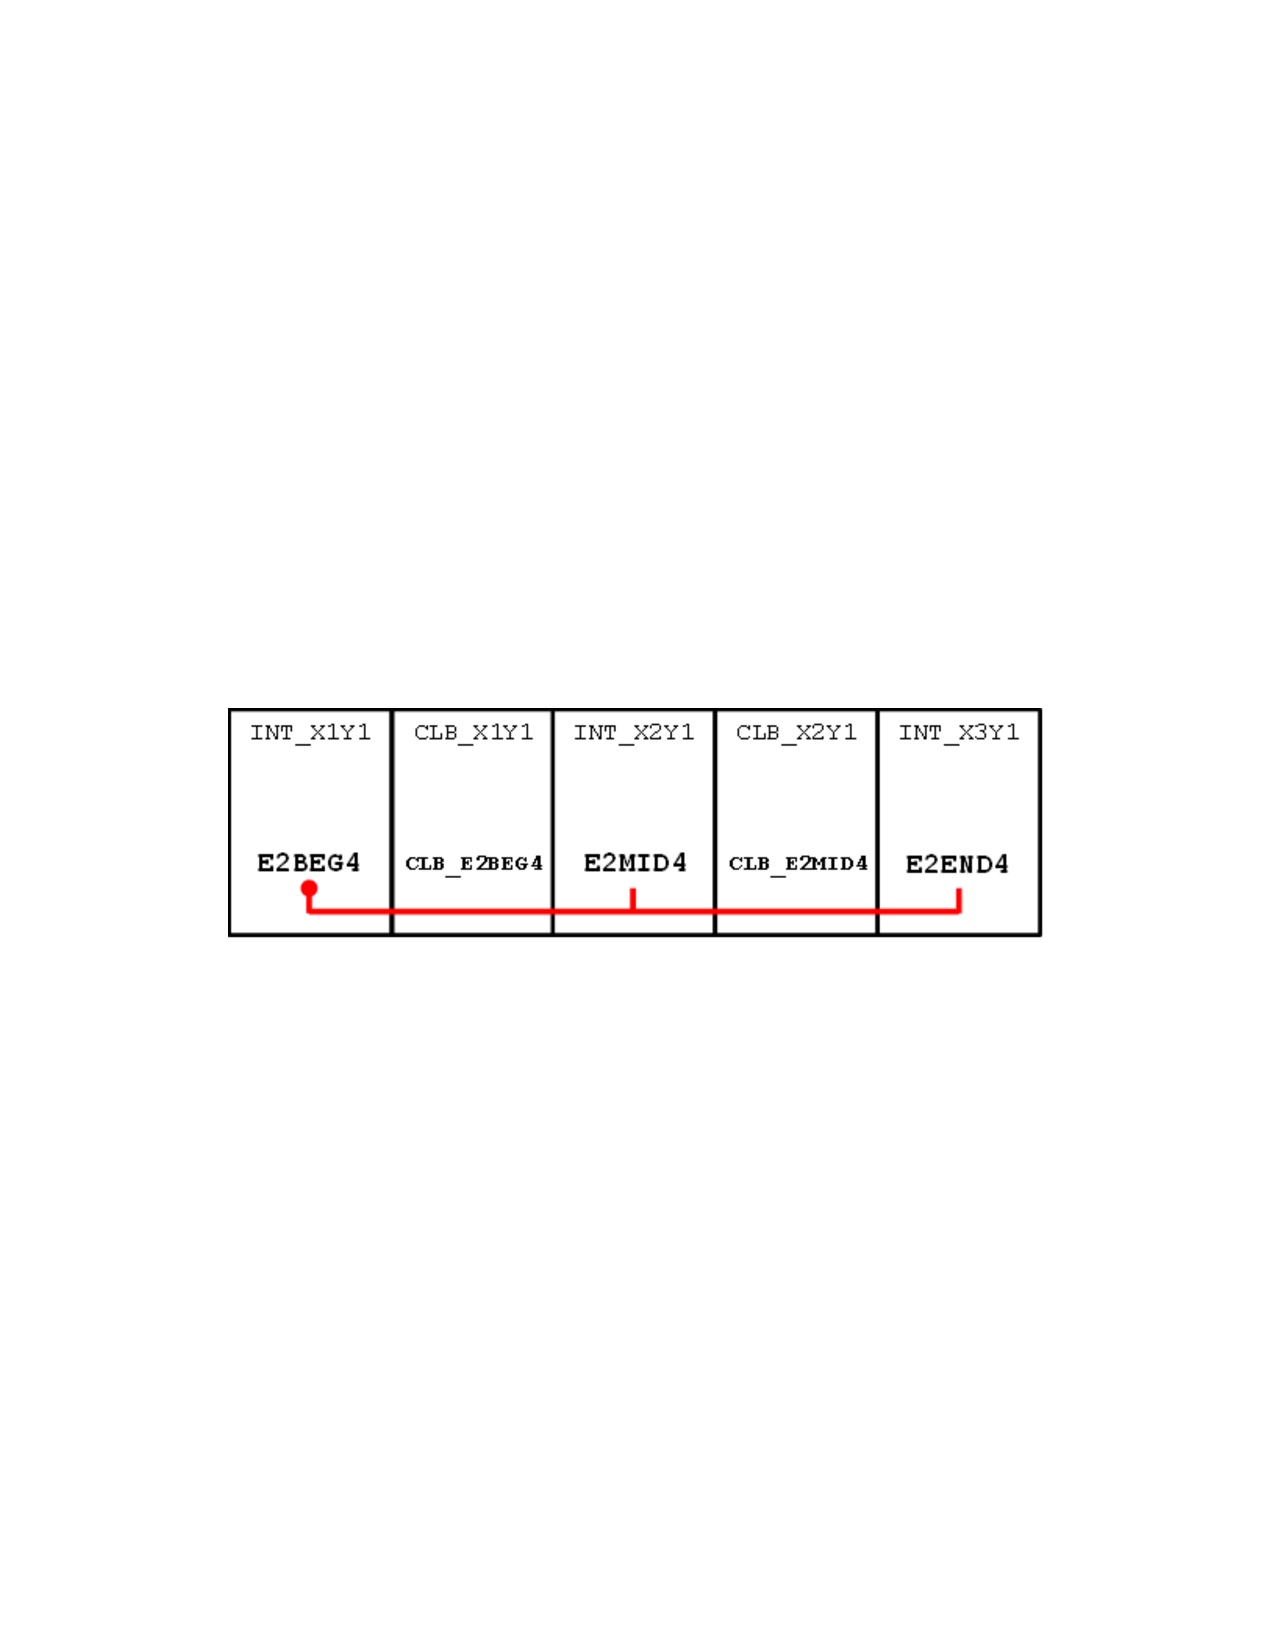
\includegraphics[width=0.8\columnwidth]{wireFigure}
\caption{Multi-Tile Xilinx Wire}
\label{fig:wireFigure}
\end{figure}

\subsection{Traversing Wire Objects}
Traversing through wires in a device is straightforward. Given a handle to a
\texttt{Wire} object named "mywire" or a \texttt{Connection} object named
"conn", the following function calls can be used:

\begin {itemize}
  \item \texttt{mywire.getWireConnections()}: Returns a collection of all
  \texttt{Connection} objects whose source is ``mywire''. This collection can
  be iterated over to find all places a specific wire goes (i.e. what wires it
  connects to).
  \item  \texttt{conn.isPip()}: Returns true if the wire connection ``conn'' is
  a PIP connection. Returns false otherwise.
  \item \texttt{conn.getSinkWire()}: Returns the sink wire of a wire connection.
\end{itemize} 

\noindent
In general, these are the only three functions that are needed to
search through the wires of a FPGA device. It is important to note however that
the first wire in the route must be either (a) created using a \texttt{TileWire}
constructor, or (b) retrieved from a function call of another object (such as
\texttt{SitePin::getExternalWire()}). \autoref{code:connections} demonstrates
how to iterate over \texttt{Connection} objects. To gain a better
understanding of how to use \texttt{Wire}s and \texttt{Connection}s, see the
\textbf{HandRouter} example in the RapidSmith2 repository.

\subsection{Other Types of Connections} \label{otherConns}
Along with PIP and non-PIP wire connections, there are several other types of
connections in RapidSmith2. The source of the connection is always a
\texttt{Wire} object, but the sink object differs. A description of these
connections is found below:

\begin {itemize}
  
  \item \textbf{Site Pin Connections}: Connects a \texttt{Wire} to a
  \texttt{SitePin}. The function call \texttt{Connection::.get\-SitePin()} can
  be used to return a handle to the site pin.
  
  \item \textbf{Terminal Connections}: Connects a \texttt{Wire} to a \texttt{BelPin}. The
  function call \texttt{conn.get\-BelPin()} can be used to return a handle to
  the BEL pin.
  
  \item \textbf{Site Routethrough Connections}: Connects an input site \texttt{Wire}
  to an output site \texttt{Wire}. A \texttt{Site} in Vivado can be configured to pass
  the signal on an input pin directly to an output pin. These connections are
  represented as routethroughs in RapidSmith2 and can be determined with the
  function call \texttt{Connection::isRoutethr\-ough()}.
  \textbf{NOTE}: Before using this type of connection when building a
  routing data structure, make sure the corresponding site is unused.
  
  \item \textbf{BEL Routethrough Connections}: Connects an input BEL \texttt{Wire} to
  an output BEL \texttt{Wire}. LUTs in Vivado can also be configured as
  routethroughs. A BEL routethrough connection can be used while routing the
  inside of a site if there is no cell placed on the
  corresponding BEL.
\end{itemize}

\noindent
When traversing through the device data structure, a generic \texttt{Connection}
object is usually used. This connection can refer to any of the connections
described so far in this documentation. \autoref{code:connections} demonstrates
how to iterate through different \texttt{Connection} types in RapidSmith2.

\begin{lstlisting}[xleftmargin=1.5em, framexleftmargin=1.5em, caption=How to
iterate over Connections in RapidSmith2, label=code:connections] 
  // Get a handle to a wire
  Wire wire = sitePin.getExternalWire();

  // Iterate over all WireConnections
  for (Connection conn : wire.getWireConnections()) {
	  Wire sinkWire = conn.getSinkWire();

	  if (conn.isPip()) {
		  // Do something with a PIP
	  } 
	  else if (conn.isRoutethrough()) {
		  // Do something with a routethrough
	  } 
	  else {	
		  // Do something with a regular wire connection				
	  }
  }

  // Get the site pin connected to a wire
  SitePin pin = wire.getConnectedPin();
  if (pin != null)
	  // Do something with the SitePin
  }

  // Get the bel pin connected to a wire
  BelPin pin = wire.getTerminal();
  if (pin != null)
	  // Do something with the BelPin
  }

  // Iterate over all connections at the same time
  Iterator<Connection> connIt = wire.getAllConnections().iterator();

  while (connIt.hasNext()) {
	  Connection conn = connIt.next();
	
	  if (conn.isPinConnection()) {
		  //do something with the site pin
	  }
	  else if (conn.isTerminal()) {
		  //do something with the bel pin 
	  }
	  else if (conn.isPip()) {
		  //do something with the pip wire connection
	  }
	  else {
		  //do something with regular wire connection.
	  }
  }
\end{lstlisting}

\subsection{RouteTrees}

\texttt{Wire}s and \texttt{WireConnection}s are the fundamental objects used to
specify and explore routing in RapidSmith2, but they need to be organized in
a higher-level data structure to give meaning to the route of a \texttt{CellNet}.
In the original RapidSmith, creating this data structure was up to the user.
RapidSmith2 introduces the \texttt{RouteTree}, which can be seen in
\autoref{fig:routeTreeDS}.

\begin{figure}[H]
\centering
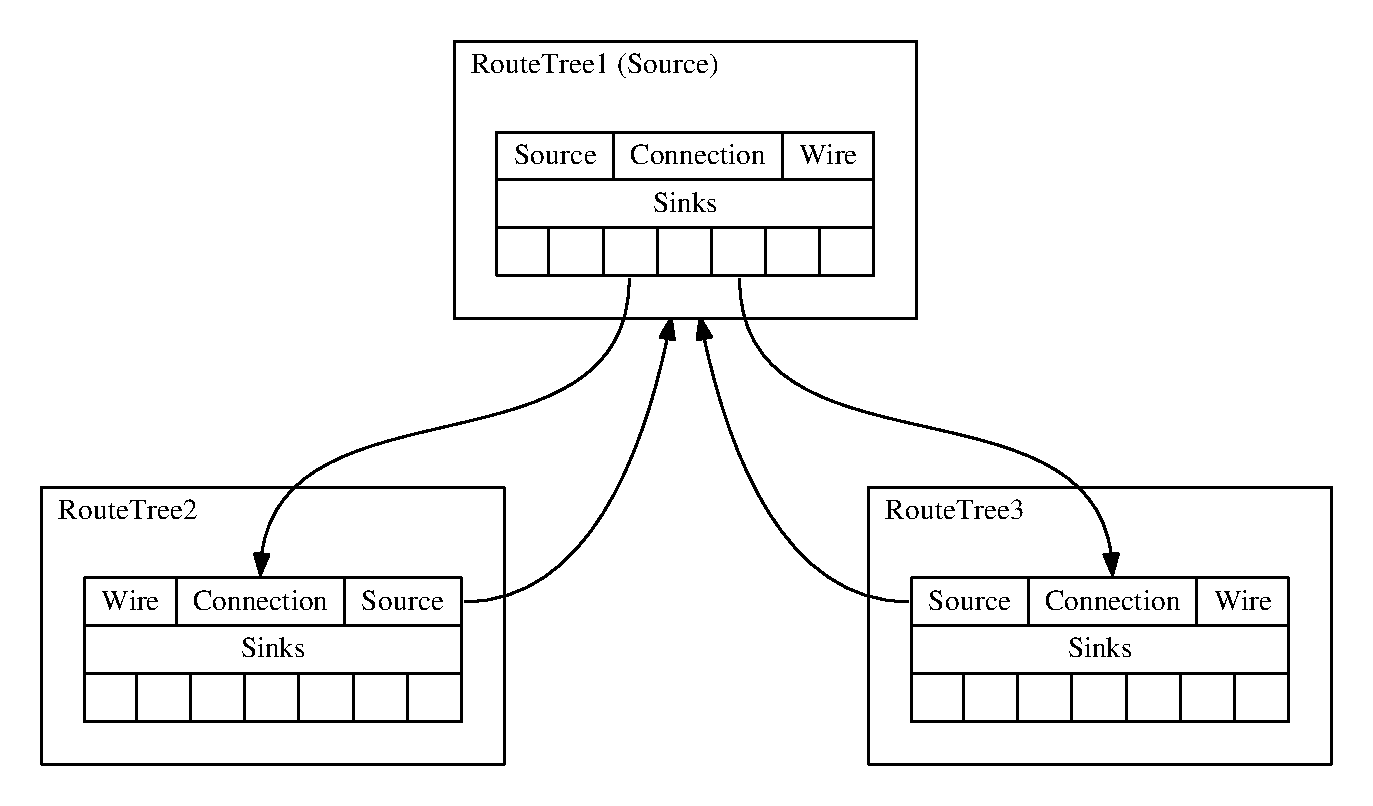
\includegraphics[width=0.8\columnwidth]{routeTreeDS.eps}
\caption{Visual Representation of a RapidSmith2 RouteTree}
\label{fig:routeTreeDS}
\end{figure}

\noindent
As the figure shows, a \texttt{RouteTree} is a simple tree data structure. Each
node in the tree represents a physical wire in the device, and is connected to
other nodes (wires). Edges in the tree represent wire connections (i.e. how one wire
connects to another). A \texttt{RouteTree} can also be conceptually thought of as
a graph, with a single ``starting'' node and several ``sink'' nodes. A
\texttt{RouteTree} node contains the following members:

\begin{figure}[b!]
\centering
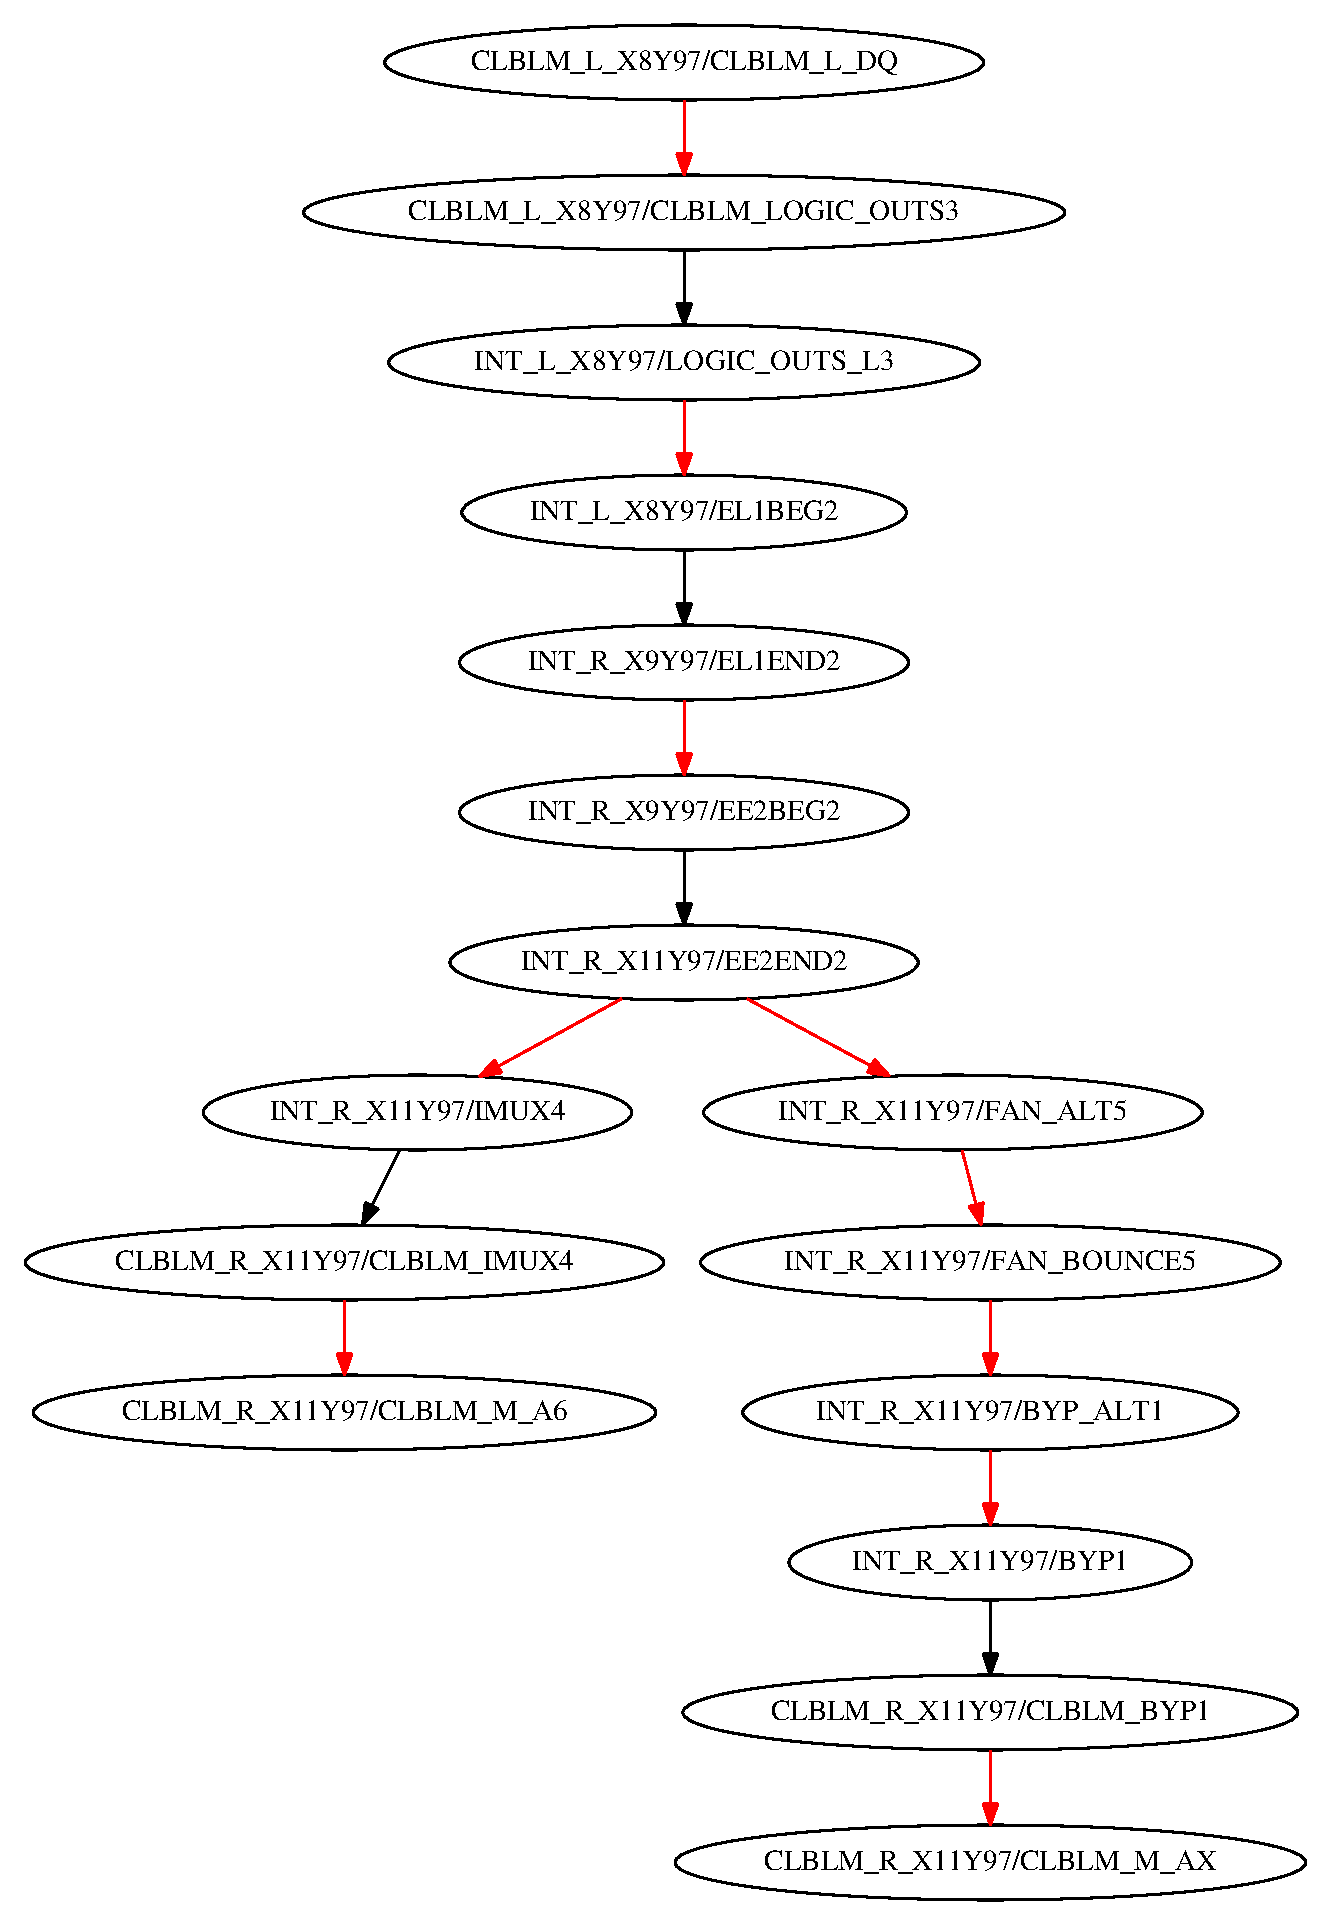
\includegraphics[width=0.65\columnwidth]{routeTree.eps}
\caption{Sample RapidSmith2 RouteTree (red edges represent PIP connections)}
\label{fig:routeTree}
\end{figure}

\begin{itemize}
  \item \textbf{Wire}: The physical \texttt{Wire} object that the \texttt{RouteTree} node
  represents. This can be either a \texttt{TileWire} or \texttt{SiteWire}.
  
  \item \textbf{Source}: A link to the parent \texttt{RouteTree} node
   
  \item \textbf{Connection}: The \texttt{Connection} taken from the \textbf{parent}
  \texttt{RouteTree} node to reach the \textbf{current} \texttt{RouteTree}
  node. In other words, it is the \texttt{Connection} object that was taken
  from the parent wire to reach the current wire.
  
  \item \textbf{Sinks}: A list of child nodes. There is no limit
  to how many children a \texttt{RouteTree} can have.
  
  \item \textbf{Cost} (not shown): An optional cost field for routers 
\end{itemize}

A complete \texttt{RouteTree} specifies how the source of a
\texttt{CellNet} is physically connected to all of its sinks.
\autoref{fig:routeTree} shows an example of a complete \texttt{RouteTree} in
RapidSmith2. As can be seen, the \texttt{CellNet} that is being routed has once
source site pin, and two sink site pins. The source pin is connected to wire
\texttt{CLBLM\_L\_X8Y97/CLBLM\_L\_DQ}, and the sink pins are connected to the
wires \texttt{CLBLM\_R\_X1Y97/CLBLM\-\_M\_A6} and
\texttt{CLBLM\-\_R\_X11Y97/CLBLM\_M\_AX}. Starting from the source, wires are
traversed downward (via wire connections) until the target wires are reached.
\autoref{code:routeTree} demonstrates the basic usage of \texttt{RouteTree}s in
RapidSmith2. The \textbf{DesignAnalyzer}, \textbf{AStarRouter}, and
\textbf{HandRouter} examples in the RapidSmith2 repository also demonstrate
how to traverse and build a \texttt{RouteTree}.

\begin{lstlisting}[xleftmargin=1.5em, framexleftmargin=1.5em, caption=Building a
RouteTree, label=code:routeTree] 
  // Find a Wire to start the RouteTree at
  Site site = device.getSite("SLICE_X5Y84");
  SitePin pin = site.getSitePin("DQ");
  Wire startWire = sink.getExternalWire();

  // Create the first node in the RouteTree 
  Queue<RouteTree> rtQueue = new LinkedList<RouteTree>();
  RouteTree start = new RouteTree(startWire);
  rtQueue.add(start);

  // Build up the RouteTree somehow 
  while (!amDone()) {
	  RouteTree current = rtQueue.poll();
	  Wire wire = route.getWire();

	  for (Connection conn : wire.getWireConnections()) {
		  // add qualified connections to the RouteTree
		  if (isQualified(wire)) {
			  RouteTree tmp = current.addConnection(conn);
			  rtQueue.add(tmp);
		  }
	  }
  }
\end{lstlisting}

When a design is imported from Vivado through a RSCP, the routing information
is parsed and loaded into \texttt{Route\-Tree}s for each \texttt{CellNet}. On
design export, the \texttt{RouteTree} for each \texttt{CellNet} is traversed
and converted into a Vivado \texttt{ROUTE} string. Users can use custom data
structures to route a design, but they needs to be \textbf{converted to an
equivalent RouteTree representation} before exporting the design to Vivado.  

\subsection{Three Part Routing} \label{sec:threePartRouting}
In RapidSmith2, there are three sections to a routed \texttt{CellNet}: 

\begin{enumerate}
  \item The portion of the net that starts at the source BEL pin, and is routed
  to an output site pin. This part of the route exists completely inside of
  site boundaries.
  
  \item The portion of the net that starts at the output site pin of part (1),
  and is routed to several sink site pins. This part of the route is
  called the \textbf{intersite} route because it connects sites together. A
  typical router is responsible for routing this section of the
  net\footnote{VCC and GND nets don't follow this pattern. The only difference
  for VCC and GND is that they can have multiple intersite nets.}.
  
  \item The portion of the net that starts at the sink site pins from part (2),
  and is routed to sink BEL pins. Since there can be several sink pins in a
  \texttt{CellNet}, this section of the net can have more than one component.
  Each component exists completely inside site boundaries.
\end{enumerate}

\noindent \autoref{fig:threePartRouting} shows a visual representation of the
three-part routing structure. Each section of a route has a corresponding
\texttt{RouteTree} object. A source \texttt{RouteTree} represents the orange
wires in the figure (part 1), an intersite \texttt{RouteTree} represents the
green wires in the figure (part 2), and a list of sink \texttt{RouteTree}s
represents the purple wires in the figure (part 3, with a different
\texttt{RouteTree} object for each site). It is important to note that
intrasite nets only have a source \texttt{RouteTree} because they are
completely contained within a site. \autoref{code:threePartRouting} demonstrates
how to utilize three-part routing in RapidSmith2. On design import, the routing
sections of each \texttt{CellNet} are created automatically.

\begin{figure}[t]
\centering
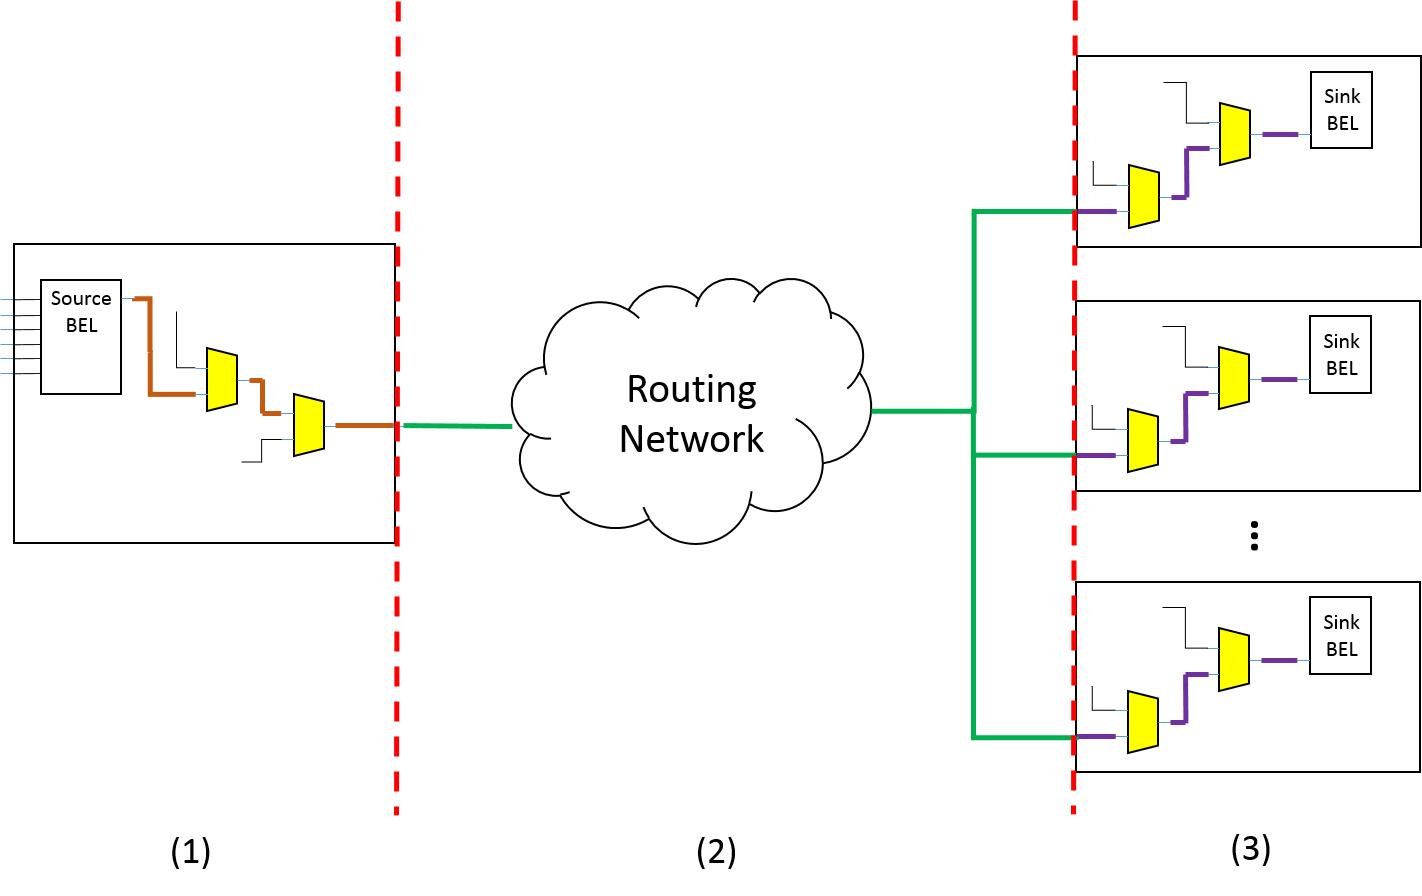
\includegraphics[width=1\columnwidth]{threePartRouting.png}
\caption{Three-Part Routing}
\label{fig:threePartRouting}
\end{figure}

\begin{lstlisting}[xleftmargin=1.5em, framexleftmargin=1.5em,
caption=Demonstration of three-part routing in RapidSmith2,
label=code:threePartRouting] 
  // Get a handle to a routed net in the design 
  CellNet net = design.getNet("myNet");

  // Handling the source RouteTree
  RouteTree source = net.getSourceRouteTree();
  net.setSourceRouteTree(createSourceRoute());

  // Handling the intersite RouteTree
  RouteTree intersite = net.getIntersiteRouteTree();
  net.addIntersiteRouteTree(createIntersiteRoute());

  // Iterate over a list of sink RouteTrees
  for (RouteTree rt : net.getSinkSitePinRouteTrees()) {
	  // do something with the RouteTree
  }

  // Or, get a RouteTree based on a SitePin
  for(SitePin sitePin : net.getSitePins()) {
	  if (sitePin.isInput()) {
		  RouteTree sinkTree = net.getSinkTree(sitePin);
		  // do something with the RouteTree
	  }
  }

  // Add a new sink RouteTree that starts at a SitePin
  net.addSinkRouteTree(sitePin, createSinkRouteTree(sp));
\end{lstlisting}


\subsection{Routing in Vivado}
The reason a three-part routing distinction is necessary in RapidSmith2, is due
to how routing is represented in Vivado. Inside site boundaries, a route is
represented using site PIPs. A string of enabled PIPs determines what pins
are connected together within the site. Between site boundaries, a route is
instead represented using wires. The wires are formatted into a Vivado ROUTE
string, which uniquely specifies the intersite route for a net. The three-part
routing representation makes this distinction explicit to the users of
RapidSmith (it also makes import/export easier). When a design is exported from
Vivado, the intrasite portions of a net are exported as site PIPs, and the
intersite portion of the net is exported as wires.

\begin{lstlisting}[numbers=none, keywordstyle=, stringstyle=]
// An example of a string of used site pips in Vivado
{IUSED:0 IBUFDISABLE_SEL:GND INTERMDISABLE_SEL:GND}

// An example of a Vivado ROUTE string
 { CLBLL_LL_AQ CLBLL_LOGIC_OUTS4  { NW6BEG0 NE2BEG0 WR1BEG1 IMUX_L34
IOI_OLOGIC0_D1 LIOI_OLOGIC0_OQ LIOI_O0 }  IMUX_L1 CLBLL_LL_A3 }
\end{lstlisting}

\subsection{Intrasite Routing}
On design import, the site PIP information extracted from Vivado is stored
into RapidSmith2 data structures, and used to reconstruct the three-part
routing view described in the previous section. This gives the user two options
when dealing with intrasite routing in RapidSmith2: (1) use the three-part
routing data structures, or (2) use the set of enabled site PIPs stored in the
\texttt{CellDesign}. It is user preference for which representation to use
when writing a CAD tool, but both representations need to be up-to-date before
design export. \autoref{code:sitePips} demonstrates how a set of used site PIPs
can be created and added to a site. This step needs to be taken \textbf{only
when you have modified the intrasite routing} for a site.

\begin{lstlisting}[xleftmargin=1.5em, framexleftmargin=1.5em, caption=Code
to transform a set of SiteWires into Site PIPs, label=code:sitePips]
  // Get a handle to a Design and a Site
  CellDesign design = vcp.getDesign();
  Device device = vcp.getDevice();
  Site site = device.getSite("SLICE_X5Y84");

  // Get a list of used site wires somehow (this is up to you)
  Set<Wire> usedSiteWires = getUsedWires(site);

  // Convert the list of wires to their integer enumeration
  Set<Integer> usedPipWires = usedSiteWires.stream()
										 .map(w -> w.getWireEnum())
										 .collect(Collectors.toSet());

  // Set the used site pips with the design class
  design.setUsedSitePipsAtSite(site, usedPipWires);
\end{lstlisting}
%%%%%%%%%%%%%%%%%%%%%%%%%%%%%%%%%%%%%%%%%%%%%%%%%%%%%%%%%%%%%%%%%%%%%%%%%%%%%%%%%%%%%%%%%
% Section 8: Importing RSCPs and exporting TCPs
%	This section contains a description of the following:
%	- The contents of RapidSmith Checkpoints (RSCP)
% 	- How to load a RSCP into RapidSmith2 
%	- The contents of Tincr Checkpoints (TCP)
% 	- How to export a TCP from RapidSmith2 
%	- Important information that is imported from RSCP and how they are
% 		represented in RS2 (such as routethroughs) 	
%	- Code samples for importing RSCPs and exporting TCPs
%%%%%%%%%%%%%%%%%%%%%%%%%%%%%%%%%%%%%%%%%%%%%%%%%%%%%%%%%%%%%%%%%%%%%%%%%%%%%%%%%%%%%%%%%
\newpage
\section{Design Import/Export} \label{sec:import}
Importing and exporting designs between Vivado and RS2 is fairly
straightforward. It is done using Tincr Checkpoint (TCP) files, which contain a
variety of information about a digital design. This section describes in detail
the following: 

\begin{itemize}
  \item The contents of TCP files
  \item The small differences between TCP files for design import and export
  \item How to load a TCP into RS2, and how to export a RS2 design to a TCP
  \item Some additional information that is imported with a TCP 
\end{itemize}

\subsection{RapidSmith Checkpoints}
RapidSmith checkpoints (RSCP) are Tincr checkpoints generated in Vivado from the
command \texttt{::tincr::write\-\_rscp}. These checkpoints are capable of
representing a Vivado design at any stage of implementation (post-synthesis,
post-place, and post-route), and can be parsed and imported into RapidSmith. As
we will see in \autoref{sec:tcp} below, the format of these checkpoints differ
slightly than those of regular TCPs. This is because a great deal of additional
information needs to be added to RapidSmith checkpoints in order to import a
complete representation of a Vivado design. The remainder of this subsection
describes each of the file types within a RapidSmith checkpoint, and what they
represent.

\subsubsection{design.info}
The \textit{design.info} file within a RSCP is used to include any useful
information about a design. Currently, it only stores the part name that the
design is implemented on. This file is reserved to add more additional
information in the future.

\subsubsection{netlist.edf}
The \textit{netlist.edf} file within a RSCP is an EDIF netlist representing the
logical portion of a design. It details all of the \cells, \nets,
and \ports within a design, and is generated from Vivado using the Tcl
command \texttt{write\_edif}. A RapidSmith \celldesign is created by parsing the
EDIF file, and converting it into the appropriate RS2 data structures described
in \autoref{sec:designDS}. Below is an example of a RSCP EDIF file.

\begin{lstlisting}[numbers=none, keywordstyle=, stringstyle=]
  (Library work
    (edifLevel 0)
    (technology (numberDefinition ))
   (cell add (celltype GENERIC)
     (view add (viewtype NETLIST)
       (interface 
        (port a (direction INPUT))
        (port b (direction INPUT))
        (port cin (direction INPUT))
        (port cout (direction OUTPUT))
        (port s (direction OUTPUT))
       )
       (contents
         (instance GND (viewref netlist (cellref GND (libraryref hdi_primitives))))
         (instance VCC (viewref netlist (cellref VCC (libraryref hdi_primitives))))
         (instance a_IBUF_inst (viewref netlist (cellref IBUF (libraryref hdi_primitives))))
         (instance b_IBUF_inst (viewref netlist (cellref IBUF (libraryref hdi_primitives))))
         (instance cin_IBUF_inst (viewref netlist (cellref IBUF (libraryref hdi_primitives))))
         (instance cout_OBUF_inst (viewref netlist (cellref OBUF (libraryref hdi_primitives))))
         (instance cout_OBUF_inst_i_1 (viewref netlist (cellref LUT3 (libraryref hdi_primitives)))
           (property INIT (string "8'hE8"))
         )
\end{lstlisting}

\subsubsection{placement.rsc}
The \textit{placement.rsc} file within a RSCP stores all of the placement
information of a Vivado design. This includes which package pin every \port is
mapped to, which \bel each \cell is placed on, and the logical-to-physical pin
mappings for each \cellpin. If a design has not yet been placed, this file
will be empty. Below is an example of a RSCP placement file.

\begin{lstlisting}[numbers=none]
LOC a_IBUF_inst R10 IOB33 INBUF_EN LIOB33_SING_X0Y50
PINMAP a_IBUF_inst O:OUT I:PAD 
LOC b_IBUF_inst T10 IOB33 INBUF_EN LIOB33_X0Y51
PINMAP b_IBUF_inst O:OUT I:PAD 
LOC cin_IBUF_inst T9 IOB33 INBUF_EN LIOB33_X0Y51
PINMAP cin_IBUF_inst O:OUT I:PAD 
LOC cout_OBUF_inst U13 IOB33 OUTBUF LIOB33_X0Y53
PINMAP cout_OBUF_inst O:OUT I:IN 
LOC cout_OBUF_inst_i_1 SLICE_X0Y51 SLICEL A6LUT CLBLL_L_X2Y51
PINMAP cout_OBUF_inst_i_1 O:O6 I0:A4 I1:A5 I2:A6 
LOC s_OBUF_inst T13 IOB33 OUTBUF LIOB33_X0Y53
PINMAP s_OBUF_inst O:OUT I:IN T:TRI 
PACKAGE_PIN R10 a
PACKAGE_PIN T10 b
PACKAGE_PIN T9 cin
PACKAGE_PIN U13 cout
PACKAGE_PIN T13 s
\end{lstlisting}

\subsubsection{routing.rsc}
The \textit{routing.rsc} file within a RSCP stores all of the routing
information of a Vivado design. This includes: 

\begin{itemize}
  \item The used \cls{Site} \cls{PIPs} within each \cls{Site} (which
  specifies the internal routing)
  \item A list of LUT \bels that are acting as static sources (see
  \autoref{sec:additionalInfo} for more details)
  \item A list of LUT \bels that are being used as routethroughs (see
  \autoref{sec:additionalInfo} for more details) 
  \item The name of each INTRASITE net
  \item The name, connecting \cls{SitePin}s, and used \cls{TileWire}s
  of each INTERSITE net.
  \item Special routing information for the VCC and GND nets.
\end{itemize}

\noindent
If Vivado has not yet been routed, this file will be mostly empty. Below is
an example of the contents within a RSCP routing file.

\begin{lstlisting}[numbers=none]
SITE_PIPS SLICE_X9Y80 SRUSEDMUX:0 CEUSEDMUX:IN COUTUSED:0 CLKINV:CLK DCY0:DX ...
SITE_PIPS SLICE_X13Y80 PRECYINIT:AX SRUSEDMUX:0 CEUSEDMUX:IN COUTUSED:0 ...
SITE_PIPS SLICE_X15Y80 SRUSEDMUX:0 CEUSEDMUX:IN COUTUSED:0 CLKINV:CLK DCY0:DX ...
SITE_PIPS M17 OUSED:0 

... 

STATIC_SOURCES SLICE_X2Y106/D6LUT/O6 SLICE_X2Y106/C6LUT/O6 SLICE_X4Y106/D6LUT/O6 ...
LUT_RTS SLICE_X5Y101/B6LUT/A6/O6 SLICE_X2Y100/A5LUT/A4/O5 SLICE_X5Y100/C6LUT/A6/O6 ...

...

INTRASITE AddSub[10]
INTERSITE AngStep1[0] SLICE_X2Y82/AX SLICE_X2Y87/AQ SLICE_X2Y84/A1
ROUTE AngStep1[0] CLBLM_R_X3Y87/CLBLM_M_AQ CLBLM_R_X3Y87/CLBLM_LOGIC_OUTS4 ...

...

VCC INT_L_X2Y107/VCC_WIRE INT_L_X2Y107/VCC_WIRE INT_L_X2Y107/VCC_WIRE ...
START_WIRES INT_L_X2Y107/VCC_WIRE INT_L_X2Y106/VCC_WIRE INT_R_X3Y106/VCC_WIRE ...
GND INT_R_X3Y106/GND_WIRE INT_R_X3Y106/GND_WIRE INT_R_X3Y106/GFAN1 ...
START_WIRES INT_R_X3Y106/GND_WIRE INT_L_X4Y106/GND_WIRE INT_R_X3Y105/GND_WIRE ...
\end{lstlisting}

\subsubsection{contraints.rsc}
The \textit{contraints.rsc} file within a RSCP stores all XDC constraints on a
Vivado design. XDC constraints are similar to UCF files for ISE designs. They
can be used to set the clock frequency, constrain a top-level port to a specific
package pin on the device, and set other physical implementation details. An
example of a RSCP constraints file can be seen below.

\begin{lstlisting}[numbers=none]
create_clock -period 5.000 -name sysClk -waveform {0.000 2.500}
set_property IOSTANDARD LVCMOS18 [get_ports clk]
set_property IOSTANDARD LVCMOS18 [get_ports ena]
set_property PACKAGE_PIN E15 [get_ports {Yin[12]}]
set_property PACKAGE_PIN H17 [get_ports {Xin[14]}]
set_property PACKAGE_PIN D18 [get_ports {Xin[7]}]
\end{lstlisting}

\noindent
As can be seen, a Vivado constraints file is essentially a list of Tcl commands
to execute before generating a bitstream. When importing a RSCP into RapidSmith,
each constraint is parsed into a \cls{XdcConstraint} object and stored in the
top-level \celldesign. Each \cls{XdcConstraint} has two fields, a String
command and a String representing all command arguments. \autoref{code:xdc}
demonstrates how to manipulate XDC constraints in RapidSmith. Future RS2 plans
include creating a more intelligent way of handling XDC constraints. 

\begin{lstlisting} [caption=How to manipulate XDC constraints in RS2,
label=code:xdc] 
// Getting a list of all constraints in the current design
List<XdcConstraint> xdcConstraints = design.getVivadoConstraints();

// Look for all of the "create_clock" constraints in the design
List<XdcConstraint> crtClks = xdcConstraints.stream()
                              .filter(xdc -> xdc.getCommandName().equals("create_clock")) 
                              .collect(Collectors.toList());

// Add a new XDC constraint to the design
XdcConstraint xdc = new XdcConstraint("set_property", "IOSTANDARD LVCMOS18 [get_ports clk]") 
design.addVivadoConstraint(xdc);
\end{lstlisting}

\subsubsection{macros.xml}

The \textit{macros.xml} file within a RSCP contains template information about
macro cells in a Vivado design that (a) were not fully flattened, and (b) do not
exist in the default Vivado cell library. Using the information in the XML file,
a \cls{LibraryCell} can be created and added to the \cls{CellLibrary} so that
the design can import correctly. More information about macro cells in
RapidSmith can be found in \autoref{sec:macros}.

\begin{lstlisting}[numbers=none]
<?xml version="1.0" encoding="UTF-8"?>
<root>
  <macros>
    <macro>
        <type>IOBUF</type>
        <cells>
            <internal>
                <name>IBUF</name>
                <type>IBUF</type>
            </internal>
            <internal>
                <name>OBUFT</name>
                <type>OBUFT</type>
            </internal>
        </cells>
        <pins>
            <pin>
                <name>IO</name>
                <direction>inout</direction>
                <type>MACRO</type>
                <internalConnections>
                    <pinname>IBUF/I</pinname>
                    <pinname>OBUFT/O</pinname>
                </internalConnections>
            </pin>
            ...
        </pins>
    </macro>
  </macros>
</root>  
\end{lstlisting}


\subsection{Tincr Checkpoints} \label{sec:tcp}
Tincr checkpoints are very similar to RapidSmith checkpoints, but they can be
used to import designs back into Vivado after they have been modified in
RapidSmith. The main different between TCPs and RSCPs, is that the
\textit{placement.rsc}, \textit{routing.rsc}, and \textit{constraints.rsc} files
turn into \textit{placement.xdc}, \textit{routing.xdc}, and \textit{constraints.xdc}
respectively. Vivado is able to parse the XDC files and apply physical
information to the design. On design export, RapidSmith produces
a TCP that is compatible with Vivado. The file formats of the three XDC files
will not be included in this documentation. If you are interested in their
format, the best way to learn is to consult the Vivado user guide and generate a
TCP from RapidSmith and view the individual files.

\subsection{Additional Information} \label{sec:additionalInfo}
The reason RSCP and TCP checkpoints are distinguished, is that there are
several design implementation aspects in Vivado that aren't explictly
represented. In order to accurately represent a design in RapidSmith, they
must be included somehow. This section describes the parts of the design that
aren't explicitly represented in Vivado, and how RapidSmith handles them.
\autoref{sec:importExportTcp} describes how to get a handle to the additional
information after a checkpoint has been imported.

\subsubsection{LUT Routethroughs}
Besides their use in implementing logic equations, LUT BELs can also act as
signal routethroughs. In Vivado, a LUT is marked as a  routethrough when its
configuration equation (CONFIG.EQN) maps the value of a single input pin
directly to the output pin. These LUTs are not explicitly represented in the
logical netlist because there is no cell placed on the corresponding BEL. 
\autoref{fig:routethroughs} shows two examples of LUTs in Vivado that are
configured as routethroughs.

\begin{figure}[h]
  \centering
  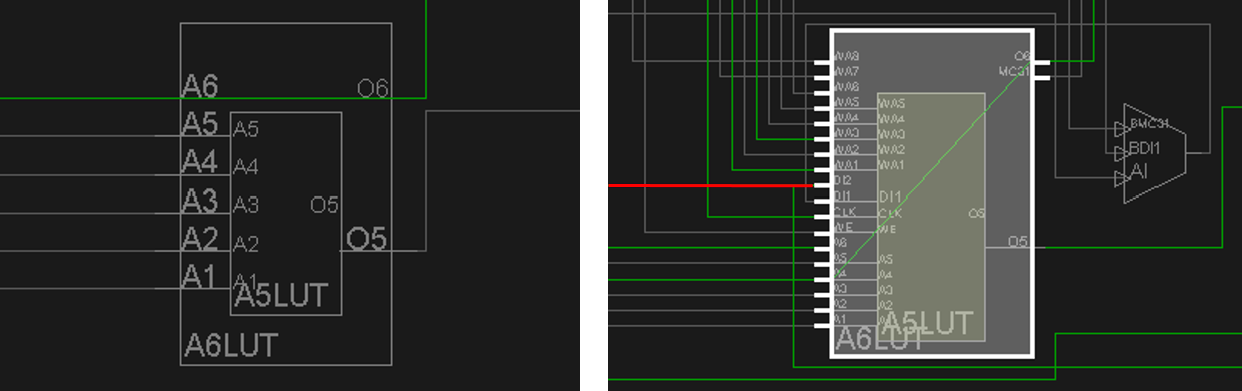
\includegraphics[width=1\columnwidth]{routethroughs}
  \caption{Two examples of LUTs being used as
  routethroughs in the Vivado GUI. The RT on the left uses the A6 input pin,
  while the RT on the right uses the A4 input pin. The net highlighted in red
  represents VCC.}
  \label{fig:routethroughs}
\end{figure}

\noindent
When a design is exported from Vivado, all LUTs that are acting as routethroughs
are included in the \textit{routing.rsc} file of a RSCP. When the file is
parsed, each routethrough is stored in a \cls{BelRoutethrough} object which
contains the physical \bel, the input \belpin, and the output \belpin that
uniquely describes the routethrough. It is important to note that if a \bel is
being used as a routethrough, no \cell can be placed there. When creating CAD
tools, \cls{BelRoutethrough}s give the user a more complete picture of what
\bels are actually available. 
	
As described in \autoref{otherConns}, there is a \cls{Connection} object in
RapidSmith from every input LUT pin to the LUTs output pin. These \bel
routethrough connections, are actually just \cls{WireConnection}s with the
\texttt{isRoute\-through()} method returning true. In order to use a LUT as a
routethrough in RapidSmith, you simply have to include the corresponding
\cls{WireConnection} within an INTRASITE \cls{RouteTree}. When a design is
exported from RapidSmith, the routethrough \cls{WireConnection}s are
automatically detected and converted to a passthrough LUT \cell. The netlist
is rewired appropriately.

\subsubsection{Static Source LUTs}
LUTs can also act as a static power or ground source. This occurs when the
configuration equation is set to 1 or 0. An example of a LUT that exhibits
this behavior is shown in \autoref{fig:staticSourceLut}. When a design
is exported from Vivado, all LUTs that are acting as static sources are
included in the \textit{routing.rsc} file of a RSCP. As the file is being
parsed, a list of static sources \bels are recorded and stored in a list data
structure. Just like routethroughs, if a \bel is being used as a static source
no \cell should be placed on it.

\begin{figure}[h]
  \centering
  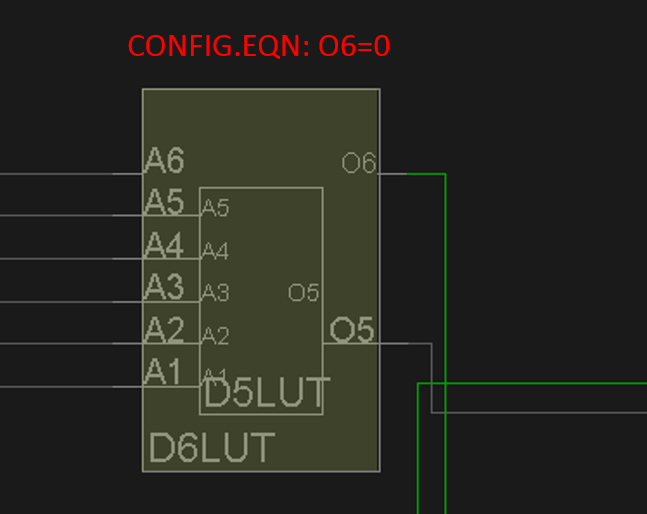
\includegraphics[width=.5\columnwidth]{staticSourceLut.png}
  \caption{A LUT \bel that has been configured as a GND source. Notice that
  there are no input pins being driven.}
  \label{fig:staticSourceLut}
\end{figure}

\subsubsection{Pseudo CellPins}
\cls{PseudoCellPin}s are described in great detail in \autoref{sec:cellPin}.
When a RSCP is loaded, \cls{PseudoCellPin}s are automatically detected,
created, and attached to their corresponding \cells.

\subsection{Importing RSCPs and Exporting TCPs} \label{sec:importExportTcp}
After a Vivado design has been converted to a RSCP using the
\texttt{::tincr::write\_rscp} command, it can be loaded into RapidSmith.
\autoref{code:import} demonstrates the basix syntax of design
import and export.

\begin{lstlisting}[caption=How to import and export TCP files to and from RS2,
label=code:import]
// Loading a Tincr Checkpoint
TincrCheckpoint tcp = VivadoInterface.loadTcp("pathToCheckpoint.tcp");
CellDesign design = tcp.getDesign();
Device device = tcp.getDevice();
CellLibrary libCells = tcp.getLibCells();

// Insert CAD Tool Here

// Exporting the modified design to a Tincr Checkpoint
VivadoInterface.writeTCP("pathToStore.tcp", design, device, libCells);

\end{lstlisting}

\noindent
While a design is being imported into RapidSmith, several useful data structures
are built up. If you want to gain access to those data structures, you can pass
an additional argument into the \texttt{VivadoInterface.loadTCP} method. This
is shown in \autoref{code:import2}.

\begin{lstlisting}[caption=Importing a TCP with additional information,
label=code:import2]
// Loading a Tincr Checkpoint with additional info
TincrCheckpoint tcp = VivadoInterface.loadTcp("PathToCheckpoint.tcp", true);
Collection<BelRoutethrough> belRts = tcp.getRoutethroughObjects();
Collection<Bel> staticSources = tcp.getStaticSourceBels();
Map<BelPin, CellPin> belPinToCellPinMap = tcp.getBelPinToCellPinMap()
\end{lstlisting}

\noindent
After a design is exported from RapidSmith, a Tincr Checkpoint (TCP) is
produced. To import the TCP back into Vivado, simply open up Vivado in Tcl mode
and use the following command:

\begin{code}
Vivado% tincr::read_tcp myCheckpoint.tcp
\end{code}
%%%%%%%%%%%%%%%%%%%%%%%%%%%%%%%%%%%%%%%%%%%%%%%%%%%%%%%%%%%%%%%%%%%%%%%%%%%%%%%%%%%%%%%%%
% Section 9: Example Programs
%	This section describes several example programs in the RapidSmith2 repository that
%	can be used to learn how to use RapidSmith2.
%%%%%%%%%%%%%%%%%%%%%%%%%%%%%%%%%%%%%%%%%%%%%%%%%%%%%%%%%%%%%%%%%%%%%%%%%%%%%%%%%%%%%%%%%
\newpage
\section{Example Programs} \label{examples}
\graphicspath{{./techReportFigures/sec9_examples/}}

A variety of example programs can be found in the
\pkg{edu.byu.edu.rapidSmith.examples} package of the RapidSmith2 installation.
They have been heavily commented to provide a means to learn the RapidSmith2 API by
example. We believe this approach is better than reading through a block of
text while trying to understand the data structures and what they do.
There is a \fil{README.txt} file in that directory to provide an overview of
each example. The order that they appear in the \fil{README.txt} is also the
suggested learning order for beginners. In addition, the subsections below
describe one or more built-in RapidSmith2 programs which you might find useful.

\subsection{Sample Vivado Designs}
To enable new users of RapidSmith2 to quickly start running the example
programs, a small set of pre-compiled Vivado designs have been included in the
distribution. They are located in the \dir{exampleVivadoDesigns} directory of
the repository, and consist of 3 designs: 
\begin{itemize}
\item \textbf{add.rscp}: synthesized only
\item \textbf{cordic.rscp}: synthesized and placed
\item \textbf{count16.rscp}: synthesized, placed and routed
\end{itemize} 
Equivalent Vivado checkpoints files (.dcp) are also included in
the same directory as \fil{add.dcp}, \fil{cordic.dcp}, and \fil{count16.dcp}
files. To open these checkpoints in Vivado, you can either (a) double click on
the .dcp file in a file explorer, or (b) use the command
\texttt{open\_checkpoint} when a Vivado terminal is open. It is suggested that
you have the equivalent Vivado designs open when going through the example
programs listed below.

If you want to recompile the designs from scratch, the source code for each
design has also been included in the same directory. The Tcl script called
\pgm{compile.tcl} can be used for this purpose. Simply open Vivado in Tcl
mode, and type the Tcl commands shown in \autoref{lst:compilation} to re-compile
and implement one of the example designs. This will synthesize, place, and
route a design and, from that compiled design, generate the \dir{.rscp}
directory and the \fil{.dcp} file. For example programs that only explore the
architecture, opening the device browser in Vivado can also be helpful.
                 
\begin{lstlisting} [numbers=none,keywordstyle=\ttfamily, caption=Sample
Tcl commands to run the Vivado compilation script, label=lst:compilation] 
	Vivado% cd <path to exampleVivadoDesigns directory>
	Vivado% source compile.tcl
	Vivado% compile_hdl_to_checkpoint_files add
	Vivado% close_project
\end{lstlisting}

\subsection{\pgm{DeviceBrowser}}
The DeviceBrowser is a GUI program located in the 
\pkg{edu.byu.ece.rapidSmith.device.browser} package. It lets you browse
parts at the tile level, and is useful for becoming more familiar with FPGA
architecture. As long as a valid device file exists, then the DeviceBrowser can
operate (no design required). A screenshot from the DeviceBrowser can be seen in
\autoref{fig:deviceBrowser}. On the left, the user may choose the desired part
by navigating the tree menu and double-clicking on the desired part name.
This will load the part in the viewer pane on the right (the first available
part is loaded at startup). The status bar in the bottom left displays which
part is currently loaded. Also displayed is the name of the current tile
which the mouse is over, highlighted by a yellow outline in the viewer pane.
The user may navigate inside the viewer pane by using the mouse. By
right-clicking and dragging the cursor, the user may pan. By using the
scroll-wheel on the mouse, the user may zoom. If a scroll-wheel is
unavailable, the user may zoom by clicking inside the viewer pane and pressing
the minus(-) key to zoom out or the equals(=) key to zoom in.

\begin{figure}[htb]
\centering
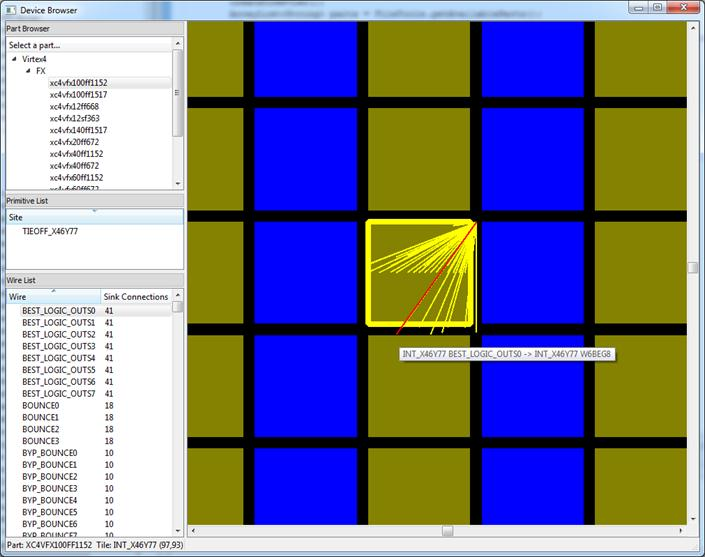
\includegraphics[width=0.8\columnwidth]{deviceBrowser2.jpg}
\caption{\pgm{DeviceBrowser} Screen Shot Showing Wire Connections}
\label{fig:deviceBrowser2}
\end{figure}

The device browser also allows the user to follow the various connections found
in the FPGA.  By double clicking a wire in the wire list, the application will
draw the connection on the tile array (as shown in
\autoref{fig:deviceBrowser2}). By hovering the mouse pointer over the
connection, the wire becomes red and a tooltip will appear describing the
connection made by declaring the source tile and wire followed by an arrow and
the destination tile and wire.  By clicking on the wire, the application will
redraw all the connections that can be made from the currently selected wire. 
By repeating this action, the user can follow connections and discover how the
FPGA interconnect is laid out. Thanks to Chris Lavin for originally creating
this application.

\subsection{\pgm{DeviceAnalyzer}}
The DeviceAnalyzer is designed as a simple getting started program and
demonstrates how to use some of the Device data structures in RapidSmith2. This
includes how to query for and print tiles in a device, how to use wires and
wire connections, and other useful device functions.

\subsection{\pgm{ImportExportExample}} \label{sec:importExportExample}
The ImportExportExample demonstrates how to load a RapidSmith Checkpoint
(RSCP) into RapidSmith2, and how to export a RapidSmith2 design back into a Tincr
Checkpoint (TCP). This is a very important step in passing digital designs back
and forth between Vivado and RapidSmith2.

\subsection{\pgm{DesignAnalyzer}}
The DesignAnalyzer loads a RapidSmith Checkpoint into RapidSmith2, walks
the design data structures, and prints what it finds as it goes in a
readable format. As such, it provides a nice example of a number of things which would
be useful for getting started with RapidSmith2 including:
\begin{itemize}
  \item How to enumerate the Cells in a design, determine and print their 
  placement information, and determine and print their properties.
  \item How to enumerate the logical nets in a design and print out their source
  and sink pins. 
  \item How to traverse and print out the physical route for a logical net (if
  it is routed)  
\end{itemize}

\subsection{CreateDesignExample} \label{sec:createDesignExample}
The CreateDesignExample program builds a RapidSmith2 netlist from scratch (using
\cells and \cellnets) and then places the design. While this is certainly not
recommended for substantial designs, it does demonstrate how to do the
following useful tasks in RapidSmith2:

\begin{itemize}
  \item Create new \cells and add them to an existing netlist
  \item Create new \cellnets, and connect them to \cls{CellPin}s
  \item Modify the properties on \cells
  \item Place \cells onto a \bels
  \item Find compatible \bel placement for a given \cell
\end{itemize}

\subsection{Other Test Programs}
The programs introduced in this section are designed for beginners of RapidSmith2. Once
you start becoming more comfortable with RapidSmith2 and its data structures,
there are several other more advanced examples. These examples include the
\pgm{HandRouter}, \pgm{AStarRouter}, and \pgm{SimulatedAnnealingPlacer}
programs. See the README.txt file for more information about each of these
examples.

%%%%%%%%%%%%%%%%%%%%%%%%%%%%%%%%%%%%%%%%%%%%%%%%%%%%%%%%%%%%%%%%%%%%%%%%%%%%%%%%%%%%%%%%%
% Section 10: Installing New Devices
%	This section provides a detailed walkthrough on how to install new devices
%	to be used in RapidSmith2.
%%%%%%%%%%%%%%%%%%%%%%%%%%%%%%%%%%%%%%%%%%%%%%%%%%%%%%%%%%%%%%%%%%%%%%%%%%%%%%%%%%%%%%%%%
\newpage
\section{Installing New Device Files} \label{sec:installingNewDevices}
\graphicspath{{./techReportFigures/sec10_deviceInstallation/}}

The device files included with the RapidSmith2 installation (listed in
Section~\ref{sec:supportedDevices}) have been well-tested, and are great starting
points for new users. If you are new to RapidSmith2, it is \textit{strongly
encouraged} to start with these existing device files. However, RapidSmith2
also supports installing new devices for parts not listed in
Section~\ref{sec:supportedDevices}. To create a new RapidSmith2 device
file, four \texttt{Tincr} intermediate files are required:

\begin{enumerate}
  \item XDLRC
  \item Family Info XML
  \item Device Info XML
  \item Cell Library XML
\end{enumerate}

\noindent The contents and format of these files are described in
great detail in Appendix~\ref{sec:appendixXDLRC}, Appendix~\ref{sec:familyInfo},
Appendix~\ref{sec:deviceInfo}, and Section~\ref{sec:cellLibraryinDesignSection}
respectively, and will not be described here. For those that are curious about
what each file represents, refer to the listed appendices. The remainder of this
section documents the required steps to transform the \texttt{Tincr}
intermediate files into compact device files that can be loaded into
RapidSmith2.

\subsection{Creating New Device Files for Supported Families}
\label{sec:creatingNewSupportedDevices} 
Section \ref{sec:supportedDevices} gives a list of currently supported
families in RapidSmith2. If the device to install is \textbf{not} within a
supported family, see Section~\ref{sec:newFamilies} for how to add support for a
new family in RapidSmith2. Otherwise, a new device file can be added in five
easy steps:

\begin {enumerate}
\item Open Vivado in Tcl mode, and execute the \texttt{Tincr} command
\texttt{[::tincr::write\_xdlrc]}. An example usage is shown in
\autoref{lst:apdxAwriteXdlrc} for the Artix7 part \textit{xc7a100tcsg324-3}. The
``-max\_processes'' option is used to parallelize the operation so that it will
execute faster. This Tcl command can take a very long time to run (more than 24
hours for very large devices), and so running the command on a remote machine is
good practice. Be aware that these XDLRC files are massive, and 100 GB for the
largest XDLRC files is not uncommon. Make sure there is enough space on the
hard drive before generating the XDLRC for a device.  NOTE: we have observed
that on some machines the use of more than one process to generate the XDLRC
file may hang.  If this happens, re-run using a ``-max\_processes'' of 1.  

\end {enumerate}

\begin{lstlisting}[numbers=none, caption=XDLRC Generation Example, label=lst:apdxAwriteXdlrc] 
::tincr::write_xdlrc -part xc7a100tcsg324-3 -max_processes 4 -primitive_defs xc7a100tcsg324_full.xdlrc
\end{lstlisting}

\begin{enumerate}
\setcounter{enumi}{1} 
\item Run the \texttt{Tincr} command \texttt{[tincr::create\_xml\_device\_info]}
 to create a \textit{deviceInfo.xml} file for the part. Copy the generated
 \textit{deviceInfo.xml} file to the directory
 \textit{RapidSmithPath/devices/family}, where ``RapidSmithPath'' is the path to
 your RapidSmith2 installation and ``family'' is the corresponding Vivado
 family name (i.e. artix7, kintex7, virtex7, zynq, kintexu, virtexu,
 kintexuplus, virtexuplus, etc.)..

\item Run the device installer in RapidSmith2 and pass the newly created XDLRC
as an argument. An example command line usage is shown in
\autoref{lst:apdxAInstaller}. The device installer creates compact device files
that represent a Xilinx device from the XDLRC and \textit{deviceInfo.xml}
generated in the previous steps. Notice the two JVM command line arguments used
in the command. The first option (``-ea'') enables assertions for the code. It
is important to include this flag so that device file errors can be caught
during parsing. The second option (``-Xmx4096m'') sets how much memory the JVM
can use while running the installer. Since XDLRC files are quite large, the
memory usage of the installer grows very quickly. If the device installer fails
with an out of memory exception, you will need to increase the memory and
re-run the installer (up to 32 GB of memory may be required).
\end{enumerate}

\begin{lstlisting}[numbers=none, caption=RapidSmith2 device installer example
usage, label=lst:apdxAInstaller] 
java -ea -Xmx4096m edu.byu.ece.rapidSmith.util.Installer --generate file xc7a100tcsg324_full.xdlrc
\end{lstlisting}

\begin{enumerate}
\setcounter{enumi}{3}
\item Run the family builder in RapidSmith2 and pass the name of the newly
created part as a command line argument. An example usage is shown in
\autoref{lst:apdxAFamilyBuilder} for an Artix7 device. An \texttt{Artix7.java}
file (or whatever family your device is in) will already exist, but will be
updated with new sites and tile types from the newly installed part.

\item The final step is to create a \textit{cellLibrary.xml} file, which details
all Xilinx primitives that can target the device. Section~\ref{sec:cellLibraryGeneration}
demonstrates how to generate a new cell library. Copy the generated cell library
to the corresponding family folder of the device and rename it to
``cellLibrary.xml.''

\end{enumerate}

\begin{lstlisting}[numbers=none, caption=Family builder example usage,
label=lst:apdxAFamilyBuilder] 
java edu.byu.ece.rapidSmith.util.FamilyBuilders xc7a100tcsg324
\end{lstlisting}

\vspace{.3cm}

\noindent Once the device installer is done executing, the compact devices files
are stored in the corresponding family directory of the RapidSmith2 ``devices''
folder. For example, the device files generated from the example part
\textit{xc7a100tcsg324-3} are stored in the ``artix7'' sub-directory.
\autoref{lst:apdxADeviceFiles} shows the two device files that are created
after the device installer is run. The file ending in ``\_db.dat'' contains the
serialized \texttt{Device} data structures for RapidSmith2. The file ending in
``\_info.dat'' contains additional serialized data (such as reverse wire
connections) that can be optionally loaded with the device.

\begin{lstlisting}[numbers=none, caption=Generated RapidSmith2 device files,
label=lst:apdxADeviceFiles] 
[ttown523@CB461-EE09968:artix7] ls
cellLibrary.xml familyInfo.xml |\textbf{xc7a100tcsg324\_db.dat}| |\textbf{xc7a100tcsg324\_info.dat}|
\end{lstlisting} 

\subsection{Supporting New Device Families} \label{sec:newFamilies}
Vivado 2016.2 supports implementing FPGA designs on devices for the following
families (also called architectures):

\begin{multicols}{2}
	\begin {itemize}
	  \item \textbf{Artix7 (artix7)}
	  \item \textbf{Kintex7 (kintex7)}
	  \item \textbf{Virtex7 (virtex7)}
	  \item \textbf{Zynq (zynq)}
	  \item \textbf{Kintex Ultrascale (kintexu)}
	  \item \textbf{Virtex Ultrascale (virtexu)}
	  \item Kintex Ultrascale+ (kintexuplus)
	  \item Virtex Ultrascale+ (virtexuplus)
	\end{itemize}
\end{multicols}

\noindent The name in parentheses is the Vivado Tcl name for the family. Bolded
items are families that are currently supported in RapidSmith2 and
\texttt{Tincr}. To add RapidSmith2 support for another Vivado family, follow the
steps listed below. \textbf{NOTE: In general, you should not be adding support
for a new family as a general user of RapidSmith2. Instead, create an issue at the
RapidSmith2 GitHub repository and the maintainers of RapidSmith2 in the BYU CCL
lab will work to add support. Thus, the following instructions are intended
mainly for BYU researchers}.

\begin {enumerate}
  \item Create the primitive definitions of the family using VSRT. The VSRT user
  guide is given in located at {\color{blue}\url{
  https://github.com/byuccl/RapidSmith2/tree/master/doc}}.
  
  \item Copy the primitive definitions created in step (1) to the
   directory \textit{tincrPath/cache/family/primitive\_defs}, where
   ``tincrPath'' is the path to your \texttt{Tincr} installation and ``family''
   is the Vivado Tcl name for the family of the primitive defs just generated
   (shown in parentheses above).
   
   \item Create the \textit{familyInfo.xml}. To do this, open Vivado in Tcl mode
   and run the command \texttt{[::tin\-cr::create\-\_xml\_family\_info]}. An
   example usage of the command is shown in \autoref{lst:apdxAFamilyInfo} for
   Kintex UltraScale. As the listing shows, there are three arguments to the
   command:
   
	\begin{itemize}
	  \item \textbf{familyInfo.xml}: The file name to store the generated family
	  info. The file ending ``.xml" will be appended if it is not included.
	  \item \textbf{kintexu}: The Vivado family name.
	  \item \textbf{addedBels.txt} (Optional): The ``addedBels.txt" file that was
	  created during step (1). This file contains a list of added VCC/GND BELs for
	  each family.
	\end{itemize}    
\end{enumerate}

\begin{lstlisting}[numbers=none, caption=Family info example usage, label=lst:apdxAFamilyInfo] 
::tincr::create_xml_family_info familyInfo.xml kintexu addedBels.txt 
\end{lstlisting}


\begin{enumerate}
\setcounter{enumi}{3}    
    \item Modify the generated family info with a few hand edits. The
    current required hand edits are broken down between Series7 and UltraScale
    devices in
    Section~\ref{sec:series7HandEdits} and Section~\ref{sec:ultrascaleHandEdits}
    respectively.

	\item Copy the generated \textit{familyInfo.xml} file to the directory
	\textit{rapidSmithPath/devices/family}, where ``rapidSmithPath'' is the path to
	your RapidSmith2 installation and ``family'' is the corresponding Vivado family
	name. Make sure the family info is named ``familyInfo.xml''. For example, if I
	generated a family info for the artix7 part ``xc7a100tcsg324'', I would copy
	the family info into the \textit{devices/artix7} directory.

	\item Follow the steps laid out in Section~\ref{sec:creatingNewSupportedDevices} to
	generate RapidSmith2 device files for the devices desired.
	    
	\item Run the Family Builder in RapidSmith2 (an example usage is shown in
	\autoref{lst:apdxAFamilyBuilder}). The Family Builder accepts one command line
	argument: a part name of a device in the family. Using the device files for
	the specified part, a Java file is created that contains all tile types and
	site types within the part. For example, the command in
	\autoref{lst:apdxAFamilyBuilder} will generate an \texttt{Artix7.java} file
	which can be used to find site and tile types as shown in
	\autoref{lst:apdxATypes}. Every family Java class includes a classifications
	section with the header ``/* ------ CLASSIFICATIONS GO HERE ------ */''. Below
	the header, tile and site classifications must be manually added to group
	similar site types together. The classifications for Artix7 are shown in
	\autoref{lst:apdxAClassifications} for reference.  These are the existing
	classifications/categories for RapidSmith2 - what is needed is to identify the
	site and tile types which should be placed into each classification category.
	
\end{enumerate}

\begin{lstlisting}[language=java,numbers=none, caption=How to access SiteTypes
and TileTypes in RapidSmith2, label=lst:apdxATypes] 
SiteType siteType = Artix7.SiteTypes.SLICEL; 
TileType tileType = Artix7.TileTypes.CLBLL_L;
\end{lstlisting}

\begin{lstlisting}[language=java,numbers=none, caption=Device classifications
example, label=lst:apdxAClassifications] 
/* ------ CLASSIFICATIONS GO HERE ------ */ 
       // Tile Types
        _CLB_TILES.add(TileTypes.CLBLL_L);
        _CLB_TILES.add(TileTypes.CLBLL_R);
        _CLB_TILES.add(TileTypes.CLBLM_L);
        _CLB_TILES.add(TileTypes.CLBLM_R);

        _SWITCHBOX_TILES.add(TileTypes.INT_L);
        _SWITCHBOX_TILES.add(TileTypes.INT_R);

        _BRAM_TILES.add(TileTypes.BRAM_L);
        _BRAM_TILES.add(TileTypes.BRAM_R);
	
        _DSP_TILES.add(TileTypes.DSP_L);
        _DSP_TILES.add(TileTypes.DSP_R);
	
        _IO_TILES.add(TileTypes.LIOB33_SING);
        _IO_TILES.add(TileTypes.LIOB33);
        _IO_TILES.add(TileTypes.RIOB33);
        _IO_TILES.add(TileTypes.RIOB33_SING);

       // Site Types
        _SLICE_SITES.add(SiteTypes.SLICEL);
        _SLICE_SITES.add(SiteTypes.SLICEM);

        _BRAM_SITES.add(SiteTypes.RAMB18E1);
        _BRAM_SITES.add(SiteTypes.RAMB36E1);
        _BRAM_SITES.add(SiteTypes.RAMBFIFO36E1);

        _FIFO_SITES.add(SiteTypes.FIFO18E1);
        _FIFO_SITES.add(SiteTypes.FIFO36E1);
        _FIFO_SITES.add(SiteTypes.IN_FIFO);
        _FIFO_SITES.add(SiteTypes.OUT_FIFO);
        _FIFO_SITES.add(SiteTypes.RAMBFIFO36E1);
        
        _DSP_SITES.add(SiteTypes.DSP48E1);

        _IO_SITES.add(SiteTypes.IOB33);
        _IO_SITES.add(SiteTypes.IOB33S);
        _IO_SITES.add(SiteTypes.IOB33M);
        _IO_SITES.add(SiteTypes.IPAD);
        _IO_SITES.add(SiteTypes.OPAD);
\end{lstlisting}

\vspace{.3cm}
\noindent Once these steps are complete, RapidSmith2 will have full support for
the generated family. This means that device files for any part within the
family can be created.


\subsection{Series7 Family Info Hand Edits} \label{sec:series7HandEdits}
Due to complications with Vivado's Tcl interface,  several hand edits are
required to complete Series7 family info files. RapidSmith2 already
provides support for all Series7 families, but the required manual edits are
documented here in case they need to be regenerated in the future. 
    
\begin{enumerate}
  \item The first hand edit is to remove invalid alternate types. The only way
  to determine invalid alternate types in Vivado is to go site-by-site in the
  family info, select an instance of the site type in Vivado's device browser, and
  click the site type dropdown box (as shown in \autoref{fig:alternateTypes}).
  If there are any site types reported in the family info XML that are not
  shown in the GUI, they need to be removed from the XML. The Tcl commands
  shown in \autoref{lst:apdxASiteSelect} can be used to select a specific site
  type in Vivado to view its alternate types.

\end{enumerate}
 
\begin{lstlisting}[numbers=none, caption=Tcl commands to select a Vivado Site
object, label=lst:apdxASiteSelect]
Vivado% set site [lindex [get_sites -filter {SITE_TYPE==IPAD}] 0]
Vivado% select $site
\end{lstlisting}

\begin{figure}[b!]
  \centering
  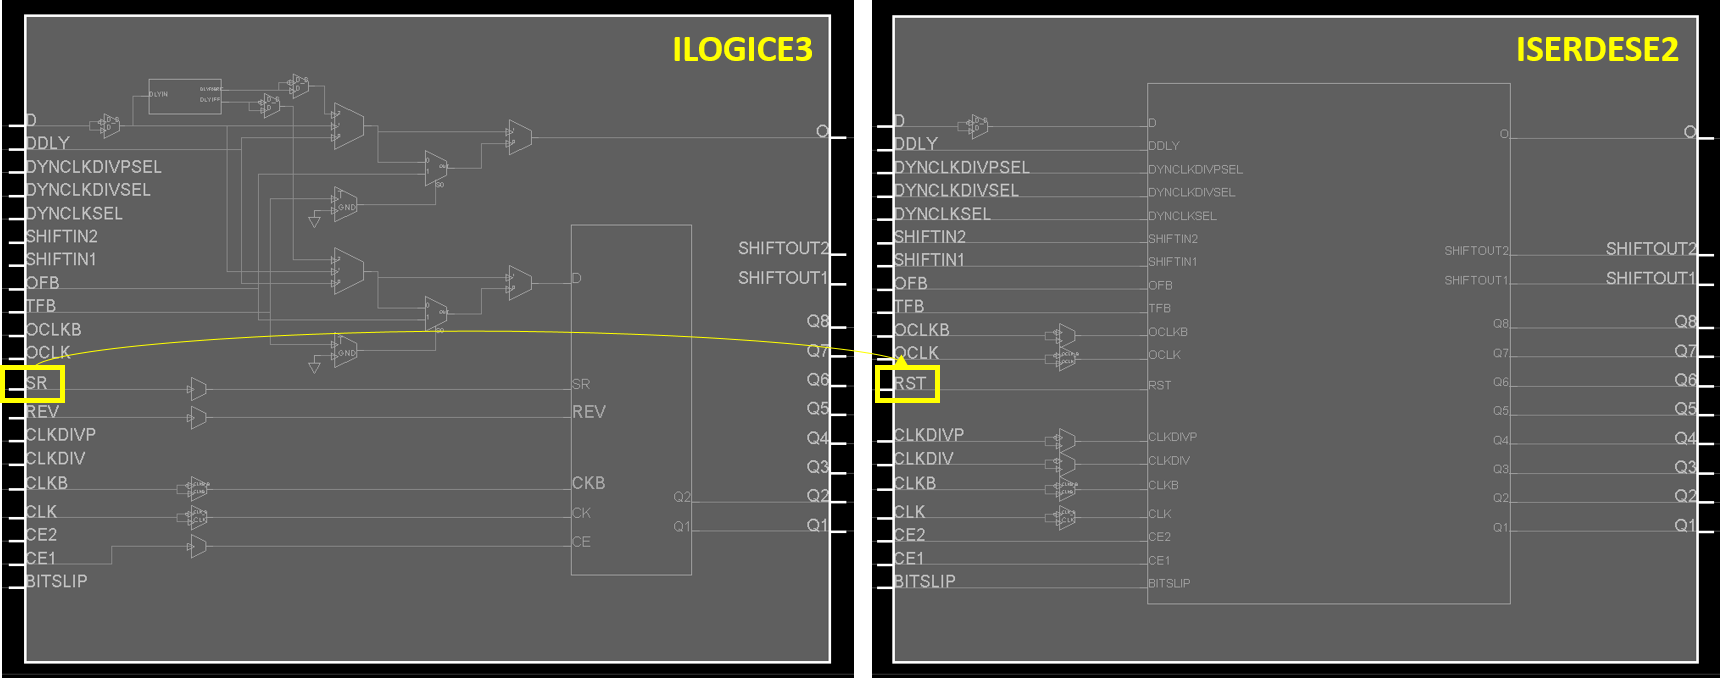
\includegraphics[width=\columnwidth]{alternatePinmap.png}
  \caption{Example Alternate Site Pin Renaming}
  \label{fig:alternatePinmap}
\end{figure}

\begin{enumerate}
\setcounter{enumi}{1}         
      \item  The second hand edit is to add alternate type pin mappings. When a
      site is changed to one of its alternate types in Vivado, the site pins can
      be renamed. An example is shown in \autoref{fig:alternatePinmap} for an
      IDELAYE3 site that has been changed to the alternate type ISERDESE2.
      Notice how the ``SR'' site pin has been renamed to ``RST'' in the figure.
      Unfortunately these pin renamings cannot be automatically extracted from
      Vivado's Tcl interface, and so must be added manually.
      \autoref{lst:apdxAPinmaps} shows how to add pin renamings to the family
      info XML using the ``pinmaps'' tag. To determine the actual pin
      mappings, the first step is to open two instances of the Vivado GUI.
      For each site in the family info, load the default type in one Vivado
      instance, load each alternate type in the other instance, and visibly
      check what pins are renamed in the alternate type (as demonstrated in
      \autoref{fig:alternatePinmap}). \autoref{tab:artix7PinMaps} gives a list
      of all alternate types that rename pins for Artix7 devices.

\end{enumerate}

\begin{lstlisting}[numbers=none, caption=Sample pinmaps in a family info file,
label=lst:apdxAPinmaps] 
      <name>ILOGICE3</name>
      <alternatives>
        <alternative>
          <name>ILOGICE2</name>
          |\textbf{<pinmaps>}|
          |\textbf{</pinmaps>}|
        </alternative>
        <alternative>
          <name>ISERDESE2</name>
          |\textbf{<pinmaps>}|
	        |\textbf{<pin>}|
	          |\textbf{<name>RST</name>}|
	          |\textbf{<map>SR</map>}|
	        |\textbf{</pin>}|
          |\textbf{</pinmaps>}|
        </alternative>
      </alternatives>
\end{lstlisting}
	  
\begin{table} [h!]
    \caption{Artix7 Alternate Pin Mappings}
	\begin{center}
	\begin{tabu}{ |c|c| }
	\hline
	\textbf{Default Type} & \textbf{Alternate Type} \\
	\hline
	\hline 
	FIFO18E1 & RAMB18E1 \\
	\hline
	ILOGICE3 & ISERDESE2 \\
	\hline
	IOB33M & IPAD \\
	\hline
	IOB33S & IPAD \\
	\hline
	OLOGICE3 & OSERDESE2 \\
	\hline
	RAMBFIFO36E1 & FIFO36E1, RAMB36E1 \\
	\hline
	\end{tabu}
	\label{tab:artix7PinMaps}
	\end{center}
\end{table}

\begin{enumerate}
\setcounter{enumi}{2}   	  	  	  
	  \item The third hand edit is to remove invalid mux corrections. In some
	  cases, BELs might be incorrectly tagged as ``routing muxes'' or ``polarity
	  selectors'' even though they are not. This issue has mostly been fixed, but
	  it is still good practice to examine all mux corrections in the
	  family info and verify that they are correct.
	  
	  \item The final hand edit is to add missing compatible types. Some compatible
	  types can be automatically generated from Vivado, but not all. This means
	  that the missing compatible types must be added manually. The next section
	  describes in more detail how to add compatible types to the Family Info XML.
\end{enumerate}

\subsection{UltraScale Family Info Hand Edits} \label{sec:ultrascaleHandEdits}

UltraScale and later devices require only a single hand edit: adding 
missing compatible types (most compatible types can be determined
automatically). The XML listing given in \autoref{lst:apdxACompatibleSites},
shows the two compatible types that were manually added to complete the Kintex
UltraScale family info. Other device families may require additional compatible
site hand edits. It is up to the user to determine what compatible sites need
to be added through experimentation.

\begin{lstlisting}[numbers=none, caption=Manually added compatible sites for
UltraScale devices, label=lst:apdxACompatibleSites] 
    <site_type>
      <name>SLICEL</name>
      <is_slice/>
      |\textbf{<compatible\_types>}|
        |\textbf{<compatible\_type>SLICEM</compatible\_type>}|
      |\textbf{</compatible\_types>}|
      ...
    </site_type>
    <site_type>
      <name>HRIO</name> 
      <is_iob/>
      |\textbf{<compatible\_types>}|
        |\textbf{<compatible\_type>HPIOB</compatible\_type>}|
      |\textbf{</compatible\_types>}|
      ...
    </site_type>
\end{lstlisting}  

%%%%%%%%%%%%%%%%%%%%%%%%%%%%%%%%%%%%%%%%%%%%%%%%%%%%%%%%%%%%%%%%%%%%%%%%%%%%%%%%%%%%%%%%%
% Section 11: Bitstreams in RapidSmith2
%	This section describes how bitstreams are handled in RapidSmith2 (they currently
%   aren't)
%%%%%%%%%%%%%%%%%%%%%%%%%%%%%%%%%%%%%%%%%%%%%%%%%%%%%%%%%%%%%%%%%%%%%%%%%%%%%%%%%%%%%%%%%
\newpage
\section{Bitstreams in RapidSmith2}

In the original RapidSmith, bitstreams can be parsed, manipulated, and exported
for Virtex 4, Virtex 5 and Virtex 6 Xilinx FPGA families.  Because of the
proprietary nature of Xilinx bitstreams, RapidSmith provided only documented
functionality when working with bitstreams (and was limited mainly to
manipulation at the frame level including helping to assemble sequences of
configuration commands which are interpreted by the FPGA configuration
controller circuitry).  While this has proven valuable to many researchers, it
does not provide the ability to create your own bitstream from scratch because
it does not provide the specific meaning of each bit in a bitstream.

If you desire to use RapidSmith's bitstream manipulation features, you should
download and work with RapidSmith instead of RapidSmith2 (the RapidSmith bitstream
packages have been removed from RapidSmith2).  If you do so, note that RapidSmith's
bitstream packages have not been tested beyond Virtex 6.  The authors would be
interested in upgrading RapidSmith's bitstream functionality to device families
beyond Virtex 6 if users create it and are willing to contribute it to us for
inclusion.
%%%%%%%%%%%%%%%%%%%%%%%%%%%%%%%%%%%%%%%%%%%%%%%%%%%%%%%%%%%%%%%%%%%%%%%%%%%%%%%%%%%%%%%%%
% Section 12: License
%	This section contains the license that RapidSmith2 is distributed under
%%%%%%%%%%%%%%%%%%%%%%%%%%%%%%%%%%%%%%%%%%%%%%%%%%%%%%%%%%%%%%%%%%%%%%%%%%%%%%%%%%%%%%%%%
\newpage
\section{License}
RapidSmith2 is released under GPL version 3 with the following license: 

\begin{verbatim}
BYU RapidSmith Tools

Copyright (c) 2010-2016 Brigham Young University
   
BYU RapidSmith Tools is free software: you may redistribute it
and/or modify it under the terms of the GNU General Public License
as published by the Free Software Foundation, either version 2 of
the License, or (at your option) any later version.
   
BYU RapidSmith Tools is distributed in the hope that it will be
useful, but WITHOUT ANY WARRANTY; without even the implied warranty
of MERCHANTABILITY or FITNESS FOR A PARTICULAR PURPOSE. See the GNU
General Public License for more details.
   
A copy of the GNU General Public License is included with the BYU
RapidSmith Tools. It can be found at doc/LICENSE.GPL3.TXT. You may also get
a copy of the license at http://www.gnu.org/licenses/.
\end{verbatim}
%%%%%%%%%%%%%%%%%%%%%%%%%%%%%%%%%%%%%%%%%%%%%%%%%%%%%%%%%%%%%%%%%%%%%%%%%%%%%%%%%%%%%%%%%
% Section 13: Dependency Projects
%	This section contains a list of software dependencies in order to run RapidSmith2.
%	It is important to note that these dependencies are included in the repository
% 	so users don't have to worry about downloading the dependencies themselves.
%%%%%%%%%%%%%%%%%%%%%%%%%%%%%%%%%%%%%%%%%%%%%%%%%%%%%%%%%%%%%%%%%%%%%%%%%%%%%%%%%%%%%%%%%
\newpage
\section{Included Dependency Projects}
RapidSmith2 includes the Caucho Technology Hessian implementation which is distributed
under the Apache License. A copy of this license is included in the
docs/License directory in the file APACHE2-LICENSE.txt. This license is also available for
download at:

\noindent
\hyperref[http://www.apache.org/licenses/LICENSE-2.0]{\color{blue}http://www.apache.org/licenses/LICENSE-2.0}

\bigbreak \noindent
The source for the Caucho Technology Hessian implementation is available at:

\noindent
\hyperref[http://hessian.caucho.com]{\color{blue}http://hessian.caucho.com}

\bigbreak \noindent
RapidSmith2 also includes the Qt Jambi project jars for Windows, Linux and Mac OS X.  Qt
Jambi is distributed under the LGPL GPL3 license and copies of this license and
exception are also available in the docs/License directory in files
LICENSE.GPL3.TXT and LICENSE.LGPL.TXT respectively. These licenses can also be downloaded at:

\noindent
\hyperref[http://www.gnu.org/licenses/licenses.html]{\color{blue}http://www.gnu.org/licenses/licenses.html}

\bigbreak \noindent
Source for the Qt Jambi project is available at:

\noindent
\hyperref[http://qtjambi.org/downloads]{\color{blue}http://qtjambi.org/downloads}, and

\noindent
\hyperref[https://sourceforge.net/projects/qtjambi/files/]{\color{blue}https://sourceforge.net/projects/qtjambi/files/}

\bigbreak \noindent
RapidSmith2 also includes the JOpt Simple option parser which is released under
the open source MIT License which can be found in this directory in the file
MIT\_LICENSE.TXT.  A copy of this license can also be found at:

\noindent
\hyperref[http://www.opensource.org/licenses/mit-license.php]{\color{blue}http://www.opensource.org/licenses/mit-license.php}

\bigbreak \noindent   
A copy of the source for JOpt Simple can also be downloaded at:

\noindent
\hyperref[http://jopt-simple.sourceforge.net/download.html]{\color{blue}http://jopt-simple.sourceforge.net/download.html}

\bigbreak \noindent
RapidSmith2 also includes the JDOM jars.  JDOM is available under an Apache-style open
source license, with the acknowledgment clause removed. This license is among
the least restrictive license available, enabling developers to use JDOM in
creating new products without requiring them to release their own products as
open source. This is the license model used by the Apache Project, which created
the Apache server. The license is available at the top of every source file and
in LICENSE.txt in the root of the JDOM distribution.              

\bigbreak \noindent
The user is responsible for providing copies of these licenses and making
available the source code of these projects when redistributing these jars.

\appendix
%%%%%%%%%%%%%%%%%%%%%%%%%%%%%%%%%%%%%%%%%%%%%%%%%%%%%%%%%%%%%%%%%%%%%%%%%%%%%%%%%%%%%%%%%
% Appendix A: XDLRC Syntax
%	This section provides a detailed description of XDLRC files, and their syntax.
%	Most users of RapidSmith don't need to know the syntax of XDLRC files, but
% 	this information may be useful to new lab members working on the project.
%%%%%%%%%%%%%%%%%%%%%%%%%%%%%%%%%%%%%%%%%%%%%%%%%%%%%%%%%%%%%%%%%%%%%%%%%%%%%%%%%%%%%%%%%
\newpage
\appendix
\section{XDLRC Files and Syntax} \label{sec:appendixXDLRC}
In general, users of RapidSmith do not need to understand the syntax of XDLRC
files to create CAD tools in RapidSmith. The syntax is introduced here for those
who are interested, and for those who want to modify the XDLRC parser
in some way. If these don't apply to you, then go ahead and skip this section.
XDLRC files are textual descriptions of Xilinx FPGA devices and can be very
verbose (which is why they get so large). This section highlights the main parts
of an XDLRC file with accompanying images. As you will see, much of the
terminology is the same as \autoref{fpgaArch}.

\bigbreak \noindent
\begin{large}
\pgm{Tiles}
\end{large}

\begin{figure}[H]
	\centering
	
\includegraphics[width=1\columnwidth]{xdlrcTile}
	\caption{Tile syntax in XDLRC files}
	\label{fig:xdlrcTile}
\end{figure}

\noindent
A tile in an XDLRC file corresponds to the same thing as the \cls{Tile}
described in \autoref{fpgaArch}. Each tile is declared with a ``(tile''
directive as shown above followed by the unique row and column index of where
the tile fits into the grid of tiles found on the FPGA. The tile declaration
also contains a name followed by a type with the final number being the number
of primitive sites found within the tile. The tile ends with a ``tile\_summary''
statement repeating the name and type with some other numbered statistics.
Tiles can contain three different sub components, primitive sites, wires, and
PIPs.

\bigbreak \noindent
\begin{large}
\pgm{Primitive Sites}
\end{large}

\begin{figure}[H]
	\centering
	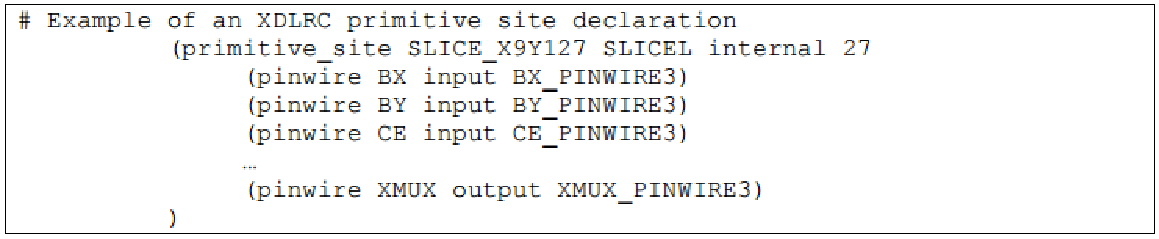
\includegraphics[width=1\columnwidth]{xdlrcSite}
	\caption{Primitive site syntax in XDLRC files}
	\label{fig:xdlrcSite}
\end{figure}

\noindent
Primitive site declarations in XDLRC files contain a list of pinwires which
describe the name and direction of pins on the primitive site. The first
pinwire declared in the example above is the BX input pin which is the internal
name to the SLICEL primitive site. Pinwires have an external name as well to
differentiate the multiple primitive sites that may be present in the same
tile. In this case, BX of SLICE\_X9Y127 has the external name BX\_PINWIRE3. In
RapidSmith, only the first pin name (i.e. BX above) is used.

\bigbreak \noindent
\begin{large}
\pgm{Wire}
\end{large}

\begin{figure}[H]
	\centering
	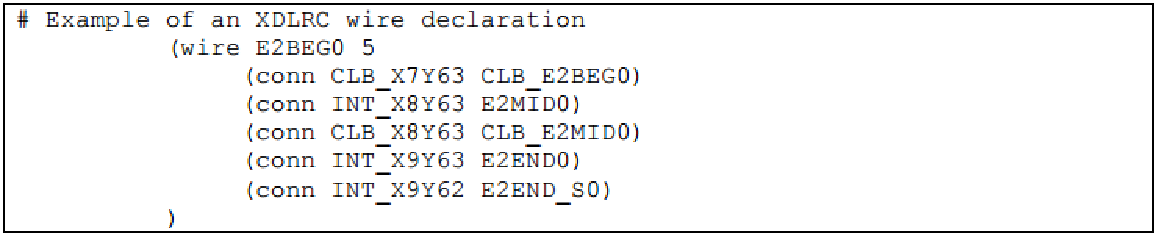
\includegraphics[width=1\columnwidth]{xdlrcWire}
	\caption{Wire syntax in XDLRC files}
	\label{fig:xdlrcWire}
\end{figure}

\noindent
A wire as declared in XDLRC is a routing resource that exists in the tile that
may have zero or more connections leaving the tile. In the example above, the
wire ``E2BEG0'' connects to 5 neighboring tiles. These connections (denoted
by ``conn'') are described using the unique tile name and wire name of that tile
to denote connectivity. The connections are not programmable, but hard wired
into the FPGA. Wire portions of the XDLRC file are included in the definition of
every tile (even if the same tile type has already been printed), which has a
big impact on the final size of XDLRC files. How RapidSmith handles wire
duplication is described in \autoref{wireEnum}. The \cls{WireConnection}
objects that are created from this part of the XDLRC are described in
\autoref{wireConnSection}.

\bigbreak \noindent
\begin{large}
\pgm{PIP}
\end{large}

\begin{figure}[H]
	\centering
	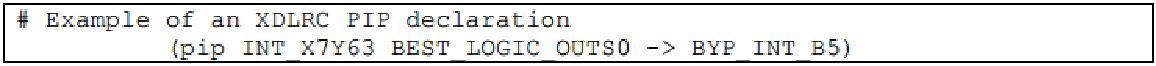
\includegraphics[width=1\columnwidth]{xdlrcPip}
	\caption{PIP syntax in XDLRC files}
	\label{fig:xdlrcPip}
\end{figure}

\noindent
A PIP (programmable interconnect point) is a possible connection that can be
made between two wires. In the example above, the PIP is declared in the tile
and repeats the tile name for reference. It specifies two wires by name that
both exist in that same tile (``BEST\_LOGIC\_OUTS0'' and ``BYP\_INT\_B5'') and
declares that the wire ``BEST\_LOGIC\_OUTS0'' can drive the wire
``BYP\-\_INT\_B5''. A collection of these PIPs in a net define how a net is
routed and is consistent with saying that those PIPs are �turned on.�
\autoref{wireConnSection} describes in detail how PIPs are represented in
RapidSmith.

\bigbreak \noindent
\begin{large}
\pgm{Primitive Definitions}
\end{large}

\bigbreak \noindent
The Primitive Definition portion of an XDLRC file textually describes the
components found within a \cls{Primitive} \cls{Site} (a SLICEL for example)
and how they are connected. This includes: 

\begin{itemize}
  \item BELs
  \item Site Pins 
  \item Site Pips (Routing Muxes) 
  \item Configuration options (both site and BEL)
  \item Site Routethroughs (configurable connections from a site input pin to
  a site output pin)
  \item Site Wire Connections
\end{itemize}

\noindent An example of a complete primitive definition file of type BUFHCE can
be seen in \autoref{fig:xdlrcDef}. The sub-site data structures in RapidSmith
(\cls{Bels}, \cls{SiteWire}s, etc.) are built by parsing this section of the
XDLRC file. For a more detailed description of primitive definitions, view the
VSRT User Guide in the RapidSmith2 repository.

\begin{figure}[H]
	\centering
	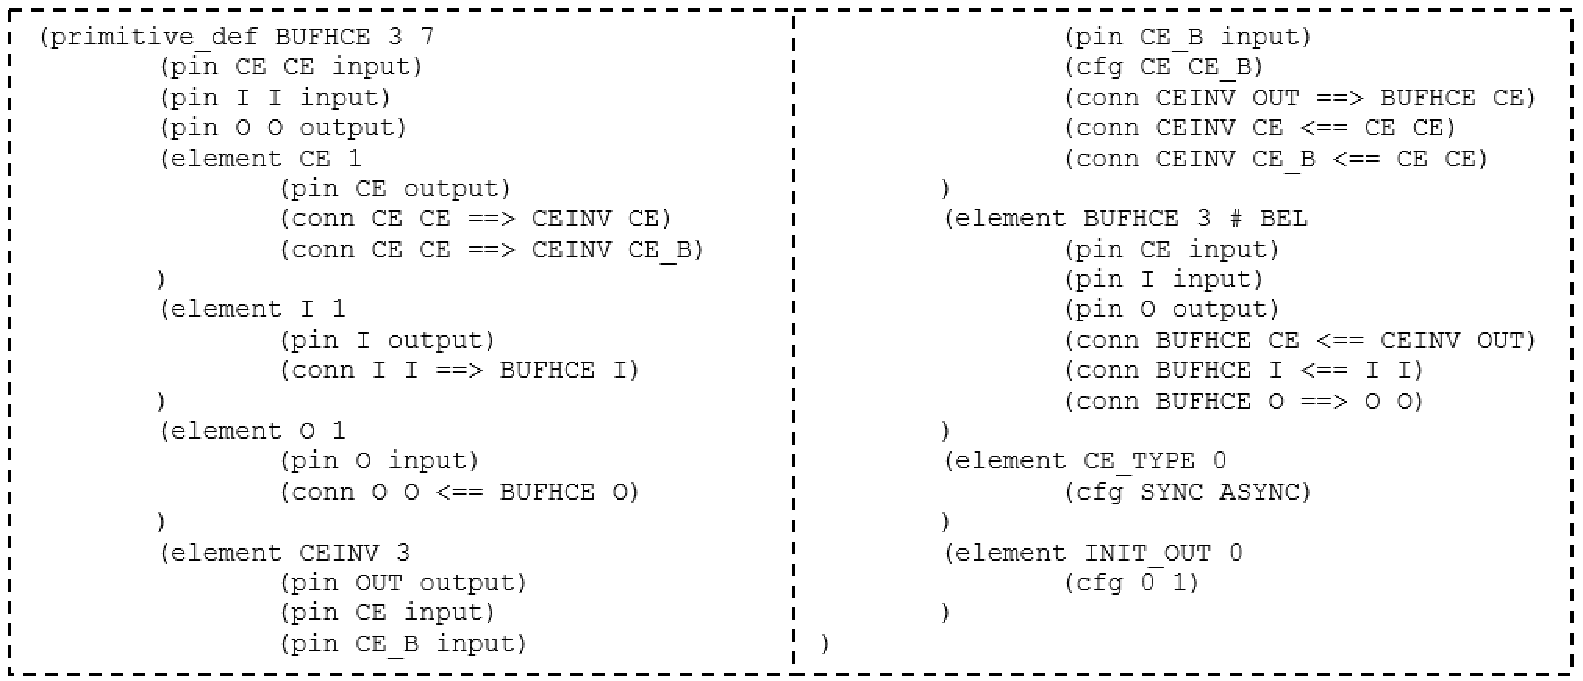
\includegraphics[width=1\columnwidth]{xdlrcDef}
	\caption{Primitive Def sections of XDLRC files}
	\label{fig:xdlrcDef}
\end{figure}
%%%%%%%%%%%%%%%%%%%%%%%%%%%%%%%%%%%%%%%%%%%%%%%%%%%%%%%%%%%%%%%%%%%%%%%%%%%%%%%%%%%%%%%%%
% Appendix B: FamilyInfo XML Files
%	This section provides a detailed description of Family Info files, and their
%   syntax. Most users of RapidSmith2 don't need to know the syntax of family info
%   files, but this information may be useful to new lab members working on the
%   project.
%%%%%%%%%%%%%%%%%%%%%%%%%%%%%%%%%%%%%%%%%%%%%%%%%%%%%%%%%%%%%%%%%%%%%%%%%%%%%%%%%%%%%%%%%
\newpage
\section{Family Info XML} \label{sec:familyInfo}

A \textit{familyInfo.xml} file contains useful information that is
not present in the XDLRC files for a given family of devices. Specifically, it
includes the following additional information about each site type in a family:

\begin{multicols}{2} 
	\begin {itemize}
      \item \textbf{Alternate Types}
      \item \textbf{Compatible Types}
      \item \textbf{BEL Routethroughs}
      \item \textbf{Site PIP Corrections}
      \item \textbf{Pin Direction Corrections}
	\end{itemize}
\end{multicols}

\noindent 
As the name suggests,  only one \textit{familyInfo.xml} is required for each of
the supported Vivado families listed in \autoref{tab:vivadoFamilies} (all
devices within a family share the same family info).  A new \texttt{Tincr}
command has been added to generate family info files:
\texttt{[tincr::create\_xml\_family\_info]}.  Using this command, with a few
required hand edits, \textbf{a complete set of family info XML files have been
created for all Series7 and UltraScale families}.  The following subsections
describe each component of a family info XML and why they may be useful for
external CAD tools.

\subsection{Alternate Types} \label{sec:alternateSites}
Each physical site in a device has an associated default type. Some sites,
however, can be configured to be one of many types (called alternate
types in Vivado). Alternate type information is required for external CAD tools because
the type of a site can be changed during the placement phase of implementation.
To accurately represent a placed design in an external tool, site types need to
be changeable. An example of alternate types for an UltraScale BITSLICE\_RX\_TX
site is shown in \autoref{fig:alternateTypes}. As the figure shows, a
BITSLICE\_RX\_TX site can also be configured to be of type
BITSLICE\_COMPONENT\_RX\_TX, BITSLICE\_RXTX\_RX, or BITSLICE\_RXTX\_TX.
\autoref{lst:familyInfoAlternate} shows how alternate types are
represented in a family info XML. Pinmap tags are included for alternate pin
names changing as decribed in \autoref{sec:series7HandEdits}.

\begin{figure}[b!]
  \centering
  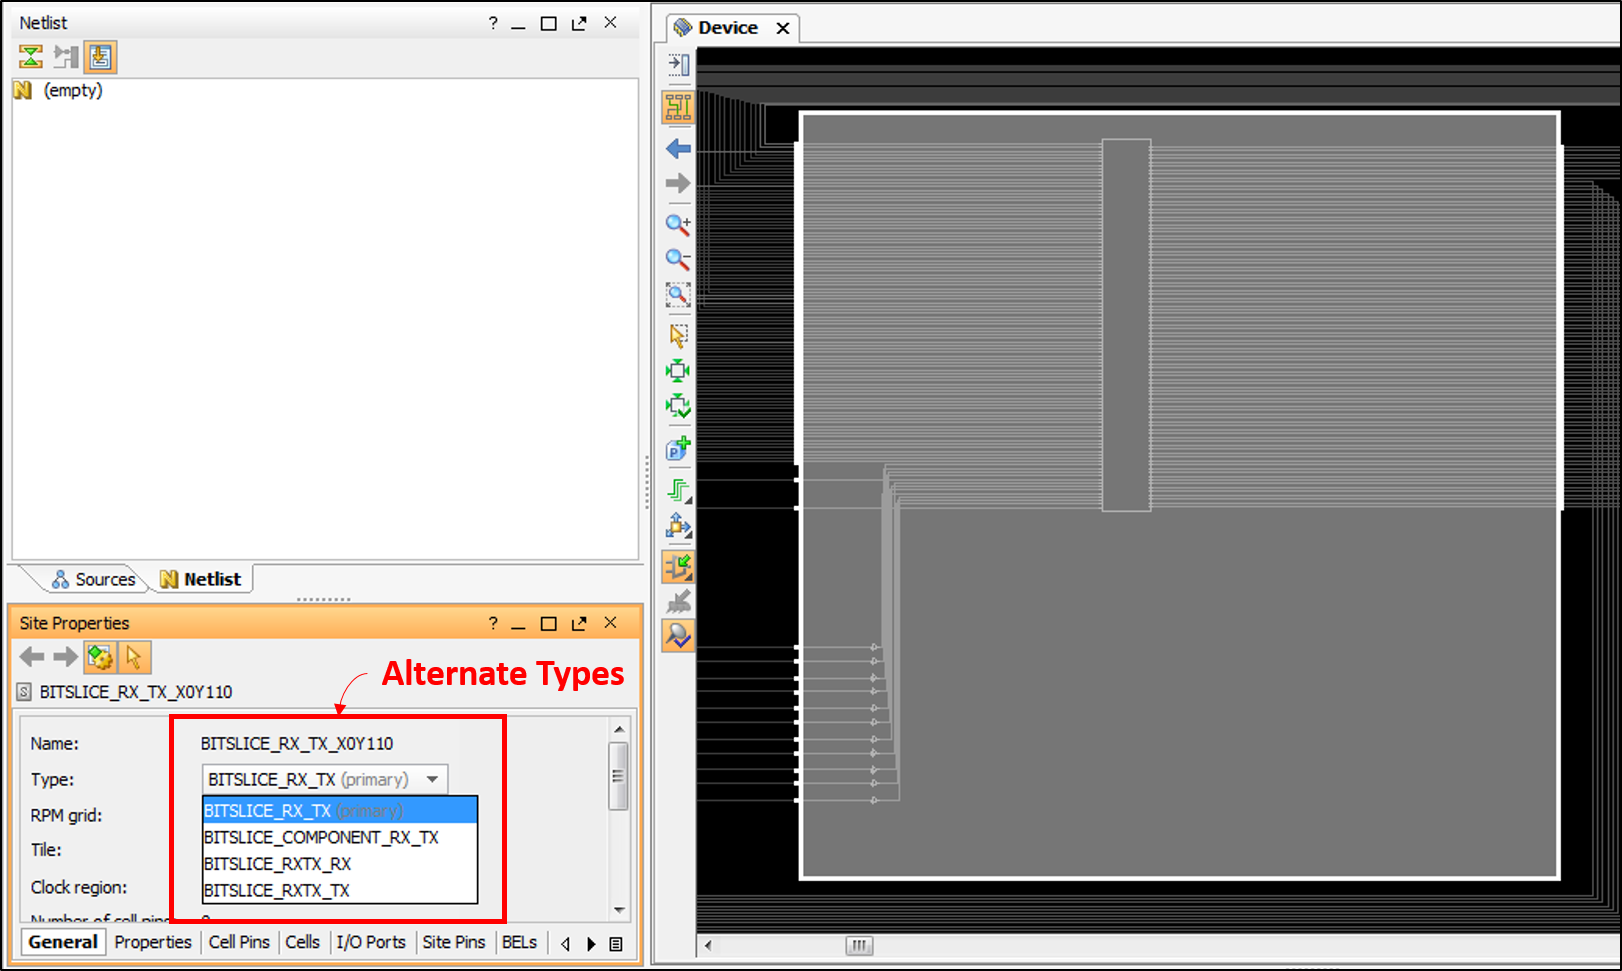
\includegraphics[width=.6\columnwidth]{alternateTypes.png}
  \caption{BITSLICE\_RX\_TX Alternate Types}
  \label{fig:alternateTypes}
\end{figure}

\begin{lstlisting}[numbers=none, keywordstyle=, stringstyle=, caption=Example
Alternate Type XML, label=lst:familyInfoAlternate] 
  <alternative>
      <name>ISERDESE2</name>
      <pinmaps>
          <pin>
	          <name>RST</name>
              <map>SR</map>
	      </pin>
      </pinmaps>
  </alternative>
\end{lstlisting}

\subsection{Compatible Types}
Site \texttt{A} is said to be compatible with site \texttt{B} if the logical
cells placed on site \texttt{A} can \textit{always} be placed on site \texttt{B}
as well. For example, as shown in \autoref{fig:sliceCompatibility}, SLICEL sites
are compatible with SLICEM sites. The cells placed on the SLICEL in the figure
can be moved to the SLICEM and still function identically. SLICEMs, however,
are \textit{not} compatible with SLICELs. This is because SLICEM sites support
LUT RAM cells, which cannot be placed on SLICEL sites.  In some cases of
compatibility, the type of the compatible site must first be changed before
placing cells on it. For instance, a RAMB36 site is compatible with a
RAMBFIFO36 site, but the site type of the RAMBFIFO36 \textbf{must
first be changed to RAMB36} before it is truly compatible. 

\begin{figure}[h!]
  \centering
  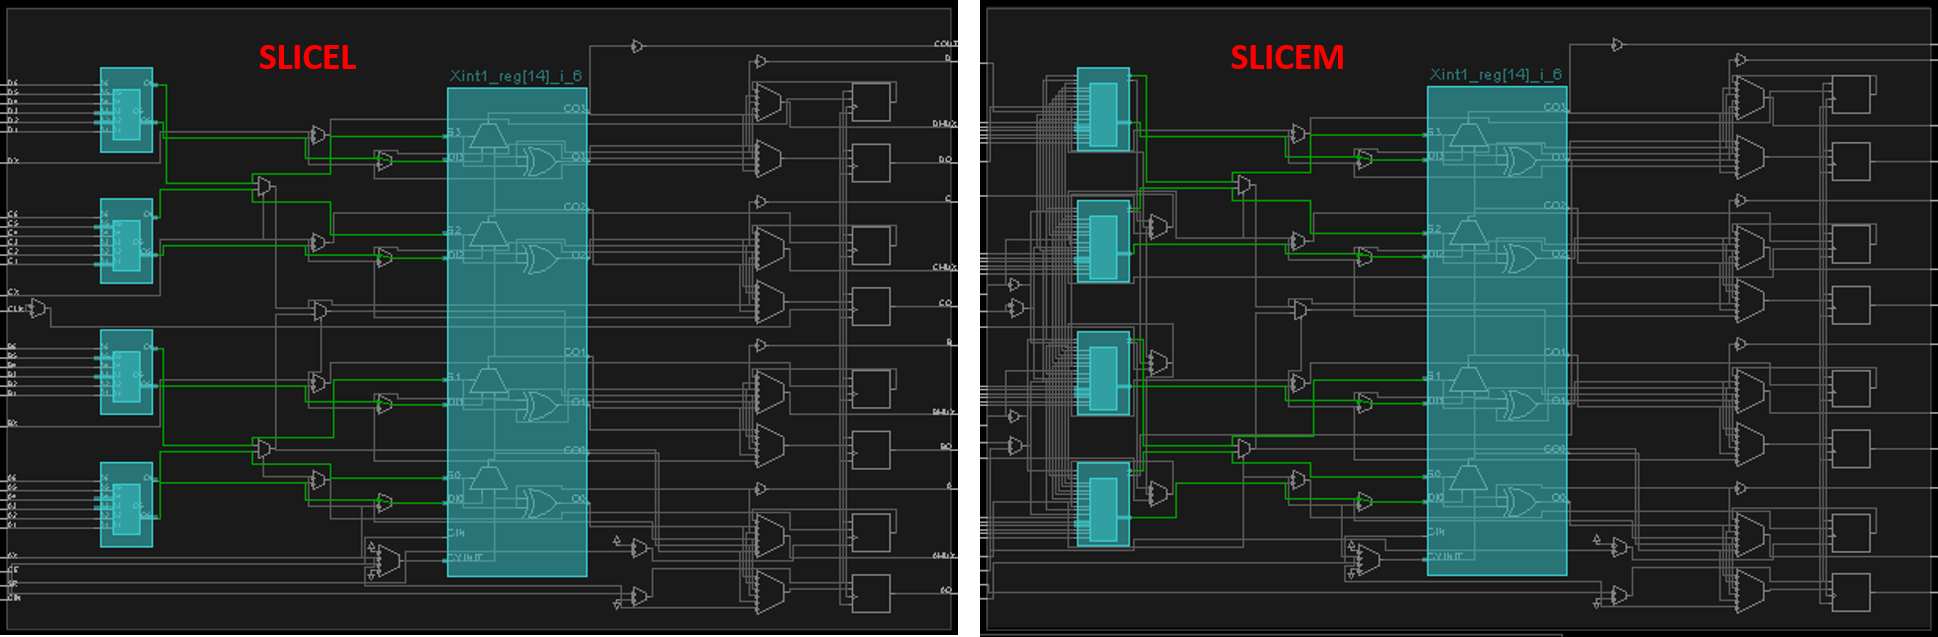
\includegraphics[width=1\columnwidth]{compatibleSites.png}
  \caption{A group of cells placed on a SLICEL site (left) and a SLICEM
  site (right).}
  \label{fig:sliceCompatibility}
\end{figure}

\begin{figure}[b!]
  \centering
  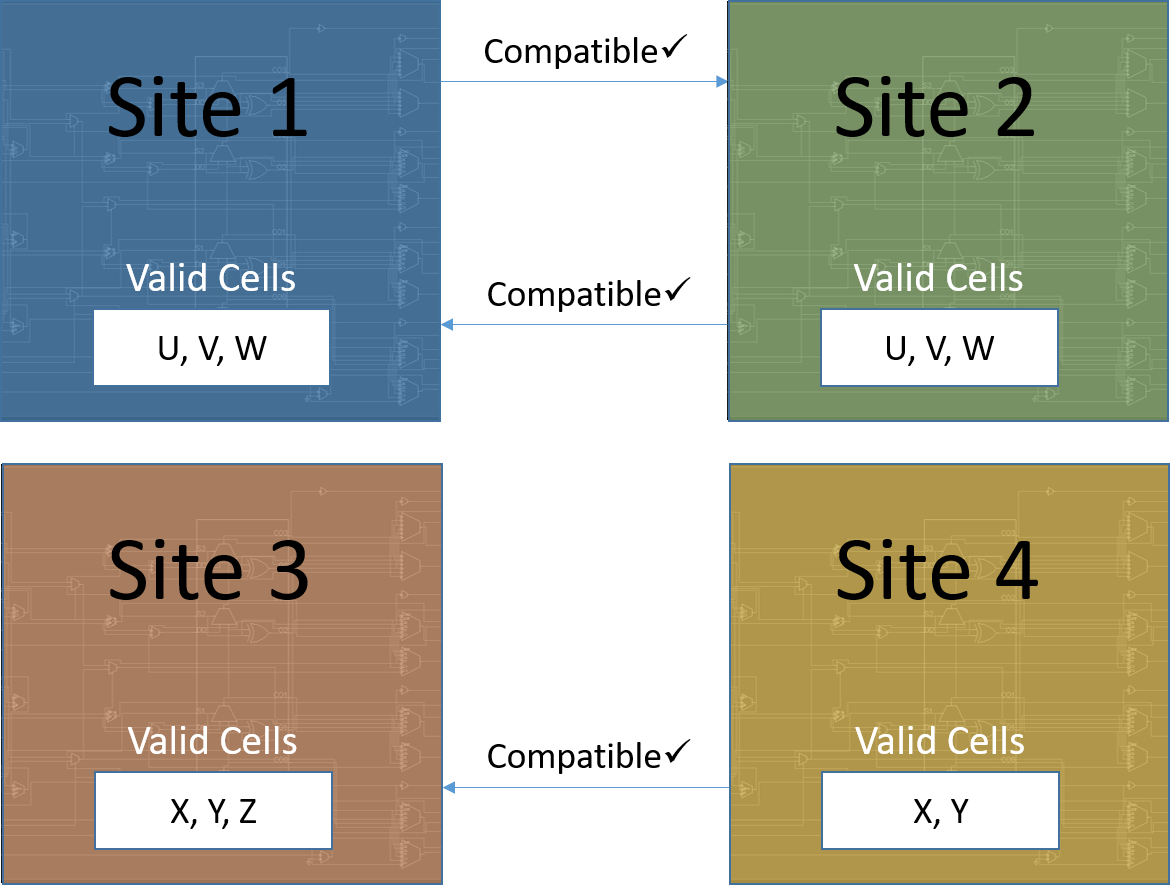
\includegraphics[width=.6\columnwidth]{compatibleTest.png}
  \caption{Compatibility Testing for Single-BEL Sites}
  \label{fig:singleBelCompatibleTest}
\end{figure}

A visualization of compatibility is also given in
\autoref{fig:singleBelCompatibleTest}. In this case, ``Site 1'' and ``Site 2''
are both compatible to each other since the same set of cells can be placed
onto both sites. ``Site 4'' is compatible with ``Site 3'' because each cell that
can be placed on ``Site 4'' can also be placed on ``Site 3.'' ``Site 3'', however, is
not compatible with ``Site 4'' because cell \texttt{Z} cannot be placed on
``Site 4.''

Information about compatible types is useful in a variety of CAD applications.
One such application is a site-level placer. To achieve the best
placement results, the placer needs to understand \emph{all} available
locations where a set of cells can be placed. Without information about
compatible types, the placer would only know how to target one specific site
type for each group of cells, lowering the quality of results.
\autoref{lst:compatibleTypes} shows example XML for compatible types in a
family info file.

\begin{lstlisting}[numbers=none, keywordstyle=, stringstyle=,
caption=Compatible Type XML for SLICEL, label=lst:compatibleTypes]
  <compatible_types>
    <compatible_type>SLICEM</compatible_type>
  </compatible_types>
\end{lstlisting}

\subsection{BEL Routethroughs}
During the routing stage of implementation, certain BELs can be configured as
PIPs in a device (i.e. they pass a signal from an input pin directly to an
output pin). To fully represent the routing structure within
a Xilinx FPGA, these \textbf{routethrough} connections are included in the
family info file. \autoref{lst:familyInfoRoutethrough} shows how routethrough
connections are represented. External tools can use this information to
build a more accurate device data structure. At the time of writing, BELs are
considered routethrough candidates if they are of type ``LUT" or ``Flip-Flop"
on a SLICE site. A more detailed discussion of routethroughs is presented in
\autoref{sec:belRoutethroughs}.

\begin{lstlisting}[numbers=none, keywordstyle=, stringstyle=,
caption=Example Routethrough XML, label=lst:familyInfoRoutethrough]
  <bel>
      <name>D6LUT</name>
      <type>LUT6</type>
      <routethroughs>
          <routethrough>
              <input>A1</input>
              <output>O6</output>
          </routethrough>
          <routethrough>
              <input>A2</input>
              <output>O6</output>
          </routethrough>
      <routethroughs>
  </bel>
\end{lstlisting}

\subsection{Site PIP Corrections}
XDLRC files do not distinguish the difference between site PIPs (routing muxes)
and functional BELs within a site. Each of these components are simply marked
as a ``Bel'', even though site PIPs are certainly not BELs. The family info file
corrects this by explicitly marking site PIPs as \textbf{routing muxes} or
\textbf{polarity selectors}. A polarity selector is a site PIP with one
input that can be optionally inverted. \autoref{lst:pipCorrectionXml} shows how
site PIP corrections are represented in a family info file.

\begin{lstlisting}[numbers=none, keywordstyle=, stringstyle=,
caption=Example Site PIP Corrections, label=lst:pipCorrectionXml]
  <corrections>
      <modify_element> 
          <name>A5FFMUX</name> 
          <type>mux</type> 
      </modify_element>
      <polarity_selector> 
          <name>CLKINV</name> 
      </polarity_selector>
  </corrections>
\end{lstlisting}

\noindent RapidSmith2 decomposes a site PIP into its individual PIPs as shown in
\autoref{fig:sitePipDecomposition}. This decomposition generally makes creating
routing algorithms easier. In Vivado, site PIPs are determined with the Tcl
command \texttt{[get\_site\_pips -of \$site]}. Polarity selectors are
distinguished from regular site PIPs by checking if the string name of the PIP
ends with either ``INV'' or ``OPTINV''.
  
\begin{figure}[H]
  \centering
  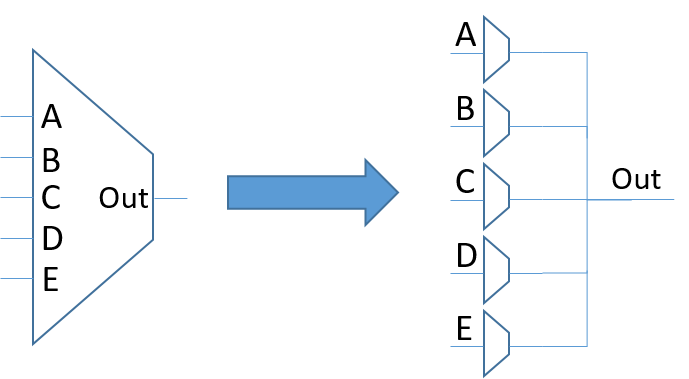
\includegraphics[width=.6\columnwidth]{sitePipDecomposition.png}
  \caption{Site PIP Decomposition}
  \label{fig:sitePipDecomposition}
\end{figure}

\subsection{Pin Direction Corrections}
In XDLRC files, all BEL pins are given a direction of either INPUT or OUTPUT.
However, there are several BEL pins in Xilinx devices that are of direction
INOUT (bidirectional). The family info file marks INOUT BEL pins so that their
direction can be corrected in RapidSmith2. The direction of a BEL pin in
Vivado can be determined with the Tcl command \texttt{[get\_property DIRECTION
\$belpin]}. \autoref{lst:pindirCorrectionXml} shows how pin direction
corrections are represented in XML.

\begin{lstlisting}[numbers=none, keywordstyle=, stringstyle=,
caption=Example Pin Direction Correction, label=lst:pindirCorrectionXml]
  <corrections>
      <pin_direction>
          <element>PAD</element>
          <pin>PAD</pin>
          <direction>inout</direction>
      </pin_direction>
  </corrections>
\end{lstlisting}
%%%%%%%%%%%%%%%%%%%%%%%%%%%%%%%%%%%%%%%%%%%%%%%%%%%%%%%%%%%%%%%%%%%%%%%%%%%%%%%%%%%%%%%%%
% Appendix C: DeviceInfo XML Files
%	This section provides a detailed description of Family Info files, and their
%   syntax. Most users of RapidSmith2 don't need to know the syntax of family info
%   files, but this information may be useful to new lab members working on the
%   project.
%%%%%%%%%%%%%%%%%%%%%%%%%%%%%%%%%%%%%%%%%%%%%%%%%%%%%%%%%%%%%%%%%%%%%%%%%%%%%%%%%%%%%%%%%
\newpage
\section{DeviceInfo Info XML} \label{sec:deviceInfo}
A device info XML file contains additional information \textbf{specific to a
device} that is not found in the corresponding XDLRC for the device. Currently,
the device info file contains only a list of package pins for the device as
shown in \autoref{lst:deviceInfoXml}. Each package pin definition has three
attributes:

\begin{enumerate}
  \item \textbf{The name of the package pin}: Generally, package pin names are a
  single letter followed by a two-digit number (i.e. M17). For those that have
  written UCF or XDC constraints for a FPGA design targeting a Xilinx part, this
  format should be familiar.
  \item \textbf{The corresponding PAD BEL for the package pin}: Each
  package pin maps to a specific BEL in the device. Both the name of the
  BEL as well as its parent site is recorded in the form ``site/belname.''
  \item \textbf{An optional ``is\_clock'' attribute}: Only a select number of
  package pins in a device can access the global clock routing resources. These
  package pins are explicitly marked in the device info file so external CAD
  tools can use this information when placing clock ports (or other signals
  that need access to global routing).
\end{enumerate}

\noindent Device info files can be generated with the \texttt{Tincr}
command \texttt{[tincr::create\_xml\_device\-\_info]}. This command is fully
automated, and requires no hand edits.

\begin{lstlisting}[numbers=none, keywordstyle=, stringstyle=,
caption=Example Device Info XML, label=lst:deviceInfoXml]
  <device_info>
      <partname>xcku025-ffva1156</partname>
      <package_pins>
          <package_pin>
              <name>AK33</name>
              <bel>IOB_X0Y155/PAD</bel>
          </package_pin>
          <package_pin>
              <name>AJ29</name>
              <bel>IOB_X0Y130/PAD</bel>
              <is_clock/>
          </package_pin>
          ...
      </package_pins>
  </device_info>
\end{lstlisting}

%%%%%%%%%%%%%%%%%%%%%%%%%%%%%%%%%%%%%%%%%%%%%%%%%%%%%%%%%%%%%%%%%%%%%%%%%%%%%%%%%%%%%%%%%
% Appendix D: RapidSmith Checkpoints 
%	This section provides a overview of the contents of a RapidSmith Checkpoint
%   (RSCP). A very detailed description of TCPs is given in Thomas Townsend's 
%   Masters thesis available at http://scholarsarchive.byu.edu/etd/6492/
%%%%%%%%%%%%%%%%%%%%%%%%%%%%%%%%%%%%%%%%%%%%%%%%%%%%%%%%%%%%%%%%%%%%%%%%%%%%%%%%%%%%%%%%%
\newpage
\section{VDI Checkpoint Formats} \label{sec:rscpTcp}
\graphicspath{{./techReportFigures/appendixD/} {./techReportFigures/sec5_designs/}}

Before reading this appendix, it is encouraged for the reader to first read
Thomas Townsend's master thesis located for download at: {\color{blue}
http://scholarsarchive.byu.edu/etd/6492/}. This document gives a very detailed
introduction to the \textbf{Vivado Design Interface}, the interface used to
extract device and design information out of Vivado. 

\vspace{.3cm}

Vivado Tcl commands are used to define an alternate checkpoint representation
for open-source tools. VDI defines two different external design
representations:

\begin{enumerate}
  \item \textbf{RapidSmith Checkpoints (RSCP)}: Represents designs that have
  just been exported from Vivado. These checkpoints are intended to be loaded
  into external tools.
  \item \textbf{Tincr Checkpoints (TCP)}: Represents designs
  that can be loaded back into Vivado.
\end{enumerate}

\noindent Each of these checkpoints are capable of representing a Vivado design
post-synthesis, post-place, and post-route, enabling the design flows shown 
\autoref{fig:vdiDesign}. The remainder of this chapter describes each external
design representation, and the required Tcl commands to generate each.
Section \ref{sec:vdiImport} introduces RSCPs and Section~\ref{sec:vdiExport} introduces
TCPs. Section \ref{sec:tclChallenges} lists the variety of Tcl challenges
associated with using the Vivado Tcl interface to represent designs externally.
Section \ref{sec:twoFormats} includes a discussion on why two different external
design formats are necessary. The purpose of this appendix is to document the
format of RSCPs and TCPs so that maintainers of RapidSmith2 will understand how
to parse/generate these files. These checkpoint formats may change with future
versions of Vivado. \textbf{General users of RapidSmith2 can ignore this
appendix}.

\begin{figure}[h!]
  \centering
  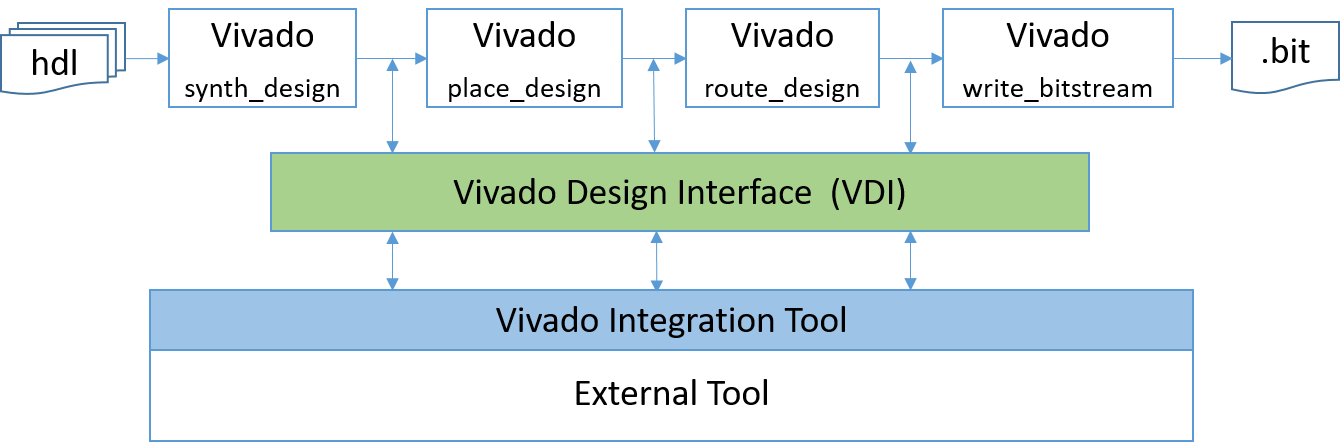
\includegraphics[width=.9\columnwidth]{vdiDesign.png}
  \caption{Vivado Design Interface (VDI) Design Flows}
  \label{fig:vdiDesign}
\end{figure}

%%%%%%%%%%%%%%%%%%%%%%%%%%%%%%%%%%%%%
%			RSCPs
%%%%%%%%%%%%%%%%%%%%%%%%%%%%%%%%%%%%%
\subsection{Design Export (RSCP Format)} \label{sec:vdiImport}
% TODO: mention that an RSCP can represent a Vivado design post synth, place or
% route.
VDI exports Vivado FPGA designs in the form of \textbf{RapidSmith Checkpoints}
(RSCP). A RSCP is a fileset containing 6 individual files: 

% Have a individual section for each of these and then discuss the Vivado Tcl
% challenged individually
\begin{multicols}{2}
	\begin {itemize}
	  \item design.info
	  \item netlist.edf
	  \item macros.xml
	  \item contraints.xdc
	  \item placement.rsc
	  \item routing.rsc
	\end{itemize}
\end{multicols}

\noindent Each file represents a specific aspect of a Vivado FPGA design, and
is described in the following subsections. The new \texttt{Tincr} command
\texttt{[tincr::write\_rscp]} can generate valid RSCPs for
\textbf{fully-flattened} Vivado designs. It is important to note that the name
``RapidSmith'' does not make the checkpoints exclusive to RapidSmith. The name
was arbitrarily chosen to match the external CAD framework used to test and
validate VDI. Any external tool that desires to operate on Vivado designs can
use these checkpoints.

\subsubsection{Design.info}
The \textit{design.info} file of a RSCP is reserved for additional information
about a design that is not related to the design netlist or implementation. It
currently only holds two pieces of information: (1) the part name that the
design is implemented on, and (2) the checkpoint ``mode''. The part name is
technically redundant, in that it is also included in the EDIF netlist
(described in the next subsection), but can be easier to parse than its EDIF equivalent. The
checkpoint mode refers to the type of checkpoint that was exported from Vivado.
If the Vivado design was implemented out-of-context, then the mode value will
be \texttt{out\_of\_context}. Otherwise, the mode value will be
\texttt{regular}. Because out-of-context checkpoints do not route to
peripheral FPGA pins, external tools or frameworks that parse RSCPs may need to
handle out-of-context designs differently. \autoref{lst:designInfo} shows an
example \textit{design.info} file. 

\begin{lstlisting}[numbers=none, keywordstyle=, stringstyle=, caption=
Sample design.info, label=lst:designInfo]
  part=xc7a100tcsg324-3
  mode=out_of_context	
\end{lstlisting}

\subsubsection{Netlist.edf}
The \textit{netlist.edf} file within a RSCP is an EDIF netlist representing the
logical portion of a design. It details all cells, nets, and
top-level ports within a design, and is generated from Vivado using the Tcl
command \texttt{[write\_edif]}. An example EDIF file is shown
\autoref{lst:edif}. External tools can use any open-source EDIF parser (such as
BYU EDIF tools) to translate the EDIF into their own design representation to
perform netlist modifications.

\begin{lstlisting}[numbers=none, keywordstyle=, stringstyle=, caption=
Sample EDIF, label=lst:edif]
  (Library work
    (edifLevel 0)
    (technology (numberDefinition ))
    (cell add (celltype GENERIC)
      (view add (viewtype NETLIST)
        (interface
          (port a (direction INPUT))
          (port b (direction INPUT))
          ...
        )
        (contents
          (instance cout_OBUF (viewref netlist (cellref OBUF (lib hdi_primitives))))
          (instance cout_lUT (viewref netlist (cellref LUT3 (libref hdi_primitives))) 
            (property INIT (string "8'hE8"))
          )
          ...	
\end{lstlisting}

\subsubsection{Constraints.xdc}
The \textit{constraints.xdc} file within a RSCP stores all user-defined XDC
constraints on a Vivado design. XDC constraint files are similar to UCF files
for ISE designs. Constraints can be used to set the clock frequency, constrain
a top-level port to a specific package pin on the device, and set other
physical implementation details. An example RSCP constraints file can be
seen in \autoref{lst:constraintsRsc}, and is essentially a list of Tcl commands.

\begin{lstlisting}[numbers=none, keywordstyle=, stringstyle=, caption=
Sample constraints.xdc, label=lst:constraintsRsc]
  create_clock -period 5.000 -name sysClk -waveform {0.000 2.500}
  set_property IOSTANDARD LVCMOS18 [get_ports clk]
  set_property IOSTANDARD LVCMOS18 [get_ports ena]
  set_property PACKAGE_PIN E15 [get_ports {Yin[12]}]
  set_property PACKAGE_PIN H17 [get_ports {Xin[14]}]
  set_property PACKAGE_PIN D18 [get_ports {Xin[7]}]
\end{lstlisting}

\subsubsection{Macros.xml} \label{sec:macrosRscp}

%  that had been flattened during synthesis
Many fully-flattened Vivado designs contain \textbf{hidden macros}. Hidden
macros are Vivado macro primitives that are not returned from the Tcl command
\texttt{[get\_lib\_cells]}, but are used in a netlist anyway. For example, the
macro primitive IOBUF is found in a variety of Series7 designs, but
the Vivado Tcl command \texttt{[get\_lib\_cells IOBUF]} returns an empty string
indicating that the library cell cannot be found. This breaks the well defined
assumption that \texttt{[get\_lib\_cells]} returns a list of \textit{all}
Xilinx primitives that can be used in a design netlist. Hidden macros create two
problems in particular:

\begin{enumerate}
  \item Because \texttt{[get\_lib\_cells]} is used to generate the cell library
   XML, the default cell library XML returned from
   \texttt{[tincr::create\_xml\_cell\_library]} is incomplete and only supports
   the subset of designs without hidden macros.
   \item Hidden macros are ``primitive" cells in Vivado's perspective.
   Therefore, the internal structure of hidden macros is not expanded in the
   \textit{netlist.edf} file described above. They are simply black box cells to
   external tools
\end{enumerate}

RSCPs handle hidden macros by including a \textit{macros.xml} file
which contains template information about each hidden macro in a Vivado design.
This file has the same format as regular cell library macros as shown in
\autoref{lst:macroXml}. External tools can augment their default cell library with
the cells found in \textit{macros.xml} to create a complete list of
primitives used in a given design. An alternative approach is to include
placement information for the macro. 

%VDI does not currently support relatively placed macros (RPM), making
%it difficult to fully represent Vivado designs using only a cell library and
%EDIF netlist. 

\subsubsection{Placement.rsc}

% TODO: add information about internal properties here

The \textit{placement.rsc} file within a RSCP stores all the placement
information of a Vivado design. Specifically, the file includes four different
tokens to differentiate placement data:

\begin{itemize}
  \item \textbf{LOC}: Gives the site and BEL that a cell in the
  netlist is placed on. An example is shown on line 3 of
  \autoref{lst:placementRsc}. In this case, the cell named
  ``cout\_OBUF\_inst\_i\_1'' is placed onto the ``A6LUT'' BEL of the
  ``SLICE\_X0Y51'' site. The site type (SLICEL) is also given after the site
  name in case the site needs to be changed to an alternate type before
  placing the cell (not required for the example cell placement). 
  
  \item \textbf{PINMAP}: Gives the logical-to-physical mapping for each cell
  pin attached to a given cell. Line 4 of \autoref{lst:placementRsc} shows the
  cell pin mappings for ``cout\_OBUF\_inst\_i\_1.'' As can be seen, the
  ``O'' cell pin is mapped to the ``O6'' BEL pin of the A6LUT, the I0 cell pin
  is mapped to the A4 BEL pin, etc. These pin mappings are required in
  \textit{placement.rsc} because certain cells can have different pin mappings
  based on how they are configured.  For example, the pin mappings for a BRAM
  cell with a data width of 72 bits differ from the pin mappings of the same
  BRAM cell with a data width of 9 bits, even if they are placed at the same
  physical location. \texttt{PINMAP} tokens help external tools guarantee
  that the pin mappings for each cell are correct. Cell pin mappings
  contained in the cell library are for the cell's \textbf{default
  configuration} only. Future work includes creating a more detailed pin
  mapping in the cell library so that the \texttt{PINMAP} token is no longer
  required in \textit{placement.rsc}.
  
  \item \textbf{PACKAGE\_PIN}: Gives the site and BEL that a top-level port
  is mapped to. Line 6 of \autoref{lst:placementRsc} shows an example for a port
  named ``fsync\_out.'' In this case, ``fsync\_out'' is mapped to the ``PAD'' BEL on
  the ``IOB\_X1Y30'' site.
  
  \item \textbf{IPROP}: Gives the value of an internal cell property (to a
  macro). Internal cell properties are not included within in the EDIF
  netlist, and so are included in \textit{placement.rsc} for completeness. 
\end{itemize}

\noindent If a design has not yet been placed, \textit{placement.rsc} will be
empty. It is important to note that for macro primitives in a design, only the
placement information for internal cells to the macro are included.
\autoref{lst:placementRsc} demonstrates the order in which the above tokens
appear in the file. \autoref{fig:cellPlacement} shows a visual representation
of how cells are placed onto BELs in Vivado.

\begin{lstlisting}[xleftmargin=1.5em, framexleftmargin=1.5em, keywordstyle=,
stringstyle=, caption= Sample placement.rsc, label=lst:placementRsc]
	IPROP seq_ram_reg_0_127_0_0/DP.HIGH INIT 64'h0000000000000000
	...
	LOC a_IBUF_inst R10 IOB33 INBUF_EN
	PINMAP a_IBUF_inst O:OUT I:PAD
	LOC cout_OBUF_inst_i_1 SLICE_X0Y51 SLICEL A6LUT
	PINMAP cout_OBUF_inst_i_1 O:O6 I0:A4 I1:A5 I2:A6
	...
	PACKAGE_PIN fsync_out IOB_X1Y30 PAD
	PACKAGE_PIN data_out[7] IOB_X1Y33 PAD
	...  
\end{lstlisting}

\begin{figure}[h!]
  \centering
  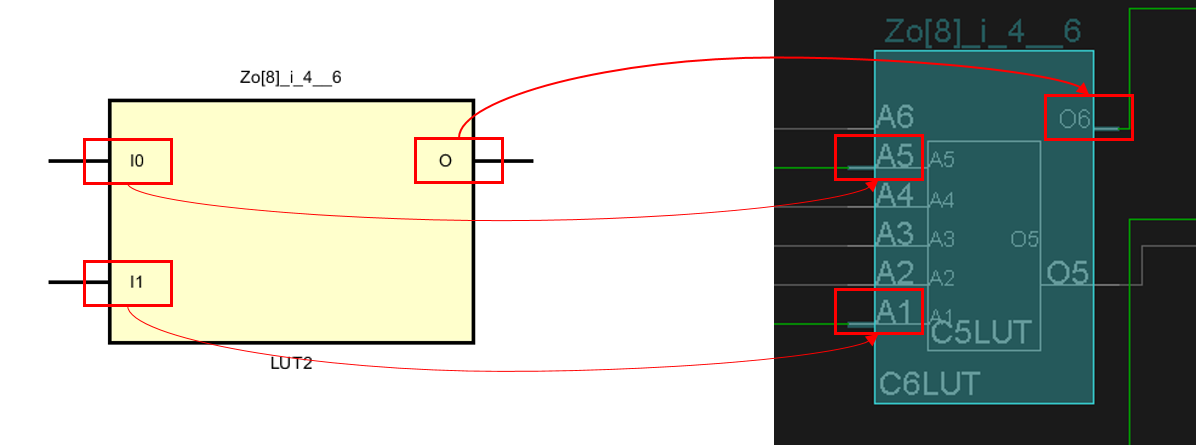
\includegraphics[width=\columnwidth]{cellPlacement.png}
  \caption{Example Cell Placement}
  \label{fig:cellPlacement}
\end{figure}

\subsubsection{Routing.rsc} \label{sec:routingRsc}

The \textit{routing.rsc} file is the most complex file of a RSCP, and stores a
complete description of all routing resources used in a Vivado design.
Specifically, it contains the following:

\begin{itemize}
  \item The intrasite routing configuration for each site in the form of
  used site PIPs (routing muxes)
  \item A list of BELs configured as routethroughs (both LUT and flip-flops).
  %This includes the input pin, output pin, and BEL of each routethrough.
  \item A list of BELs configured as static VCC/GND sources. 
  \item \textbf{Intrasite} nets.
  \item Routed \textbf{intersite} nets with their corresponding site pins and
  used PIPs.
  \item The \textbf{merged} physical routing information for VCC and GND nets.
\end{itemize}


\noindent An example \textit{routing.rsc} is shown in \autoref{lst:routingRsc}.
If a design has not yet been routed, only the intrasite routing information will be
included in this file. If the design has not yet been placed, this file will be
empty. The rest of this section describes each component within a
\textit{routing.rsc} file, and how they can be determined in Vivado.

\begin{lstlisting}[xleftmargin=1.5em, framexleftmargin=1.5em, keywordstyle=,
stringstyle=, caption= Sample routing.rsc, label=lst:routingRsc]
	SITE_PIPS SLICE_X9Y80 SRUSEDMUX:0 CEUSEDMUX:IN CLKINV:CLK  ...
	SITE_PIPS SLICE_X13Y80 PRECYINIT:AX SRUSEDMUX:0 COUTUSED:0 ...
	...
	VCC_SOURCES SLICE_X5Y104/C6LUT/O6 SLICE_X5Y102/C6LUT/O6 ...
	GND_SOURCES SLICE_X2Y106/D6LUT/O6 SLICE_X2Y106/C6LUT/O6 ...
	LUT_RTS SLICE_X5Y101/B6LUT/A6/O6 SLICE_X40Y96/DFF/D/Q  ...
	...
	INTRASITE AddSub[10]
	INTERSITE AngStep1[0] SLICE_X2Y82/AX SLICE_X2Y87/AQ SLICE_X2Y84/A1 ... 
	ROUTE AngStep1[0] INT_X28Y26/INT.LOGIC_OUTS_W1->>SDNDSW_W_0_FTS ...
	...
	VCC INT_L_X2Y107/INT_L.VCC_WIRE->>IMUX_L42 ...
	START_WIRES INT_L_X2Y107/VCC_WIRE INT_L_X2Y106/VCC_WIRE ...
	GND INT_R_X3Y106/INT_R.GND_WIRE->>GFAN1 ...
	START_WIRES INT_R_X3Y106/GND_WIRE INT_L_X4Y106/GND_WIRE ...
\end{lstlisting}

\subsubsection{Site PIPs}

The internal routing structure of nets inside Vivado sites are represented by
a set of used site PIPs. A string of site PIPs enables a connection between site
components. An example is shown in \autoref{fig:sitePips2} where the used site
PIPs are circled in red. As can be seen, the \texttt{ACY0:05} site PIP is
enabled and connects the \texttt{05} pin of the \texttt{A5LUT} BEL to the
\texttt{DI0} pin of the \texttt{CARRY4} BEL. Site PIPs can also be used to 
connect site pins to BEL pins. The Vivado Tcl command \texttt{[get\_site\_pips -of \$site -filter
IS\_USED]} can be used to obtain a list of used site PIPs within a given site.
\texttt{[tincr::write\_rscp]} formats the site pips as shown on line 1 and 2 of
\autoref{lst:routingRsc}. External tools can use the \texttt{SITE\_PIPS} token
within a \textit{routing.rsc} file to reconstruct the internal routing of
each site.

\begin{figure}[h!]
  \centering
  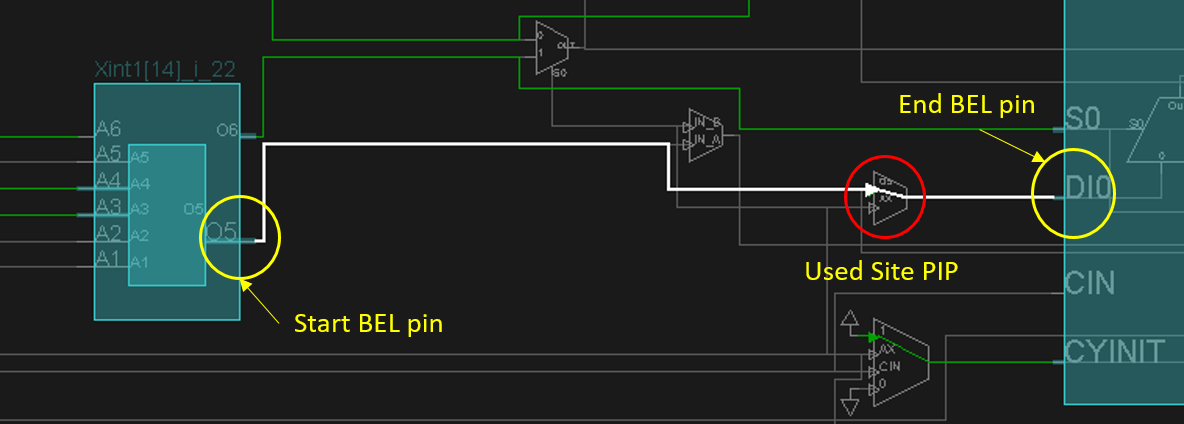
\includegraphics[width=\columnwidth]{sitePips.png}
  \caption{Site PIP Usage}
  \label{fig:sitePips2}
\end{figure}

\subsubsection{LUT Routethroughs} \label{sec:belRoutethroughs}
% TODO: explain here that no cell is placed on the bel?
Besides their use in implementing logic equations, LUT BELs can also be
configured as PIPs in a fully-routed FPGA design (known as a routethrough). A
LUT is marked as a routethrough when its configuration equation,
\texttt{CONFIG.EQN}, maps the value of a single input pin directly to the
output pin. For timing, the A6 pin is the most preferable option for
a routethrough since it is the fastest, but pins A1-A5 can also be
used in cases of routing congestion. Routethrough LUTs are not explicitly
represented in a design netlist since there is no cell placed on the
corresponding BEL, so they need to be included in the \textit{routing.rsc} of a
RSCP. Otherwise, designs could not be fully represented in external tools.
\autoref{fig:routethroughs2} shows two example routethrough LUTs in Vivado.

\begin{figure}[h]
  \centering
  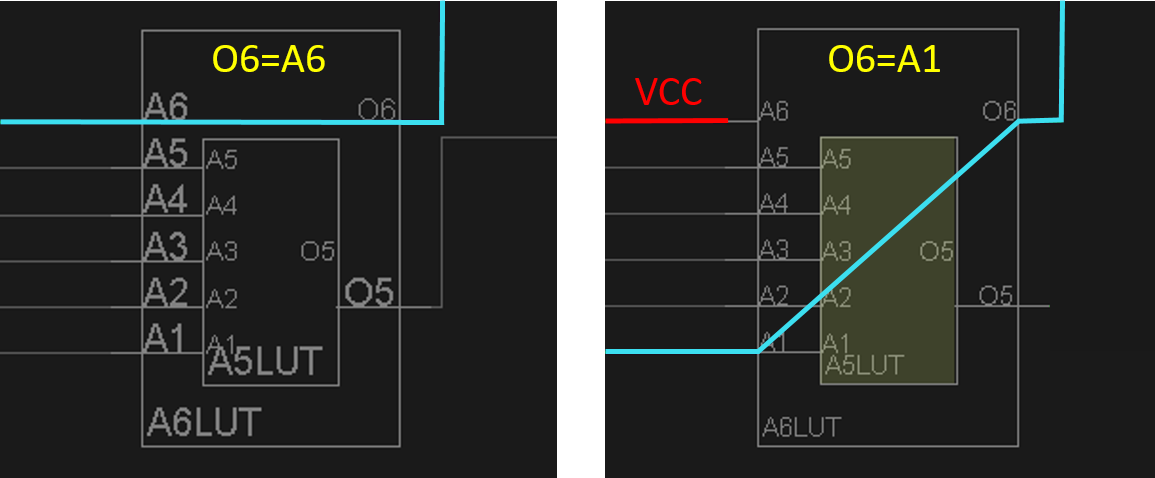
\includegraphics[width=5.5in]{routethroughs2.png}
  \caption{Two examples of LUTs configured as routethroughs in Vivado. The net
  highlighted in red represents VCC.}
  \label{fig:routethroughs2}
\end{figure}

For the LUT on the left, the input pin \texttt{A6} is mapped directly to the 
output pin \texttt{O6}. The corresponding configuration equation for this BEL is 
\texttt{CONFIG.EQN:O6=(A6)}. For the LUT on the right, the input pin \texttt{A1}
is mapped directly to the output pin \texttt{O6}. However, the structure of the
configuration equation for this LUT is slightly different. As 
\autoref{fig:routethroughs2} shows, VCC is routed to the \texttt{A6} input pin.
In this case, the configuration equation on the BEL is
\texttt{CONFIG.EQN:O6=(A6+{\textasciitilde}A6)*((A4))}. Using Vivado's TCL
interface, LUT routethroughs can be identified by matching their
\texttt{CONFIG.EQN} property against the Tcl regular expression

\begin{center}
\verb!(O[5,6])=(?:\(A6\+~A6\)\*)?\(+(A[1-6])\)+ ?!
.
\end{center}

On design export, LUTs that are identified as routethroughs are included
in the \textit{routing.rsc} file with the token \texttt{LUT\_RTS}. An example is
shown on line 6 of \autoref{lst:routingRsc}. Each routethrough is represented
in the form ``site/bel/input\_pin/output\_pin." It is important to note that not
all LUT BELs are tested for routethroughs. For an arbitrary LUT to be
used as a routethrough, it needs to satisfy three conditions. (1) Its parent
site needs to be used (i.e. there is at least one cell placed onto the site),
(2) no cell is currently placed on the corresponding bel, and (3) at least one
input bel pin is not currently being used.

\subsubsection{Permanent Latches}
A \textbf{permanent latch} in Vivado is a Flip Flop (FF) BEL which has been
configured as a latch with its ``set'' signal tied to VCC. This means that the
data pin of the latch always passes its value to the output pin of the latch,
and no state is retained. An example is shown in \autoref{fig:ffRoutethrough2}.
As the figure shows, permanent latches look very similar to LUT routethroughs
described in the previous section.

\begin{figure}[h]
  \centering
  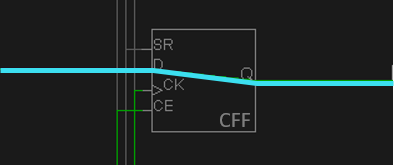
\includegraphics[width=.5\columnwidth]{ffRoutethrough.png}
  \caption{Flip-Flop BEL Configured as a Permanent Latch in Vivado}
  \label{fig:ffRoutethrough2}
\end{figure}

Because of this similarity, \textit{routing.rsc} files treat permanent latches
the same as LUT route-throughs. That is, each permanent latch is included
alongside the \texttt{LUT\_RTS} token as shown on line 6 of
\autoref{lst:routingRsc}. The string ``SLICE\_X40Y\-96/DFF/D/Q'' gives an
example of what a permanent latch looks like in the \textit{routing.rsc} file. Permanent
latches in Vivado can be identified based on two qualifications: (1) there is
no cell placed on the corresponding FF BEL, and (2) the property
\texttt{CONFIG.LATCH\_OR\_FF} of the BEL is set to \texttt{LATCH}.

\subsubsection{LUT Static Sources}
Similar to their use as routethroughs, LUT BELs can also be configured as GND or
VCC signal sources. Examples of both are shown in
\autoref{fig:lutStaticSources2}. The LUT on the left of the figure drives a VCC
signal and the LUT on the right drives GND. In both cases, the logical
netlist of a design does not represent the use of these LUTs in any way.
Therefore, the \textit{routing.rsc} file marks VCC and GND source LUTs with the
tokens \texttt{VCC\_SOURCES} and \texttt{GND\_SOURCES} respectively. This is
shown on line 4 and 5 of \autoref{lst:routingRsc}. External tools can use the
BELs marked \texttt{VCC\_SOURCES} and \texttt{GND\_SOURCES} to fully
recreate the routing of GND and VCC nets. Static source LUTs are identified
in Vivado by matching their \texttt{CONFIG.EQN} property against the Tcl regular
expression

\begin{center}
\verb!(O[5,6])=(?:\(A6\+~A6\)\*)?\(?[0,1]\)? ?!
.
\end{center}

\noindent LUTs that match the expression are formatted in
\textit{routing.rsc} with the form ``site/bel/source\_pin.'' It is important to
note that external CAD tools can also make use of this routing structure while
creating routing algorithms for Xilinx devices.

\begin{figure}[t]
  \centering
  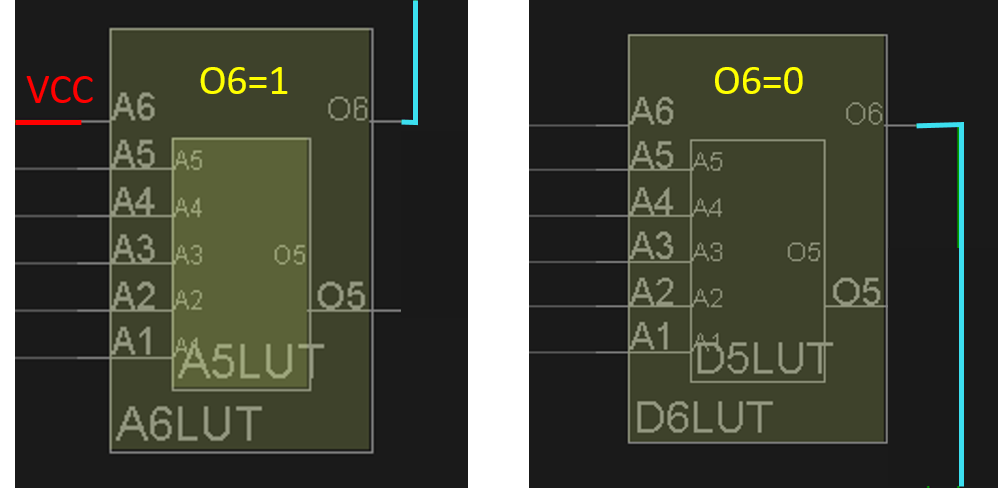
\includegraphics[width=.7\columnwidth]{lutStaticSources.png}
  \caption{Two LUTs Configured as Static Sources in Vivado}
  \label{fig:lutStaticSources2}
\end{figure}

\subsubsection{Intrasite Nets}

There are two types of nets in Vivado: \textbf{intrasite} nets and
\textbf{intersite} nets. Intrasite nets are those that are contained completely
within site boundaries. \autoref{fig:intrasite} shows an example intrasite net,
which connects to only BEL pins. The \textit{routing.rsc} file marks all
intrasite nets with the token \texttt{INTRASITE} as shown on line 8 of
\autoref{lst:routingRsc}. No additional information is given about
intrasite nets. External tools can reconstruct intrasite nets by using the
source BEL pin of the net in conjunction  with the used site pips of the
corresponding site. A list of intrasite nets can be obtained in Vivado with
the Tcl command \texttt{[get\_nets -filter \{ROUTE\_STATUS==INTRASITE\}]}.

\begin{figure}[b!]
  \centering
  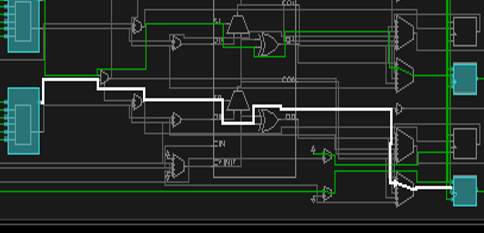
\includegraphics[width=.9\columnwidth, height=2in]{intrasite.png}
  \caption{Vivado Intrasite Net (highlighted in white)}
  \label{fig:intrasite}
\end{figure}

\subsubsection{Intersite Nets}

%Intersite nets have two different structures based on the current stage of
% design implementation.
A majority of nets in a FPGA design are \textbf{intersite} nets. Intersite nets
are those that use general routing fabric to connect cells across site
boundaries as shown in \autoref{fig:intersiteNet}.  After
a design has been placed in Vivado, each intersite net is partially routed.
That is, the intrasite portions of the net (the wires within sites) are routed
to site pins via site wires. To represent an intersite net at the placement
stage of implementation, the \textit{routing.rsc} file includes an
\texttt{INTERSITE} token, which lists all site pins a net is connected to. Line
9 of \autoref{lst:routingRsc} shows an example \texttt{INTERSITE}
specification. Site pins are important for recreating the routing structure of
nets in external tools because they can be used to (a) build the intrasite
portions of a net and (b) determine if a net is fully routed (nets that route
to all their site pins are fully routed by definition). In Vivado, the site pins
attached to a net can be determined with the Tcl command
\texttt{[get\_site\_pins -of \$net]}.

During the routing stage of implementation, all site pins of a net are connected
together through the general routing fabric of the FPGA. At this point the net
is considered fully routed. The physical structure of a fully routed net
can be expressed three different ways in Vivado:  (1) the ROUTE property on the
net, (2) the wires used in the net, or (3) the device PIPs used in the net. For
reasons discussed in Section~\ref{sec:tclChallenges}, device PIPs are the best option
for external tools. The \textit{routing.rsc} file uses the token \texttt{ROUTE}
for specifying the PIPs of a routed net. Line 10 of \autoref{lst:routingRsc}
shows an example \texttt{ROUTE} specification. The Tcl command
\texttt{[get\_pips -of \$net]} can be used to get a list of all PIPs being used
in a Vivado net. The RapidSmith2 import code contains an algorithm to convert
the pip list to a tree structure.

\begin{figure}[t!]
  \centering
  \includegraphics[width=.4\columnwidth]{intersiteNet.png}
  \caption{Vivado Intersite Net (highlighted in white)}
  \label{fig:intersiteNet}
\end{figure}

\subsubsection{VCC and GND Nets}

In general, a design can have more than one VCC net in the logical netlist. Each
of these nets should have their own unique physical information once the
design is routed (based on which wires they use), but this is not the case with
Vivado. Instead, Vivado reports that they each use the same set of wires which
correspond to a combination of \textit{all} VCC nets. The same applies to GND
nets. There are two possible solutions to resolve this discrepancy. The first is
to merge all logical VCC (or GND) nets in the netlist into a single net, matching
the merged physical routing. The second is to partition the physical
information so that each logical net has unique physical properties. 

For simplicity, RSCPs choose to implement the first option. Lines 12-15 of
\autoref{lst:routingRsc} show how VCC and GND nets are represented in a
\textit{routing.rsc} file. The \texttt{VCC} and \texttt{GND} tokens serve the
same purpose as \texttt{ROUTE}, they contain the used PIPs for all VCC and GND
nets. The \texttt{START\_WIRES} token gives a list of all wires connected to
VCC and GND sources. Starting at the specified start wires, VCC and GND nets
can be reconstructed in external tools. The Tcl command \texttt{[get\_nets
-filter \{TYPE==POWER\}]} is used to find all VCC nets in a design, and
\texttt{[get\_nets -filter \{TYPE==GROUND\}]} is used to find all GND nets
in a design. The start wires for VCC and GND nets are found by parsing their
corresponding \texttt{ROUTE} property strings.

%%%%%%%%%%%%%%%%%%%%%%%%%%%%%%%%%%%%%%%%%%%%
%				TCPs
%%%%%%%%%%%%%%%%%%%%%%%%%%%%%%%%%%%%%%%%%%%%
\subsection{Design Import (TCP Format)} \label{sec:vdiExport}

RSCPs are only used to represent exported Vivado designs and cannot be directly
imported back into Vivado. They must first be converted to \textbf{Tincr
Checkpoints} (TCP) in an external tool or framework. TCPs are a fileset proposed
in the original \texttt{Tincr} distribution, and serve as an alternate
representation of Vivado designs which can be imported into Vivado through the
VDI interface. Each TCP contains the following four files:

\begin{multicols}{2}
	\begin{itemize}
	  \item netlist.edf
	  \item constraints.xdc
	  \item placement.xdc
	  \item routing.xdc
	\end{itemize}
\end{multicols}

\noindent As can be seen, TCPs are largely based on Vivado XDC files, which
allow a subset of Tcl commands to set constraints on a variety
of Vivado objects. For example, cells can be placed and nets can be routed with
XDC constraints. The XDC format is desirable for two reasons in particular: (1)
a single Vivado Tcl command \texttt{[read\_xdc]} can parse and apply XDC
constraint files and (2) \texttt{[read\_xdc]} is much faster than regular Tcl
scripts executing the same commands.

Each file in a TCP represents a specific aspect of a Vivado FPGA design, and is
described in the following subsections as a review for the reader. The
\textit{netlist.edf} and \textit{contraints.xdc} file will not be reviewed
because they are identical to their RSCP counterparts presented in
Section~\ref{sec:vdiImport}. The \texttt{Tincr} function used to parse TCPs,
\texttt{[tincr::read\_tcp]}, has been updated in a variety of ways to support
fully importing Vivado designs. These modifications, and the limitations of
XDC, are described more in Section~\ref{sec:tclChallenges}

\subsubsection{Placement.xdc}
\autoref{lst:placementXdc} shows an example \textit{placement.xdc} file within a
TCP. Lines 1-3 of the listing show how a cell is placed in Vivado using XDC
commands. As can be seen, the first command sets the \texttt{BEL} property on
the cell to the corresponding \texttt{SITE\_TYPE.BEL\_NAME}. The second command
sets the \texttt{LOC} property on the cell, which specifies the actual site
location. The ordering of these commands relative to one another is crucial,
because if the \texttt{LOC} property is set before the \texttt{BEL} property an
error will be thrown in Vivado. For cells of group \texttt{LUT}, \texttt{INV},
or \texttt{BUF} the cell pin to BEL pin mappings must be set manually by the user. 
This can be done by setting the \texttt{LOCK\_PINS} property on the cell as
shown on line 3, and is most often used for LUT cells. Line 4 of
\autoref{lst:placementXdc} shows how a top-level port is mapped  to a FPGA
package pin.

\begin{lstlisting}[xleftmargin=1.5em, framexleftmargin=1.5em, keywordstyle=,
stringstyle=, caption= Sample placement.xdc, label=lst:placementXdc]
	set_property BEL SLICEM.H6LUT [get_cells {u3/angle.Ao[16]_i_3}]
	set_property LOC SLICE_X50Y30 [get_cells {u3/angle.Ao[16]_i_3}]
	set_property LOCK_PINS { I0:A3 I1:A1 } [get_cells {u3/angle.Ao[16]_i_3}]
	...
	set_property PACKAGE_PIN AD10 [get_ports {Rout[16]}]
	...	
\end{lstlisting}

\subsubsection{Routing.xdc} \label{sec:routingXdc}
During placement, the intrasite routing structure of each site is automatically
configured in Vivado based on what cells are placed onto the corresponding site.
Therefore, the only necessary information in the \textit{routing.xdc} file is
the intersite routing specification for each net. Specifically, the physical
structure of a net is specified in Vivado by setting its \texttt{ROUTE} string
property (also called a directed routing string) as shown in \autoref{lst:routingXdc}.
A directed routing string represents the tree structure of a physical
route by using nested brackets (``\{'') to represent branching. As an example,
take the hypothetical route shown in \autoref{fig:routeString}. One valid
\texttt{ROUTE} string associated with this route is \texttt{\{ A B \{ D E \} C
\}}. Another possible \texttt{ROUTE} string is \texttt{\{ A B \{ C \} D E \}},
they both represent the route shown in the figure. \texttt{ROUTE} strings can be
formatted to either include the tile of each wire (line 2 of
\autoref{lst:routingXdc}), or use only relative wire names (line 3 of
\autoref{lst:routingXdc}). The advantage of including tile names is to remove
any possible ambiguity for a route. The advantage of using relative wire names
is that they result in smaller \textit{routing.xdc} files. It is considered
best practice, however, to format \texttt{ROUTE} strings using tile names
to ensure the correctness of the route when it is imported into Vivado. 

\begin{lstlisting}[xleftmargin=1.5em, framexleftmargin=1.5em,keywordstyle=,
stringstyle=, caption= Sample routing.xdc, label=lst:routingXdc]
	...
	set_property ROUTE { CLEL_R_X36Y8/CLE_L_SITE_0_COUT ... }  [get_nets {Zo}]
	set_property ROUTE { CLE_L_SITE_0_COUT ... }  [get_nets {Zo}]
	...
\end{lstlisting}

\begin{figure}[t!]
  \centering
  \includegraphics[width=.8\columnwidth]{routeString.eps}
  \caption{Sample Route (A, B, C, D, and E represent device wires)}
  \label{fig:routeString}
\end{figure}

%%%%%%%%%%%%%%%%%%%%%%%%%%%%%%%%%%%%%%%%%%%%
%		Tcl Interface Challenges
%%%%%%%%%%%%%%%%%%%%%%%%%%%%%%%%%%%%%%%%%%%%
\subsection{Vivado Tcl Interface Challenges} \label{sec:tclChallenges}

Vivado's Tcl interface supplies the necessary functionality to generate and
parse external design representations. VDI uses the interface to define the
formats for RSCPs and TCPs as described in the previous sections. There are,
however, a variety of challenges associated with using Tcl commands to generate
RSCPs and parse TCPs. Broadly, these challenges can be grouped into four
distinct categories.

\begin{enumerate}
  \item Vivado design import rules: External designs need to be imported
  into Vivado in a very specific way, or else import can fail. 
  \item Logical to physical mismatches: When a netlist is implemented on a
  device, most physical components match to a corresponding logical component
  (i.e. a BEL maps to a cell). But, there are some aspects of an
  implemented design that aren't represented in the logical netlist.
  \item Tcl objects that are incomplete, ambiguous, or return incorrect
  results when queried.
  \item Parts of a device or design that cannot be configured with Tcl commands
\end{enumerate}

\noindent The following subsections document each issue associated with
generating RSCPs or parsing TCPs, with their appropriate workaround. In some
cases, it is up to external tools to provide a solution. As previously
mentioned, each of these issues is specific to Vivado 2016.2, and may be fixed
in future tool versions.

%and help give a better understanding of why
%two different external design representations are necessary. 

\subsubsection{Ambiguous ROUTE Strings} \label{sec:routeStrings}

As described in Section~\ref{sec:routingXdc}, the \texttt{ROUTE} property
on a net contains its physical routing structure. By default, Vivado uses
relative wire names (no tile information) when building these \texttt{ROUTE}
strings. This is problematic for external tools because it can lead to wire
ambiguities. Specifically, it is possible for a given wire in a Xilinx FPGA
to connect to more than one wire of the same name. The 
\texttt{BRAM\_L\_X6Y170/BRAM\_CASCOUT\_ADDRBWRADDRU6} wire in the Artix7 part
\texttt{xc7a100tcsg324-3} is an example. This wire connects to two different
wires named \texttt{BRAM\_ADDRBWRADDRU6} through PIP connections.
The first wire is located in tile \texttt{BRAM\_L\_X6Y165} and the second wire
is located in tile \texttt{BRAM\_L\_X6Y175}. \autoref{lst:ambigRoute} shows how
Vivado distinguishes these two connections within \texttt{ROUTE} strings.

\begin{lstlisting}[xleftmargin=1.5em, framexleftmargin=1.5em, keywordstyle=,
stringstyle=, caption= Ambiguous ROUTE string example, label=lst:ambigRoute, escapeinside=||]
	// Tile  BRAM_L_X6Y165
	{ ...  BRAM_CASCOUT_ADDRBWRADDRU6 BRAM_ADDRBWRADDRU6  ... }
	// Tile BRAM_L_X6Y175 
	{ ...  BRAM_CASCOUT_ADDRBWRADDRU6 |\textbf{<1>}|BRAM_ADDRBWRADDRU6  ... }
\end{lstlisting}

\noindent As can be seen, the token ``\textless1\textgreater" is used to
differentiate the two wires. Vivado most likely has an internal data
structure that uses the token to choose the correct sink wire.  External
tools, however, don't have access to this data structure, meaning the only
option is to guess which wire is actually taken (clearly not an acceptable
solution). Ambiguous \texttt{ROUTE} strings are the primary reason why RSCPs use
PIPs to represent routing, and two different external formats are required.
 
\subsubsection{Alternate Site Pins}

As discussed in Section~\ref{sec:alternateSites}, the Vivado Tcl command
\texttt{[get\_site\_pins -of \$site]} does not return the correct result for
alternate sites on Series7 devices\footnote{UltraScale devices always return
the correct result}. An example of this behavior is shown in
\autoref{fig:alternateSitePins}. The site pin names clearly change in the GUI
after the site is changed to be of type \texttt{RAMB18E1}, but the Tcl
interface is not updated accordingly. RSCPs depend on exporting a correct set
of site pins for each net, but the reported site pins will be incorrect for
alternate sites if the above command is used.

\begin{figure}[h!]
  \centering
  \includegraphics[width=\columnwidth]{alternateSitePins.png}
  \caption{An example of [get\_site\_pins] returning incorrect results in
  Vivado}
  \label{fig:alternateSitePins}
\end{figure}

VDI fixes this issue with an assumption about single-BEL sites in Series7
devices. As can be seen in \autoref{fig:alternateSitePins}, each BEL pin within
a single-BEL site connects to an identically named site pin. Using this
assumption and a customized site pin getter, the VDI command
\texttt{[tincr::write\_rscp]} reports the correct site pins for each net
connected to an alternate site. Of course, this is only valid if all alternate
types with changing site pins have a single BEL. Through experimentation
with several different designs, this appears to be true. As more tests are run
on Series7 devices and designs, the conclusion will be further tested for
validity.

\subsubsection{VCC/GND BEL Pins} \label{sec:vccGndBelPins}
% TODO: see if we can determine this in Vivado by looking at a nets BEL pins.
Most nets in a Vivado design connect to a set of cell pins, and are routed to
the corresponding BEL pins of those cell pins. VCC and GND nets,
however, can route directly to BEL pins that don't have a connecting cell pin.
An example is shown in \autoref{fig:pseudoCellPin2}. As the figure shows, VCC is
routed to the \texttt{A6} pin of the \texttt{D6LUT}, but there is no cell pin
mapped to \texttt{A6} (the input pins of the cell placed at the LUT have
been mapped to \texttt{A1} and \texttt{A4}). The fact that VCC connects to the
\texttt{A6} pin of this LUT is not represented in the logical netlist, and is purely an
implementation detail of the design. Lacking this information is particularly
challenging when developing routing algorithms in external tools. How will the
algorithm know to route to VCC/GND BEL pins when they are not explicitly
represented in the netlist? Unfortunately, these BEL pins cannot currently be
determined with Vivado Tcl commands, and so are not included in RSCPs. It is up
to external tools to understand the placement configurations that require VCC
and GND to be routed to individual BEL pins.

\begin{figure}[t]
  \centering
  \includegraphics[width=.6\columnwidth]{pseudoCellPin.png}
  \caption{An example of VCC routing to an unused BEL pin (A6)}
  \label{fig:pseudoCellPin2}
\end{figure}

\subsubsection{SLICE Placement Order} \label{sec:slicePlacementOrder}

\begin{figure}[b!]
  \centering
  \includegraphics[width=\columnwidth]{contention.png}
  \caption{Routing Contention Example}
  \label{fig:contention}
\end{figure}

When a cell is placed in Vivado using Tcl API calls, Vivado
automatically configures the routing resources inside of the
corresponding site based on the cell's connections. Because
of this behavior it is possible to have a valid cell placement,
but to place the cells in an order that causes an illegal routing
configuration (i.e. a routing mux is optionally being used by
a net, but is required by a different net of a cell that has just
been placed). This primarily affects sites of type SLICEL
and SLICEM, due to their more complex internal routing. 

\autoref{fig:contention} shows a simplified example of why routing contention
can happen within SLICE sites. In this hypothetical scenario, the netlist in
the left of the figure is  placed onto the site in the right of the 
figure. Assume the cells of the netlist are placed in the following
order: (1) \texttt{A} $\,\to\,$ LUT1, (2) \texttt{C} $\,\to\,$ FF1, and (3)
\texttt{B} $\,\to\,$ FF2. Cell \texttt{A} will first be placed onto the LUT1 BEL
which will use the mux to leave the site because its downhill cell (\texttt{B})
has not yet been placed. When cell \texttt{C} is placed on the FF1 BEL, an error
will be thrown because the net connected to \texttt{C} needs to be routed
outside of the site, but the routing mux is already in use and there is no
other way to leave the site. At this point placement has failed. If instead the
placement order is (1) \texttt{B} $\,\to\,$ FF2, (2) \texttt{A} $\,\to\,$ LUT1,
and (3) \texttt{C} $\,\to\,$ FF1, no routing contention will happen because the
site mux will be available once cell \texttt{C} is placed.

\begin{figure}[t!]
  \centering
  \includegraphics[width=.7\columnwidth]{slicePlacementOrder.png}
  \caption{Required placement order for Series7 SLICE sites. The figure shows a
  simplified representation of a SLICEL site.}
  \label{fig:slicePlacementOrder}
\end{figure}


For Series7 devices, experimentation has shown that the proper placement order
for groups of cells mapped to SLICE sites is as shown in
\autoref{fig:slicePlacementOrder}. The D6LUT needs to be placed first for
distributed memory cells. If the required placement order is not followed when
recreating a design, internal routing conflicts will occur that Vivado will be
unable to resolve. It is the responsibility of external tools to sort the cells
of a design in the proper order shown in \autoref{fig:slicePlacementOrder} when
creating the \textit{placement.rsc} file of a TCP.

It is important to note that the SLICE architecture of UltraScale
devices is significantly different than the Series7. Specifically, SLICE sites
in UltraScale have 8 LUTs (H-A), 16 FFs, and a CARRY8 instead of a CARRY4. In
initial testing, it appears that the placement order for UltraScale designs is
less strict. The only requirement is that the H6LUT (top-most LUT in the SLICE)
be placed first for distributed memory.

\subsubsection{Macro Placement} \label{sec:macroPlacement}

As described in Section~\ref{sec:macros} fully-flattened Vivado netlists may
include macro primitives. Section~\ref{sec:vdiImport} describes how macros
are exported from Vivado in RSCP files. Importing macro primitives
back into Vivado using TCP files, however, is a little more complicated. This
is because internal cells to a macro cannot be placed with XDC Tcl commands
(setting the property of an internal cell is an unauthorized operation in
Vivado). Therefore, external tools have two options when generating a TCP with
macros:

\begin{enumerate}
  \item Before creating the TCP, completely flatten the design netlist so that
  all macros are completely removed from the design.
  
  \item Support relatively placed macros (RPM), and output the placement
  information for just the RPM (not the internal cells) to the TCP. RPMs are
  macro cells that are assigned an anchor BEL placement location, and internal
  cells to the macro are placed \textit{relative} to the anchor.
\end{enumerate}

\noindent In general, the easier of the two solutions is to flatten the
design netlist completely, but either solution is valid with VDI. 

\subsubsection{LUT Routethroughs} \label{sec:routethroughReplace}

As described in Section~\ref{sec:routingRsc}, the \texttt{CONFIG.EQN} property on a
LUT BEL can be used to identity it as routethrough. On design export, all LUTs
in a design whose configuration equation matches that of a routethrough are
marked in the generated RSCP. It would stand to reason that when importing a
design back into Vivado, routethroughs could be recreated by setting the
corresponding \texttt{CONFIG.EQN} of the BEL. \texttt{CONFIG.EQN}, however, is
a \textbf{read-only} property, meaning the value can be queried but not
modified. Explicitly configuring a BEL's properties using the Tcl command
\texttt{[set\_property]} will throw an error in Vivado. These properties can
only be modified internally during the placement or routing stage of
implementation. Due to these limitations, it is currently not possible
to configure a BEL LUT as a routethrough in Vivado.

Therefore, it is the responsibility of external tools to replace all LUT
routethroughs in a design with a Xilinx \texttt{LUT1} cell before generating a
TCP. The general method for this is shown in \autoref{fig:routethroughReplace}.

\begin{figure}[h]
  \centering
  \includegraphics[width=\columnwidth]{routethroughReplace.png}
  \caption{Visualization for how to replace a LUT routethrough with a LUT1 Xilinx cell.}
  \label{fig:routethroughReplace}
\end{figure}

\noindent First, disconnect the routethrough net from all
downhill sink cell pins. Next, create a new \texttt{LUT1} Xilinx
library cell with a unique name and set the cell's \texttt{INIT} property to
``2'h2'' (this configures the cell to be a passthrough LUT). Place the cell
onto the BEL that was formerly being used as a routethrough, and map the
\texttt{I0} input pin of the cell to the corresponding routethrough BEL pin
(\texttt{A1} in the case of the example). Rewire the netlist and connect
the original routethrough net to pin \texttt{I0} of the new cell. The final
step is to create a new net with a unique name, and connect it to the
output pin of the new cell and the downhill logic disconnected earlier. Once
this is complete, the netlist now explicitly represents the routethrough, and
valid TCPs can be generated.

\subsubsection {Routing Differential Pairs}
Xilinx devices support differential input signals for design input. An example
differential pairing is shown in \autoref{fig:diffInput}. The net highlighted in
white connects the two differential signals together for Xilinx to resolve to a
single value. As can be seen, the physical route of the net is very simple, with
only a single PIP connection. As a TCP is being imported, however, Vivado is
unable to correctly process the \texttt{ROUTE} strings for these nets.
Specifically, when the \texttt{ROUTE} string for a differential net is
specified, the following error message is given: ``\texttt{ERROR: [Designutils
20-949] No driver found on net netname}''. 

The function \texttt{[tincr::read\_tcp]} provides a workaround by first routing
all other nets in the design. Once all other nets have been routed, the Tcl code
shown in \autoref{lst:diffNet} is run. The differential nets are identified
using the Tcl command on line 1, and each net is individually routed by Vivado's
router. Since there is only one possible route between the source and the sink
pin, the differential nets will be routed correctly. The downfall to this
approach is that it can take up to 1 minute to finish routing all differential
nets. It is important to note that this is only an issue for Series7 devices,
and is not needed for UltraScale.

\begin{lstlisting}[xleftmargin=1.5em, framexleftmargin=1.5em, keywordstyle=,
stringstyle=, caption= Tcl script to route differential nets in Vivado, label=lst:diffNet]
set diff [get_nets -of [get_ports] -filter {ROUTE_STATUS != INTRASITE} -quiet]

if {[llength $diff] > 0 } {
	route_design -quiet -nets $diff
}
\end{lstlisting}

\begin{figure}[t!]
  \centering
  \includegraphics[width=.6\columnwidth]{diffInput.png}
  \caption{Differential Pair Net}
  \label{fig:diffInput}
\end{figure}

\subsection{Why Two Design Checkpoint Formats?} \label{sec:twoFormats}
So far this chapter has described in great detail RSCPs, TCPs, and the
associated Vivado Tcl challenges with both. There is, however, one more
question to consider: ``Why can't a single design format be used for external
tools \textit{and} Vivado''? Here are four reasons why both RSCPs and TCPs are
required with VDI:

\begin{enumerate}
  \item Some Vivado design representations cannot be used with
  external tools. This is best shown with Vivado \texttt{ROUTE} strings, which
  are used to represent the physical route of a net. Due to the ambiguities of
  \texttt{ROUTE} strings as described in Section~\ref{sec:routeStrings}, they are
  not suitable for design export (PIPs must be used instead). However,
  \texttt{ROUTE} strings are required when importing a design back into Vivado
  (Section~\ref{sec:routingXdc}). This indicates that a different format is needed
  for exporting and importing the physical structure of a net.
     
  \item When an external design is imported into Vivado, some physical
  implementation details of the design are automatically configured. 
  For example, site PIPs, static source LUTs, and intrasite nets are all
  configured during placement import based on how the cells of a design are
  placed. These design aspects do not need to be explicitly represented in a
  TCP. External tools don't have the luxury of automatic configuration, and so
  these details do need to be explicitly represented in a RSCP. Otherwise, a
  design could only be partially represented.
    
  \item RSCPs and TCPs are designed for different purposes. TCPs are
  designed to import a design into Vivado as \textbf{quickly as possible}. The
  XDC format allows for this due to the dedicated Tcl command
  \texttt{[read\_xdc]}. RSCPs are designed to be \textbf{easily parse-able}, and
  use a simple token-based scheme with whitespace separated values.
  
  \item Vivado offers a native checkpoint format (DCP) that can be used to save
  and restore the progress of an implemented design. Due to this available
  checkpoint format, there is no reason to support importing RSCPs directly back
  into Vivado. Users that want this capability can use DCPs, allowing RSCP
  checkpoints to be more customized.
  
\end{enumerate}

\end{document}
%%%%%%%%%%%%%%%%%%%%%%%%%%%%%%%%%%%%%%%%%%
%	Document End
%%%%%%%%%%%%%%%%%%%%%%%%%%%%%%%%%%%%%%%%%%
